\documentclass[10pt,letterpaper]{article}\usepackage[]{graphicx}\usepackage[]{color}
%% maxwidth is the original width if it is less than linewidth
%% otherwise use linewidth (to make sure the graphics do not exceed the margin)
\makeatletter
\def\maxwidth{ %
  \ifdim\Gin@nat@width>\linewidth
    \linewidth
  \else
    \Gin@nat@width
  \fi
}
\makeatother

\definecolor{fgcolor}{rgb}{0.345, 0.345, 0.345}
\newcommand{\hlnum}[1]{\textcolor[rgb]{0.686,0.059,0.569}{#1}}%
\newcommand{\hlstr}[1]{\textcolor[rgb]{0.192,0.494,0.8}{#1}}%
\newcommand{\hlcom}[1]{\textcolor[rgb]{0.678,0.584,0.686}{\textit{#1}}}%
\newcommand{\hlopt}[1]{\textcolor[rgb]{0,0,0}{#1}}%
\newcommand{\hlstd}[1]{\textcolor[rgb]{0.345,0.345,0.345}{#1}}%
\newcommand{\hlkwa}[1]{\textcolor[rgb]{0.161,0.373,0.58}{\textbf{#1}}}%
\newcommand{\hlkwb}[1]{\textcolor[rgb]{0.69,0.353,0.396}{#1}}%
\newcommand{\hlkwc}[1]{\textcolor[rgb]{0.333,0.667,0.333}{#1}}%
\newcommand{\hlkwd}[1]{\textcolor[rgb]{0.737,0.353,0.396}{\textbf{#1}}}%
\let\hlipl\hlkwb

\usepackage{framed}
\makeatletter
\newenvironment{kframe}{%
 \def\at@end@of@kframe{}%
 \ifinner\ifhmode%
  \def\at@end@of@kframe{\end{minipage}}%
  \begin{minipage}{\columnwidth}%
 \fi\fi%
 \def\FrameCommand##1{\hskip\@totalleftmargin \hskip-\fboxsep
 \colorbox{shadecolor}{##1}\hskip-\fboxsep
     % There is no \\@totalrightmargin, so:
     \hskip-\linewidth \hskip-\@totalleftmargin \hskip\columnwidth}%
 \MakeFramed {\advance\hsize-\width
   \@totalleftmargin\z@ \linewidth\hsize
   \@setminipage}}%
 {\par\unskip\endMakeFramed%
 \at@end@of@kframe}
\makeatother

\definecolor{shadecolor}{rgb}{.97, .97, .97}
\definecolor{messagecolor}{rgb}{0, 0, 0}
\definecolor{warningcolor}{rgb}{1, 0, 1}
\definecolor{errorcolor}{rgb}{1, 0, 0}
\newenvironment{knitrout}{}{} % an empty environment to be redefined in TeX

\usepackage{alltt}
\usepackage[top=0.85in,left=1.75in,footskip=0.75in]{geometry}

% amsmath and amssymb packages, useful for mathematical formulas and symbols
\usepackage{amsmath,amssymb}

% Use adjustwidth environment to exceed column width (see example table in text)
\usepackage{changepage}

% Use Unicode characters when possible
\usepackage[utf8x]{inputenc}

% textcomp package and marvosym package for additional characters
\usepackage{textcomp,marvosym}

% cite package, to clean up citations in the main text. Do not remove.
\usepackage{cite}

% Use nameref to cite supporting information files (see Supporting Information section for more info)
\usepackage{nameref,hyperref}

% line numbers
\usepackage[right]{lineno}

% ligatures disabled
\usepackage{microtype}
\DisableLigatures[f]{encoding = *, family = * }

% color can be used to apply background shading to table cells only
\usepackage[table]{xcolor}

% array package and thick rules for tables
\usepackage{array}

% adjust width of tikz tables or figures
\usepackage{adjustbox}

% bold math symbols package
\usepackage{bm}

% nice figures and captions
\usepackage{graphicx}

% diagrams or complicated equations
\usepackage{tikz}

% vertical and horizontal dashed lines
\usepackage{arydshln}

%\usepackage{floatflt}
%\usepackage{nonfloat}
\usepackage{float}
\usepackage{wrapfig}

%\renewcommand{\arraystretch}{1.2}
%\setlength{\tabcolsep}{12pt}

% create "+" rule type for thick vertical lines
\newcolumntype{+}{!{\vrule width 2pt}}

% create \thickcline for thick horizontal lines of variable length
\newlength\savedwidth
\newcommand\thickcline[1]{%
  \noalign{\global\savedwidth\arrayrulewidth\global\arrayrulewidth 2pt}%
  \cline{#1}%
  \noalign{\vskip\arrayrulewidth}%
  \noalign{\global\arrayrulewidth\savedwidth}%
}

% \thickhline command for thick horizontal lines that span the table
\newcommand\thickhline{\noalign{\global\savedwidth\arrayrulewidth\global\arrayrulewidth 2pt}%
\hline
\noalign{\global\arrayrulewidth\savedwidth}}


% Remove comment for double spacing
%\usepackage{setspace} 
%\doublespacing

% Text layout
% \raggedright
\setlength{\parindent}{0.5cm}
\textwidth 5.25in 
\textheight 8.75in

% Bold the 'Figure #' in the caption and separate it from the title/caption with a period
% Captions will be left justified
\usepackage[aboveskip=1pt,labelfont=bf,labelsep=period,justification=raggedright,singlelinecheck=off]{caption}
\DeclareCaptionLabelFormat{Sformat}{S#2 #1}
\captionsetup[figure]{labelformat=Sformat} 
\renewcommand{\figurename}{Fig}
%\renewcommand{\figurename}{S\arabic{figure} Fig}
%\renewcommand{\thefigure}{S\arabic{figure} Fig}

% Use the PLoS provided BiBTeX style
%\bibliographystyle{plos2015}


% Remove brackets from numbering in List of References
\makeatletter
\renewcommand{\@biblabel}[1]{\quad#1.}
\makeatother

% define theorem and definition environments commands
\newtheorem{theorem}{Theorem}[section]
\newtheorem{definition}{Definition}[section]

% Header and Footer with logo
\usepackage{lastpage,fancyhdr,graphicx}
\usepackage{epstopdf}
%\pagestyle{myheadings}
\pagestyle{fancy}
\fancyhf{}
%\setlength{\headheight}{27.023pt}
%\lhead{\includegraphics[width=2.0in]{PLOS-submission.eps}}
\rfoot{\thepage/\pageref{LastPage}}
\renewcommand{\headrulewidth}{0pt}
\renewcommand{\footrule}{\hrule height 2pt \vspace{2mm}}
\fancyheadoffset[L]{2.25in}
% \fancyfootoffset[L]{1.25in}
\lfoot{\today}


\restylefloat{figure}


%% Include all macros below

\newcommand{\lorem}{{\bf LOREM}}
\newcommand{\ipsum}{{\bf IPSUM}}

\def\lf{\left\lfloor}   
\def\rf{\right\rfloor}

\def\ri{R_i}
\def\rj{R_j}
\def\kmi{k_{M_i}}
\def\khi{k_{H_i}}
\def\hji{H_{j_i}}
\def\ma{\overline{M}_a}
\def\ha{\overline{H}_a}
\def\mnu{M_\nu}
\def\hnu{H_\nu}
\def\myd{\text{diff}}
\def\ka{\bar{k}_\alpha}
\def\mji{M_{j_i}}

%% END MACROS SECTION
\IfFileExists{upquote.sty}{\usepackage{upquote}}{}
\begin{document}
\vspace*{0.2in}

% Title must be 250 characters or less.
% \begin{flushleft}
{\Large	
	\textbf\newline{Theoretical properties of distance distributions and novel metrics for nearest-neighbor feature selection: \\ Supplementary figures} % Please use "sentence case" for title and headings (capitalize only the first word in a title (or heading), the first word in a subtitle (or subheading), and any proper nouns).	
}

\begin{figure}[H]
	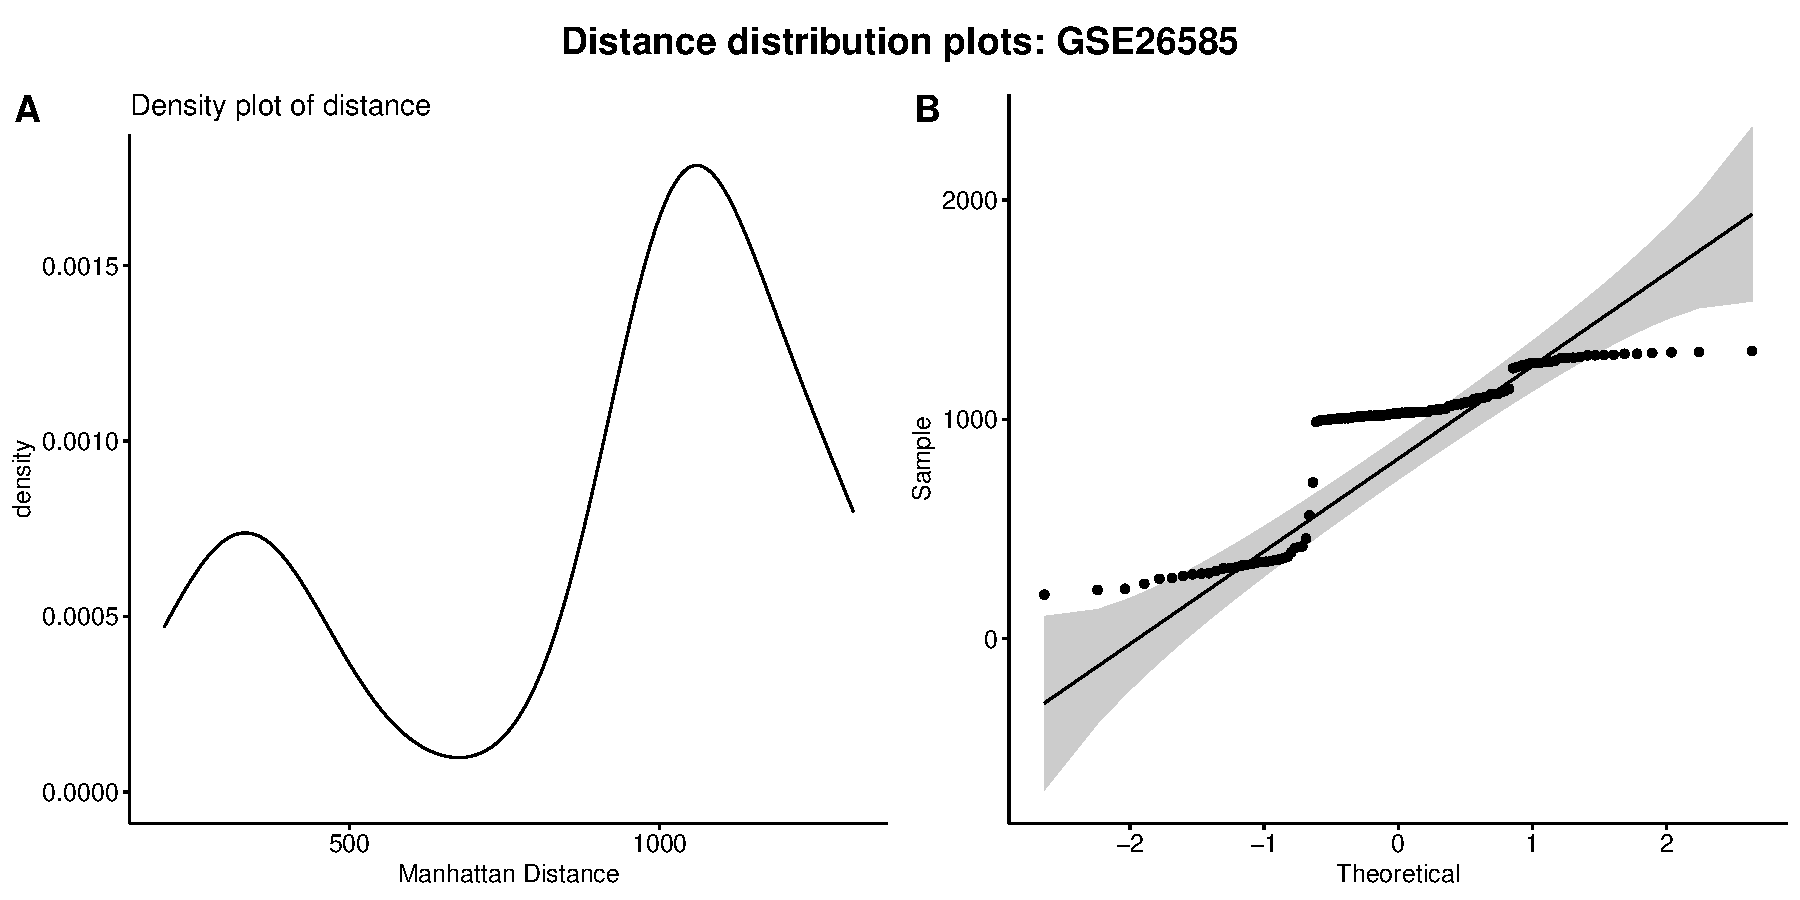
\includegraphics[width=\textwidth]{manhattan-distance_hist_GSE26585.pdf}
	\caption{Density and quantile-quantile plots for distances between samples in GSE26585. \textbf{A} Estimated density curve for distances. \textbf{B} Quantile-quantile plot between theoretical (standard normal) quantiles and sample distance quantiles.}
\end{figure}

\begin{figure}[H]
	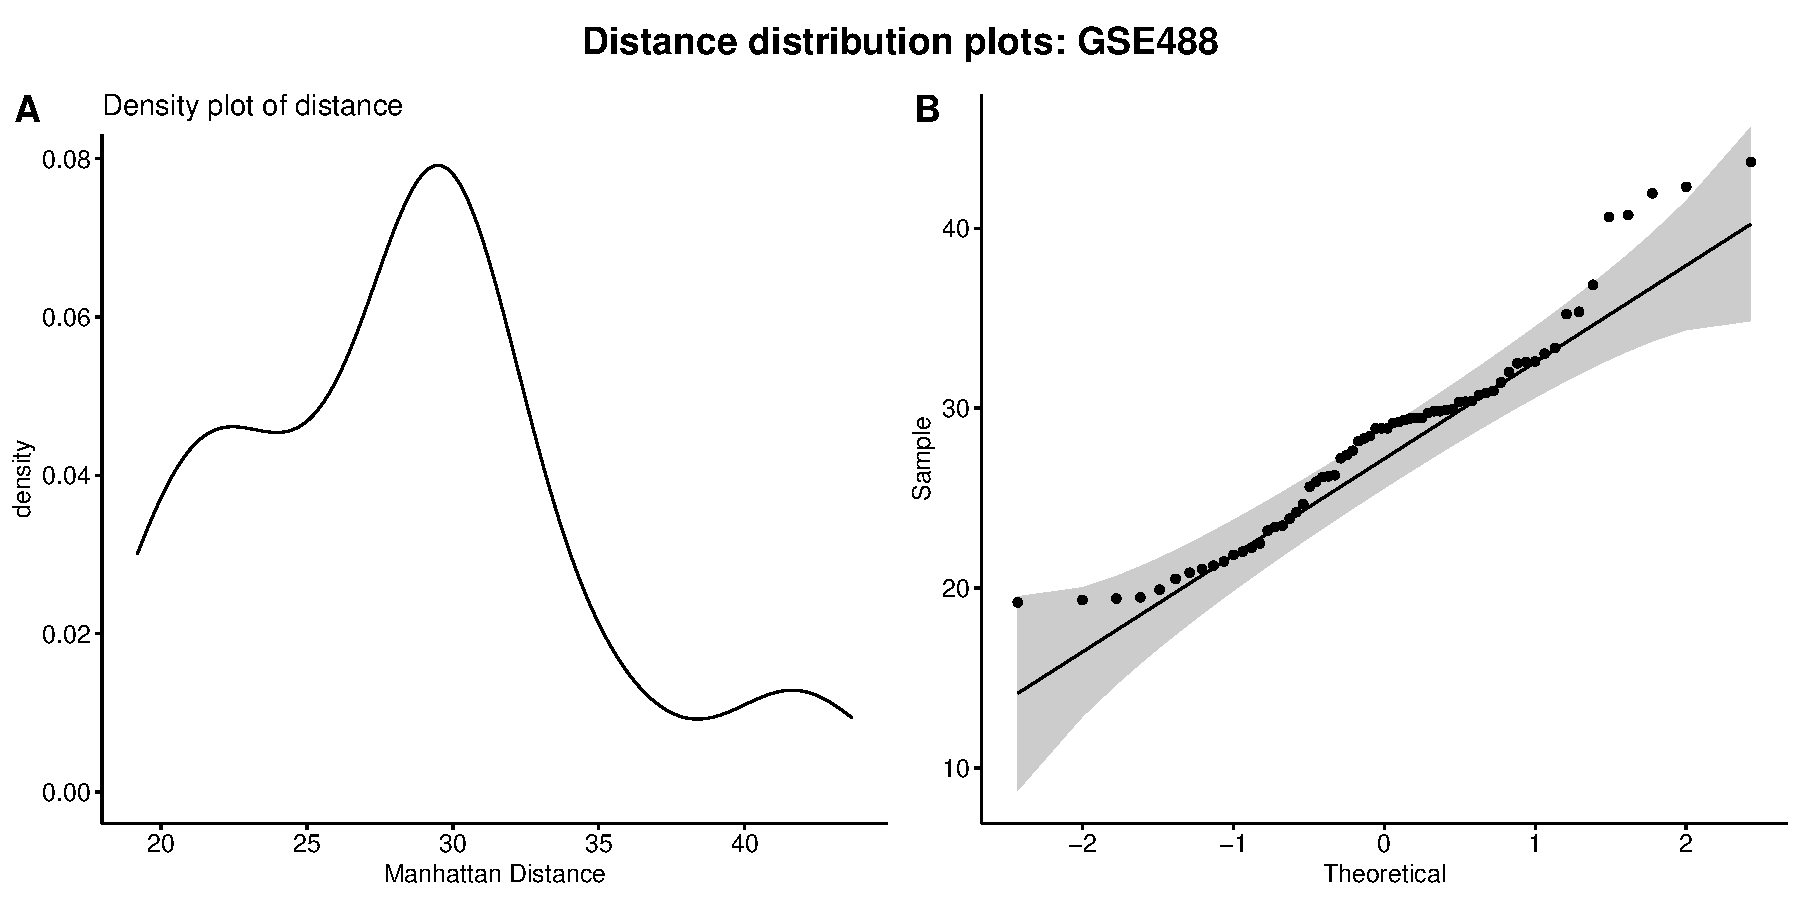
\includegraphics[width=\textwidth]{manhattan-distance_hist_GSE488.pdf}
	\caption{Density and quantile-quantile plots for distances between samples in GSE488. \textbf{A} Estimated density curve for distances. \textbf{B} Quantile-quantile plot between theoretical (standard normal) quantiles and sample distance quantiles.}
\end{figure}

\begin{figure}[H]
	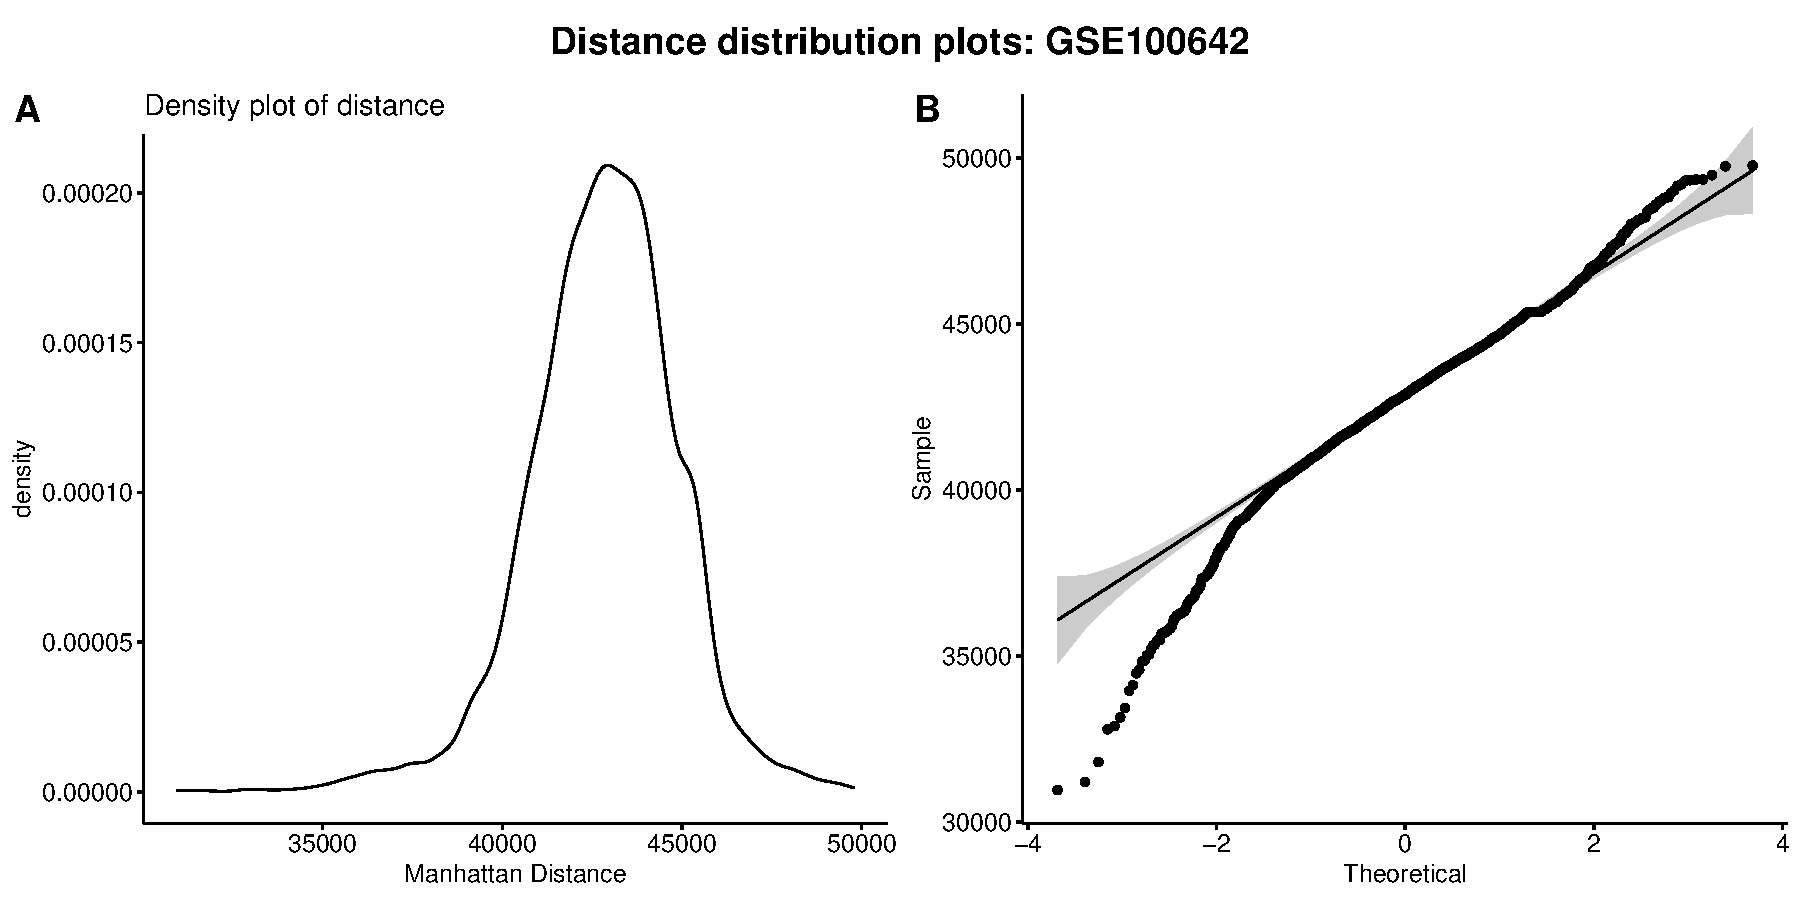
\includegraphics[width=\textwidth]{manhattan-distance_hist_GSE100642.pdf}
	\caption{Density and quantile-quantile plots for distances between samples in GSE100642. \textbf{A} Estimated density curve for distances. \textbf{B} Quantile-quantile plot between theoretical (standard normal) quantiles and sample distance quantiles.}
\end{figure}

\begin{figure}[H]
	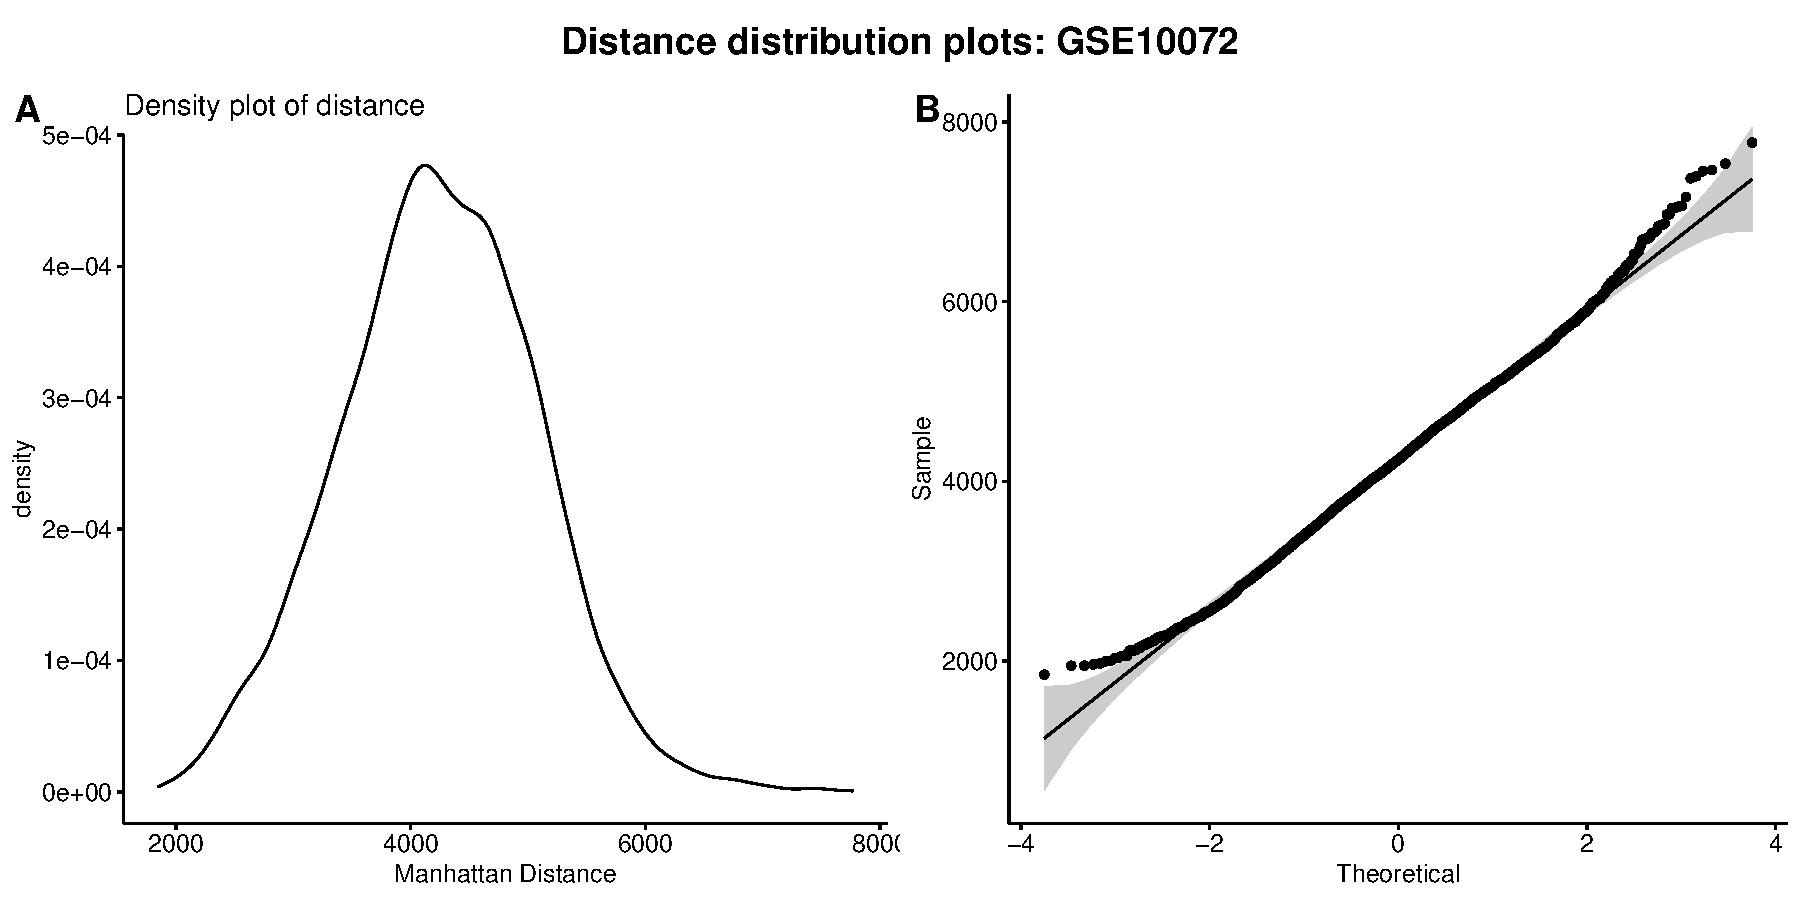
\includegraphics[width=\textwidth]{manhattan-distance_hist_GSE10072.pdf}
	\caption{Density and quantile-quantile plots for distances between samples in GSE10072. \textbf{A} Estimated density curve for distances. \textbf{B} Quantile-quantile plot between theoretical (standard normal) quantiles and sample distance quantiles.}
\end{figure}

\begin{figure}[H]
	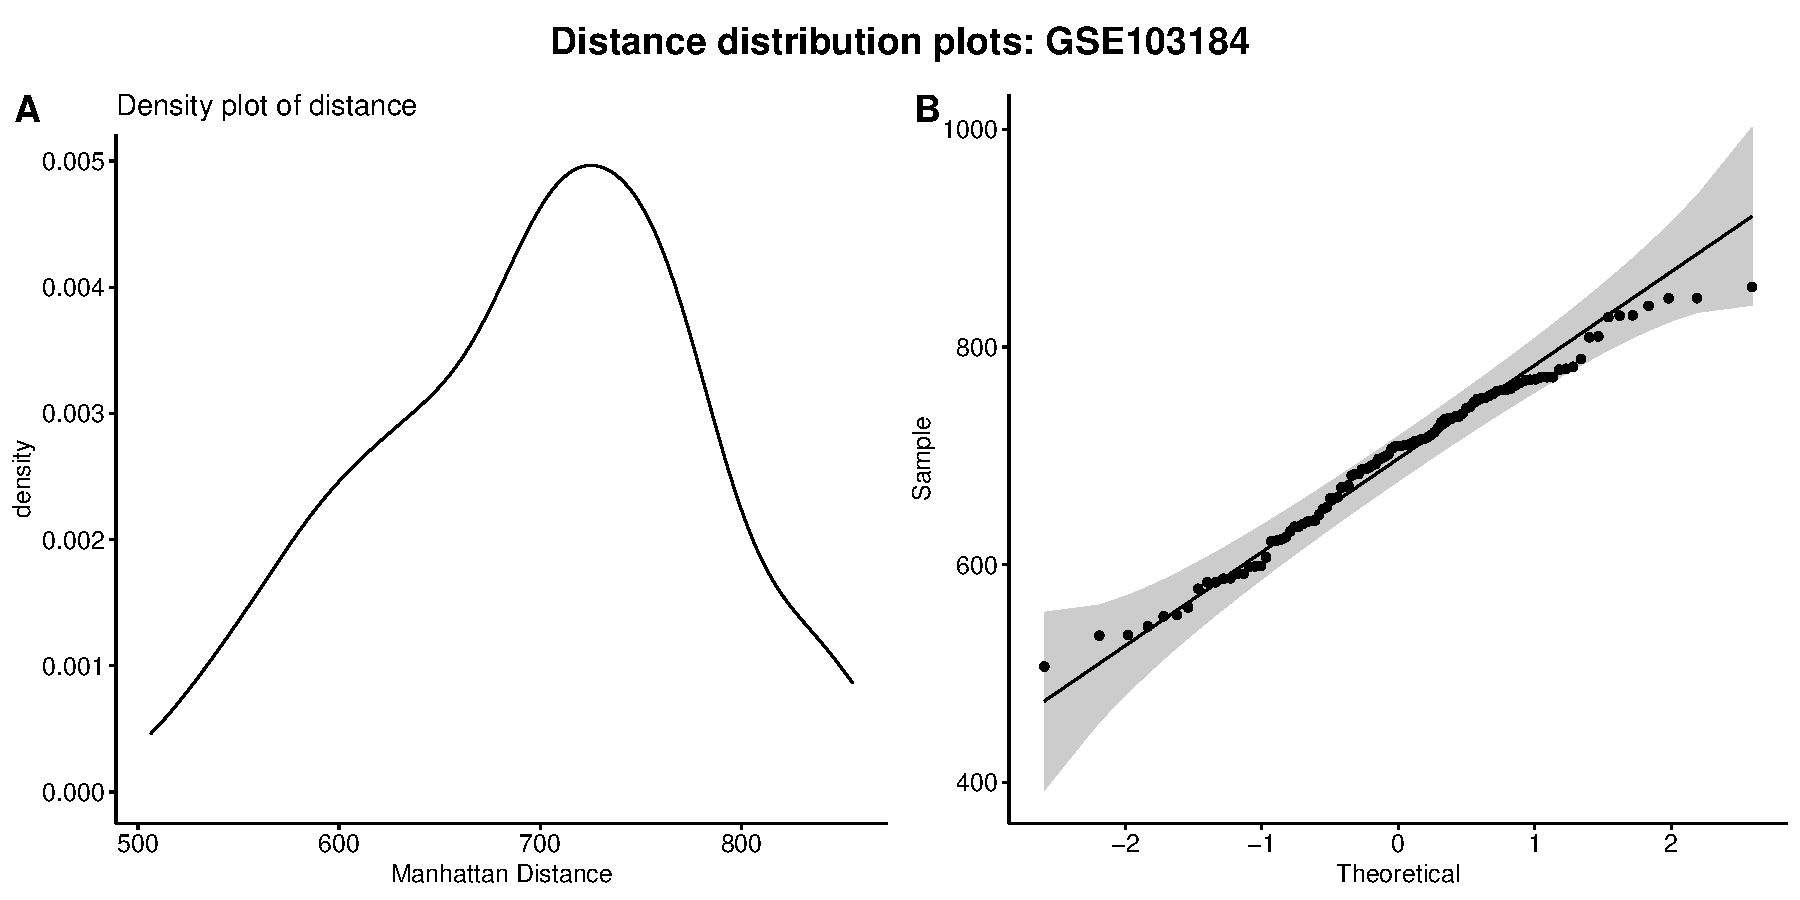
\includegraphics[width=\textwidth]{manhattan-distance_hist_GSE103184.pdf}
	\caption{Density and quantile-quantile plots for distances between samples in GSE103184. \textbf{A} Estimated density curve for distances. \textbf{B} Quantile-quantile plot between theoretical (standard normal) quantiles and sample distance quantiles.}
\end{figure}

\begin{figure}[H]
	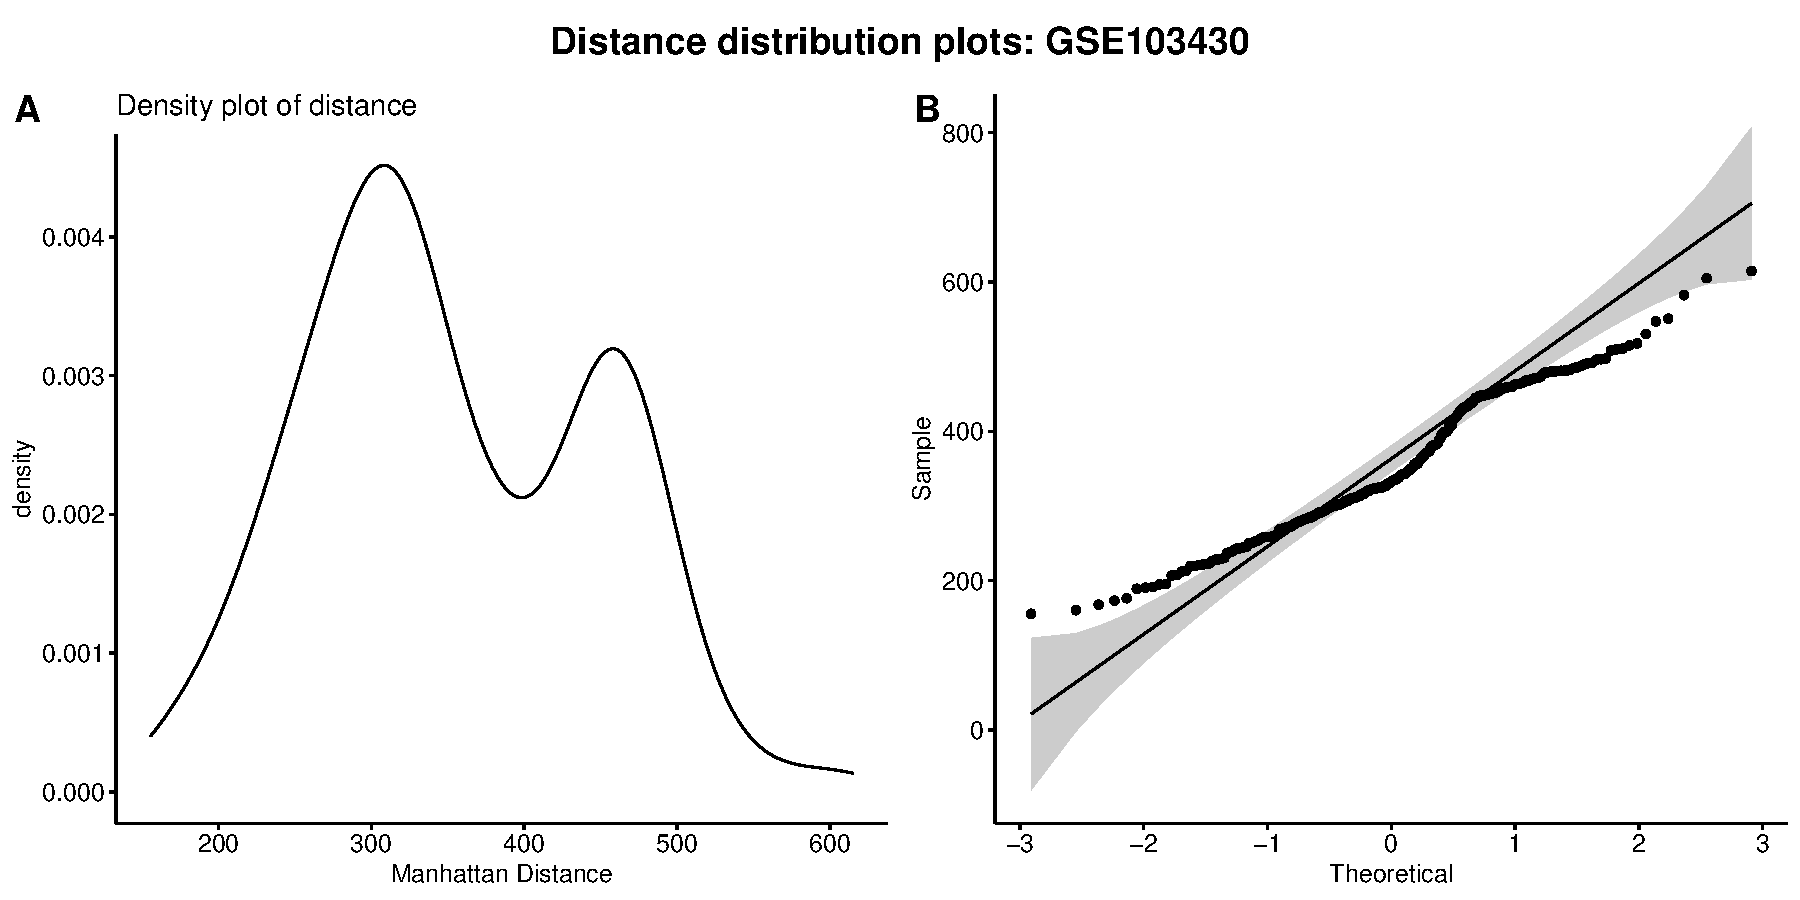
\includegraphics[width=\textwidth]{manhattan-distance_hist_GSE103430.pdf}
	\caption{Density and quantile-quantile plots for distances between samples in GSE103430. \textbf{A} Estimated density curve for distances. \textbf{B} Quantile-quantile plot between theoretical (standard normal) quantiles and sample distance quantiles.}
\end{figure}

\begin{figure}[H]
	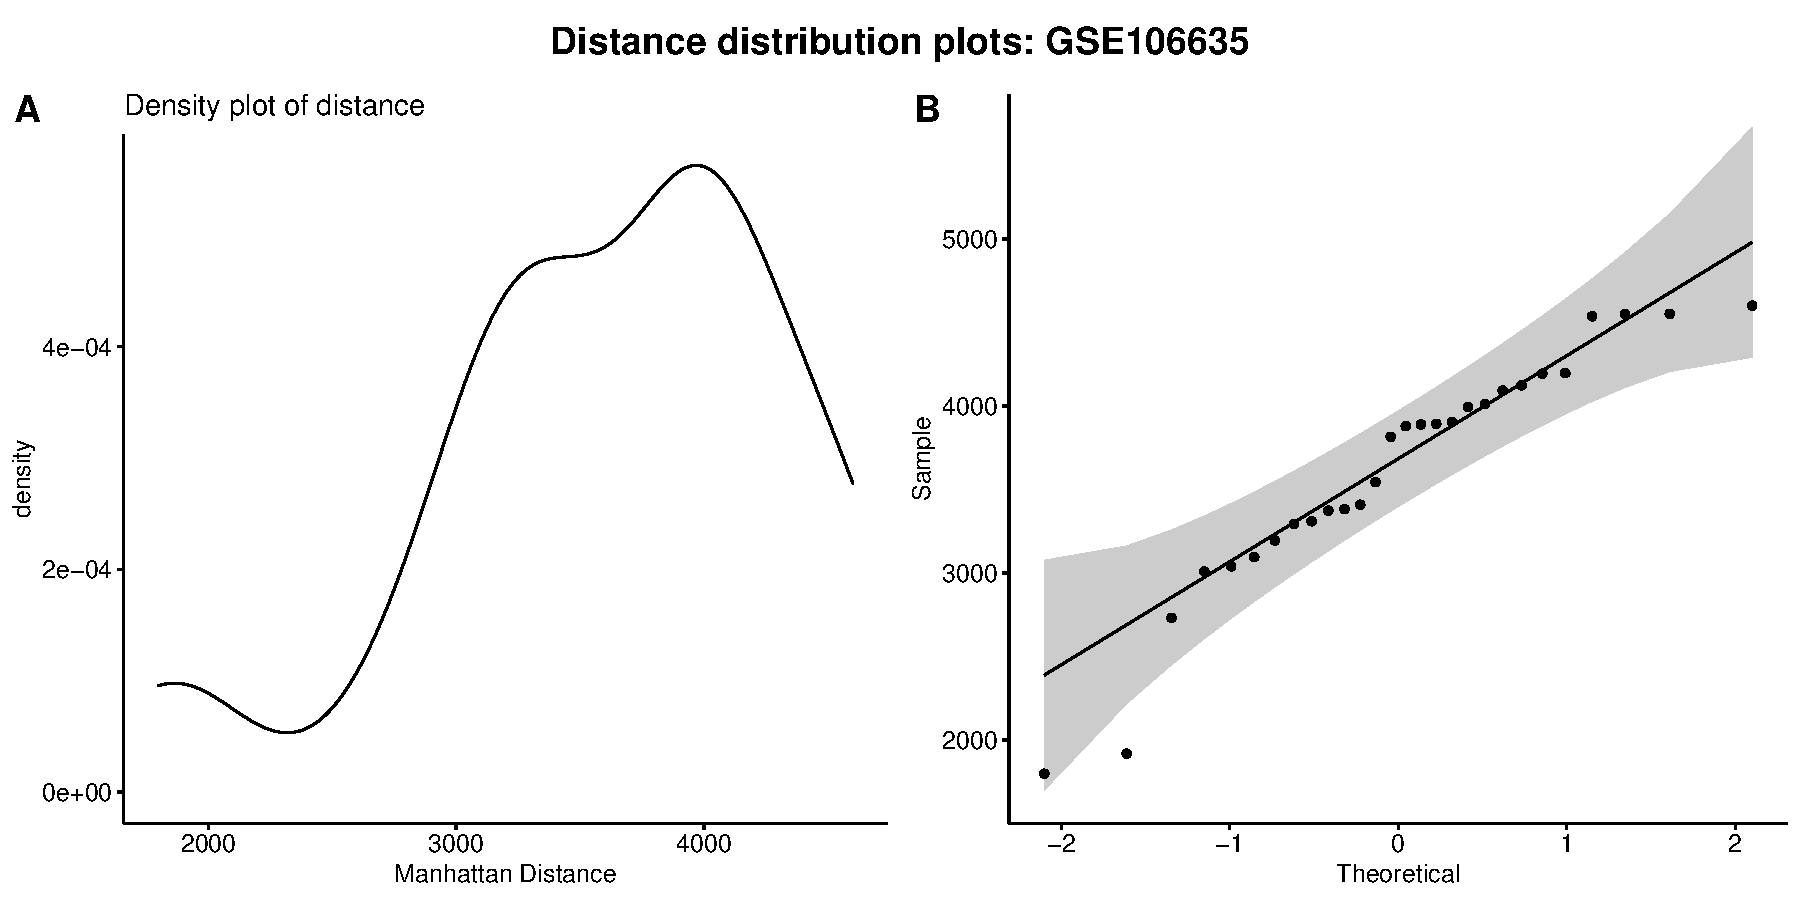
\includegraphics[width=\textwidth]{manhattan-distance_hist_GSE106635.pdf}
	\caption{Density and quantile-quantile plots for distances between samples in GSE106635. \textbf{A} Estimated density curve for distances. \textbf{B} Quantile-quantile plot between theoretical (standard normal) quantiles and sample distance quantiles.}
\end{figure}

\begin{figure}[H]
	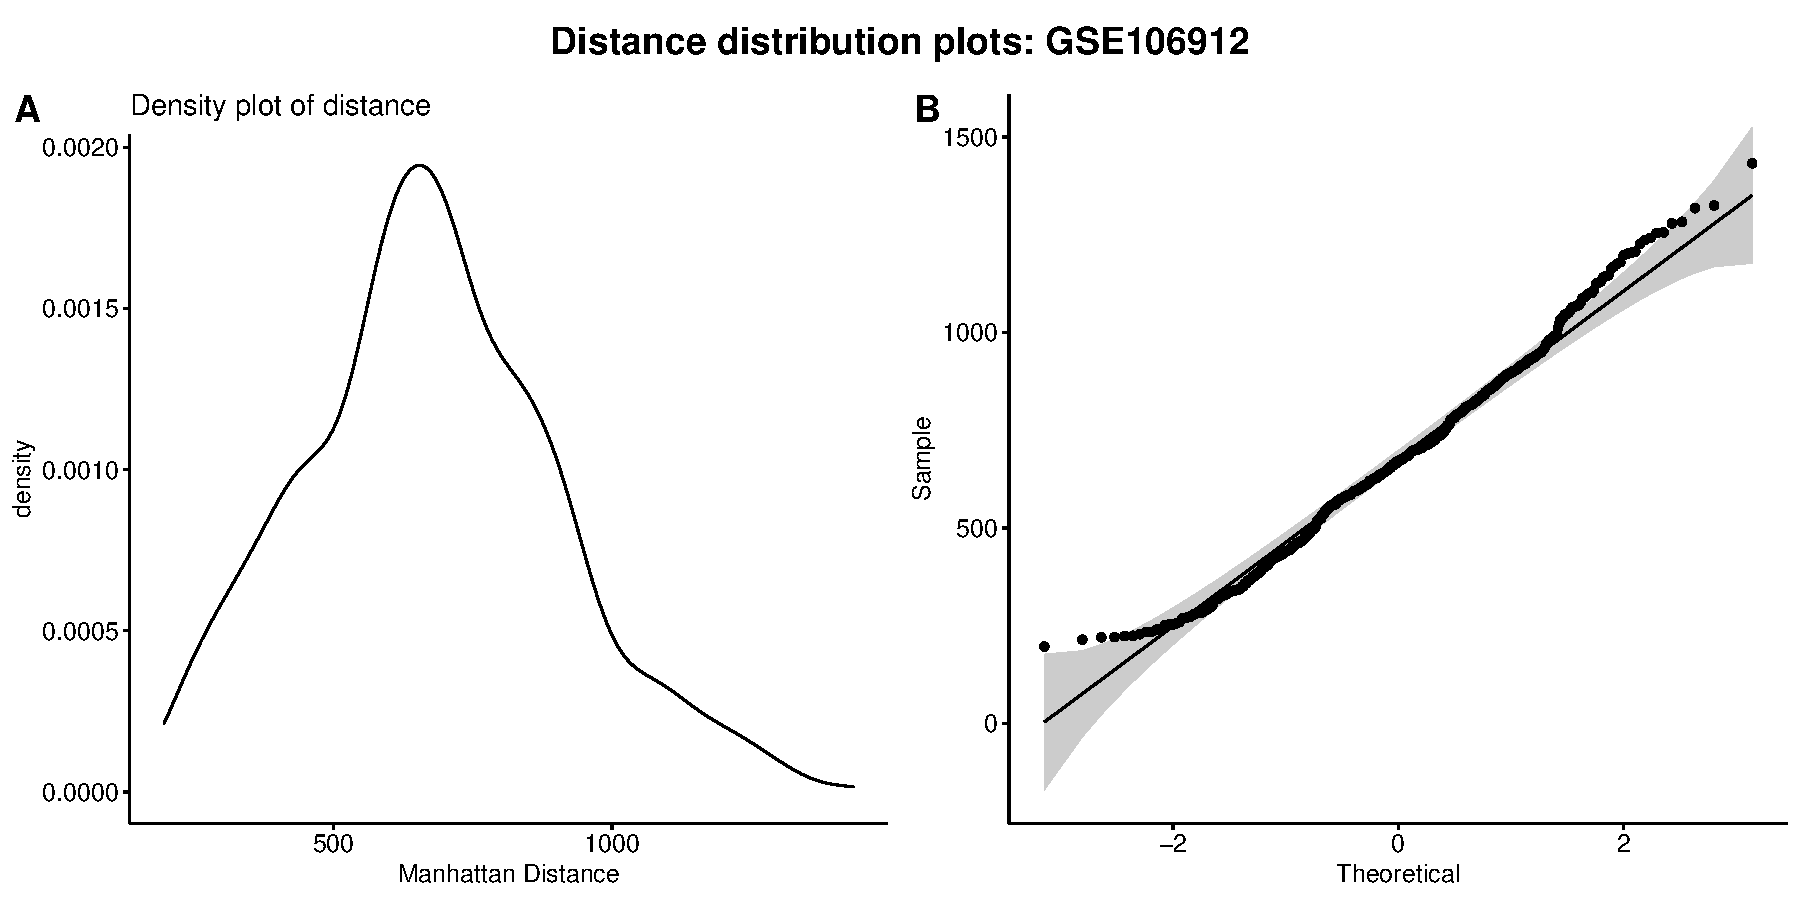
\includegraphics[width=\textwidth]{manhattan-distance_hist_GSE106912.pdf}
	\caption{Density and quantile-quantile plots for distances between samples in GSE106912. \textbf{A} Estimated density curve for distances. \textbf{B} Quantile-quantile plot between theoretical (standard normal) quantiles and sample distance quantiles.}
\end{figure}

\begin{figure}[H]
	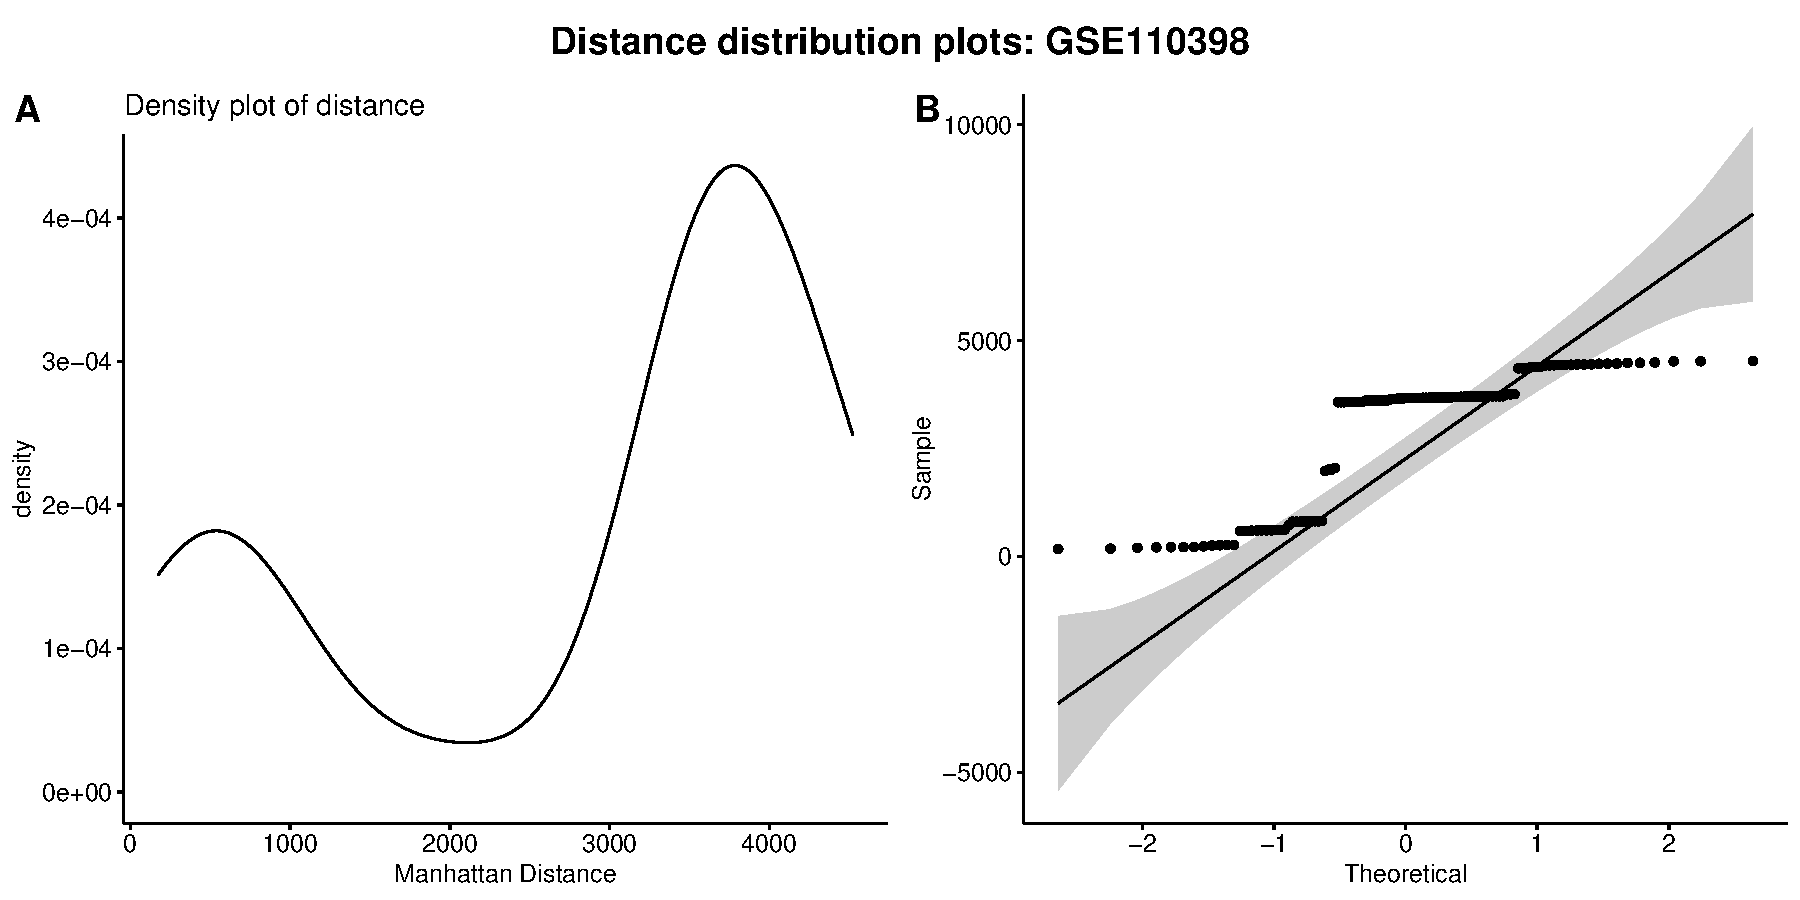
\includegraphics[width=\textwidth]{manhattan-distance_hist_GSE110398.pdf}
	\caption{Density and quantile-quantile plots for distances between samples in GSE110398. \textbf{A} Estimated density curve for distances. \textbf{B} Quantile-quantile plot between theoretical (standard normal) quantiles and sample distance quantiles.}
\end{figure}

\begin{figure}[H]
	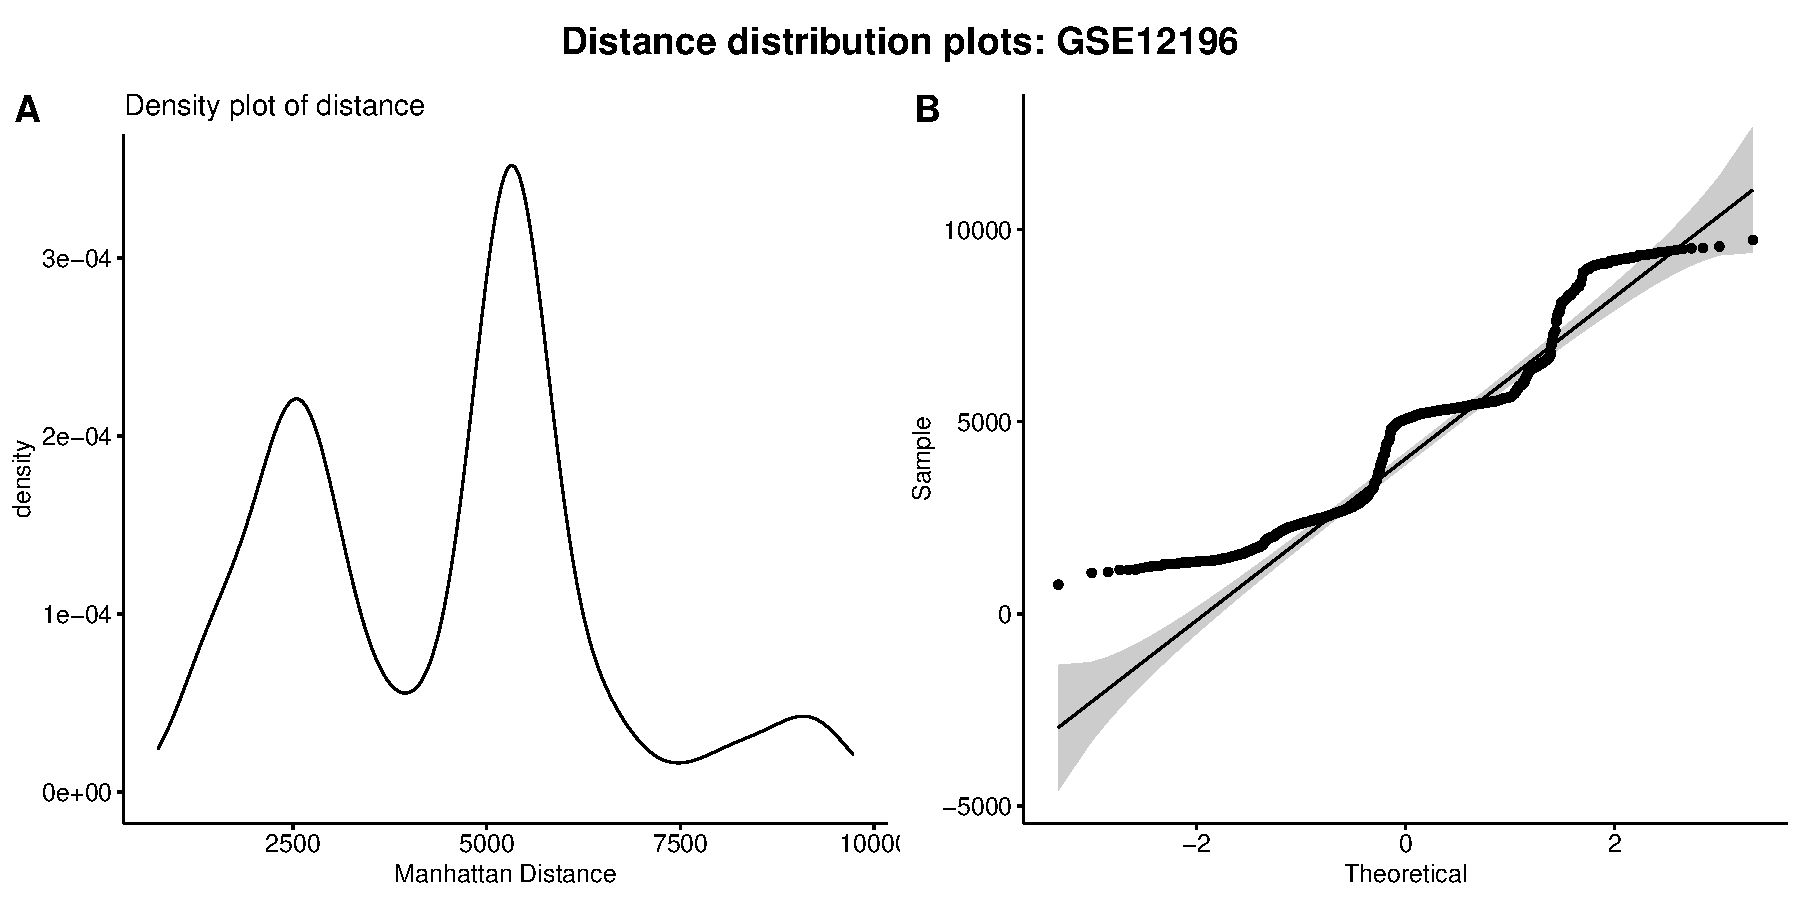
\includegraphics[width=\textwidth]{manhattan-distance_hist_GSE12196.pdf}
	\caption{Density and quantile-quantile plots for distances between samples in GSE12196. \textbf{A} Estimated density curve for distances. \textbf{B} Quantile-quantile plot between theoretical (standard normal) quantiles and sample distance quantiles.}
\end{figure}

\begin{figure}[H]
	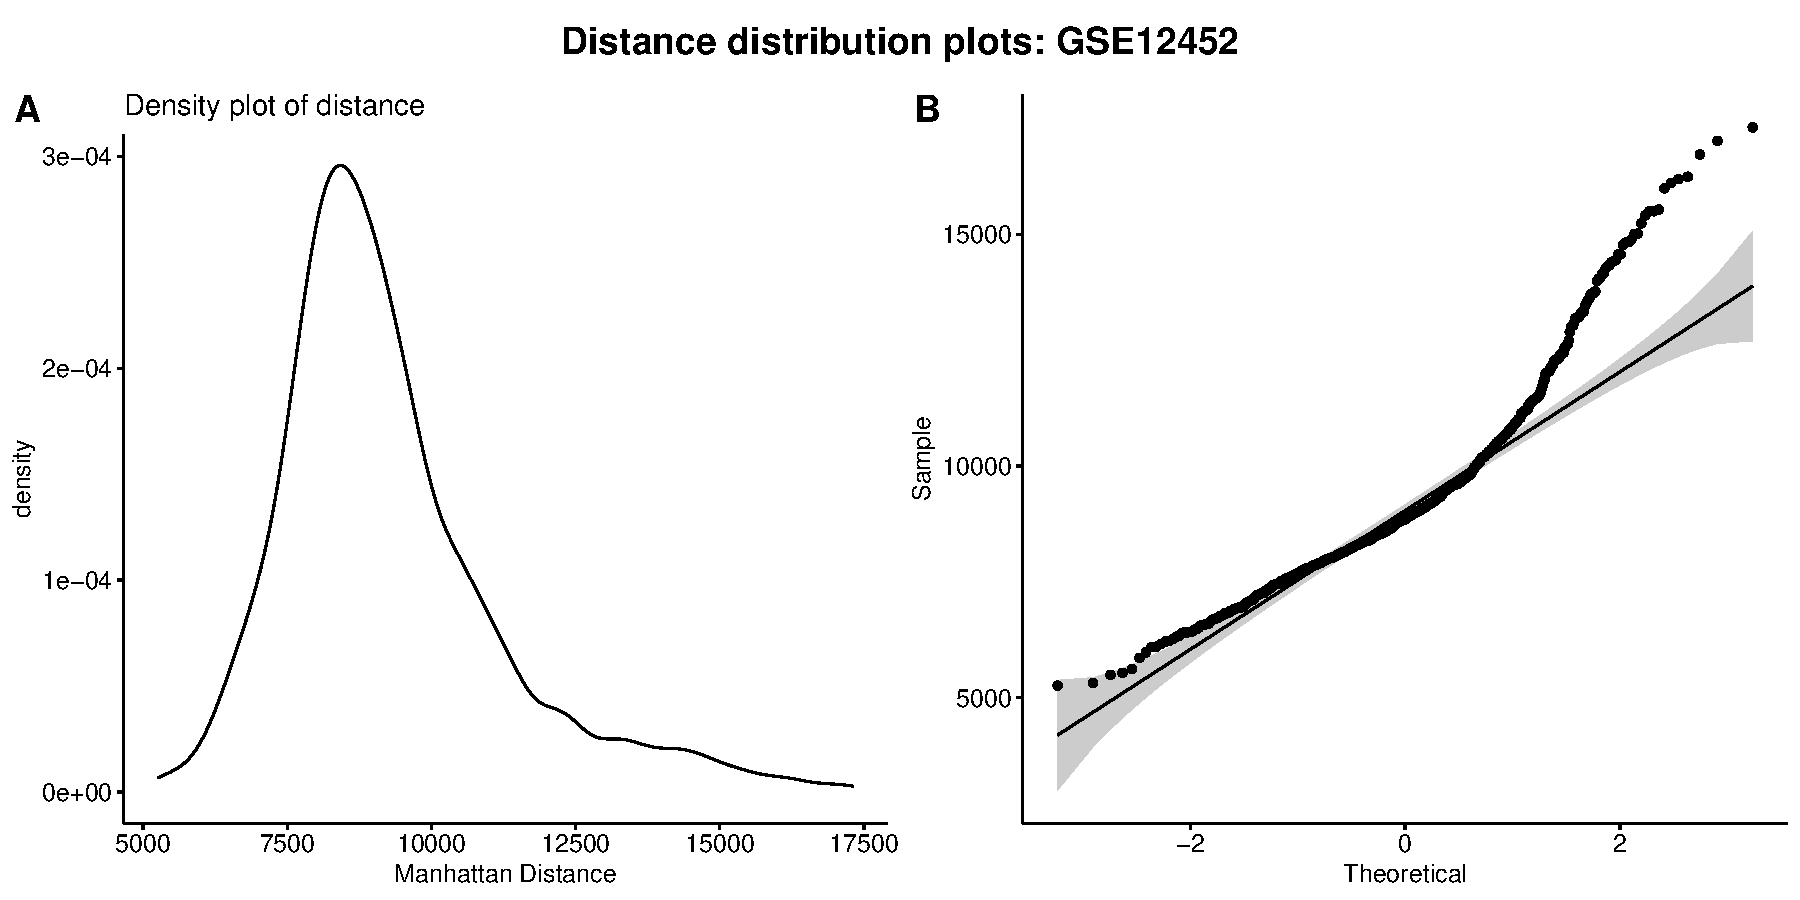
\includegraphics[width=\textwidth]{manhattan-distance_hist_GSE12452.pdf}
	\caption{Density and quantile-quantile plots for distances between samples in GSE12452. \textbf{A} Estimated density curve for distances. \textbf{B} Quantile-quantile plot between theoretical (standard normal) quantiles and sample distance quantiles.}
\end{figure}

\begin{figure}[H]
	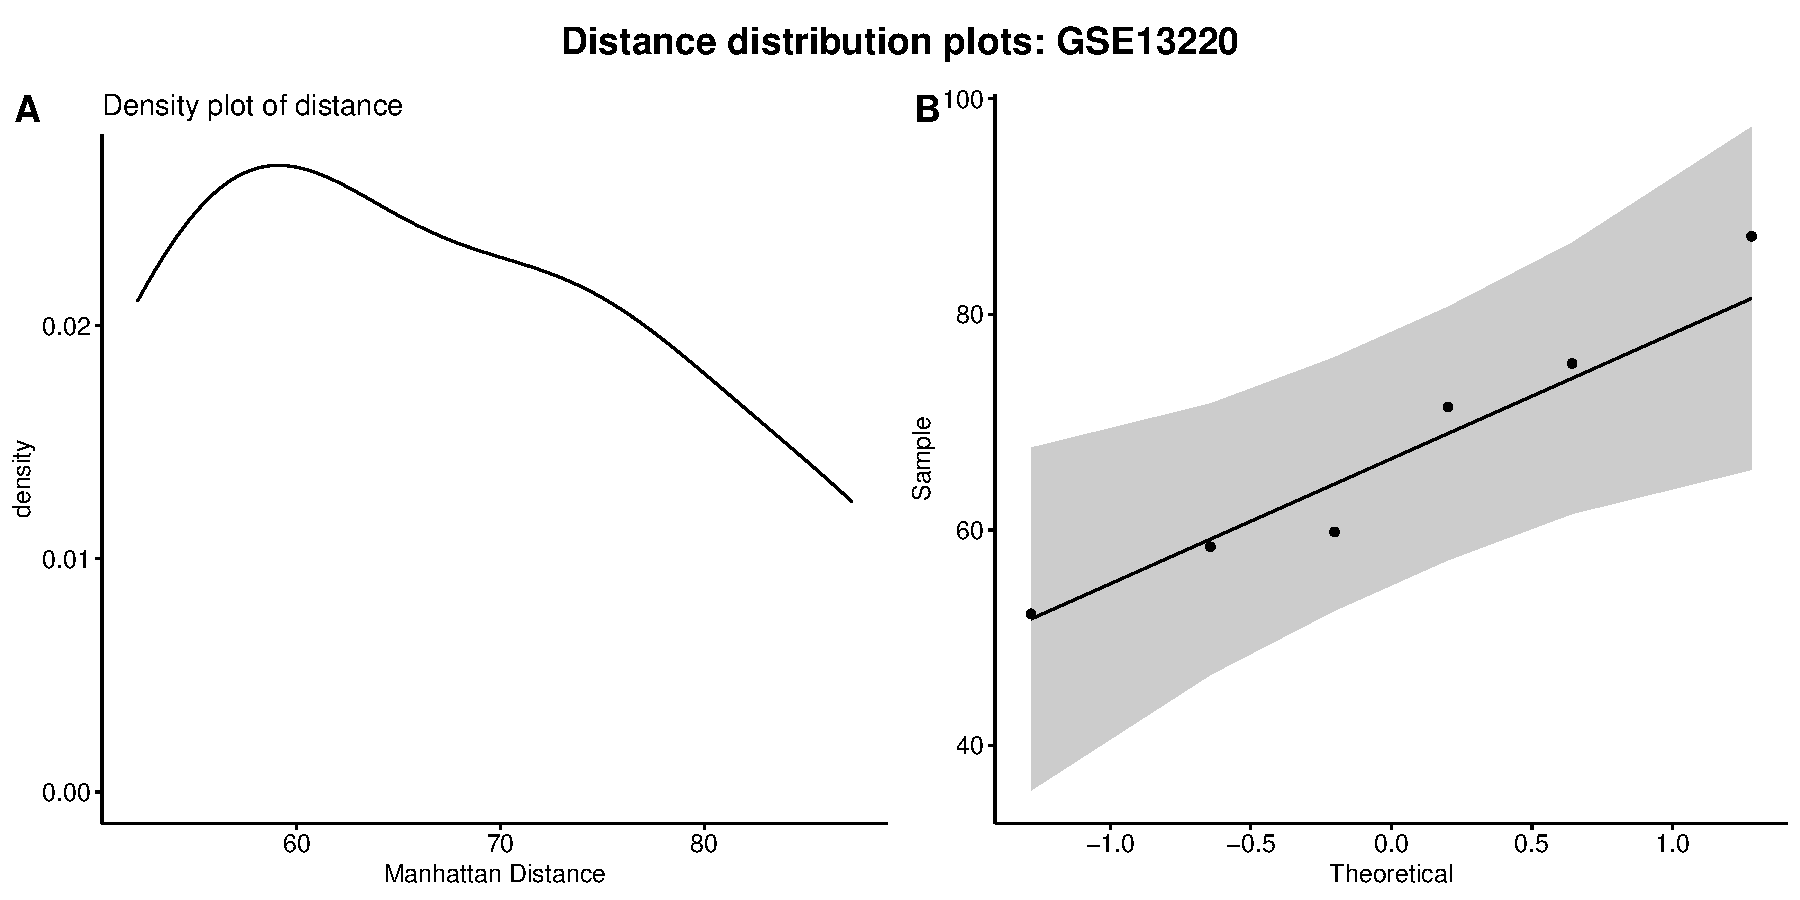
\includegraphics[width=\textwidth]{manhattan-distance_hist_GSE13220.pdf}
	\caption{Density and quantile-quantile plots for distances between samples in GSE13220. \textbf{A} Estimated density curve for distances. \textbf{B} Quantile-quantile plot between theoretical (standard normal) quantiles and sample distance quantiles.}
\end{figure}

\begin{figure}[H]
	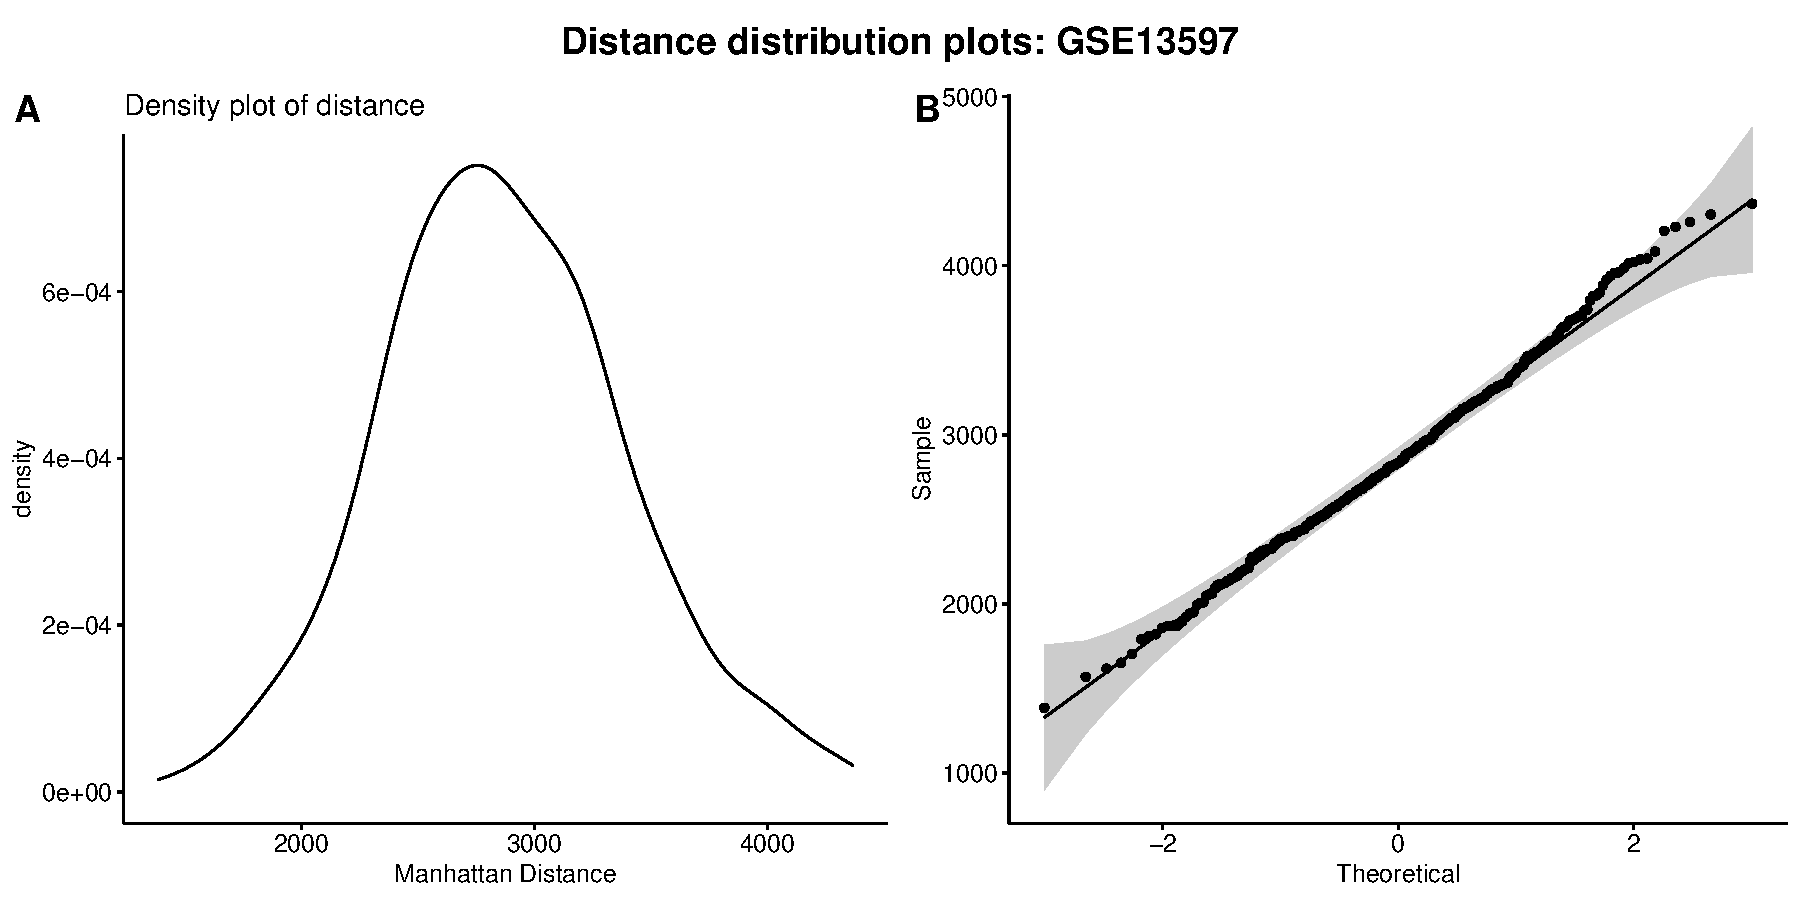
\includegraphics[width=\textwidth]{manhattan-distance_hist_GSE13597.pdf}
	\caption{Density and quantile-quantile plots for distances between samples in GSE13597. \textbf{A} Estimated density curve for distances. \textbf{B} Quantile-quantile plot between theoretical (standard normal) quantiles and sample distance quantiles.}
\end{figure}

\begin{figure}[H]
	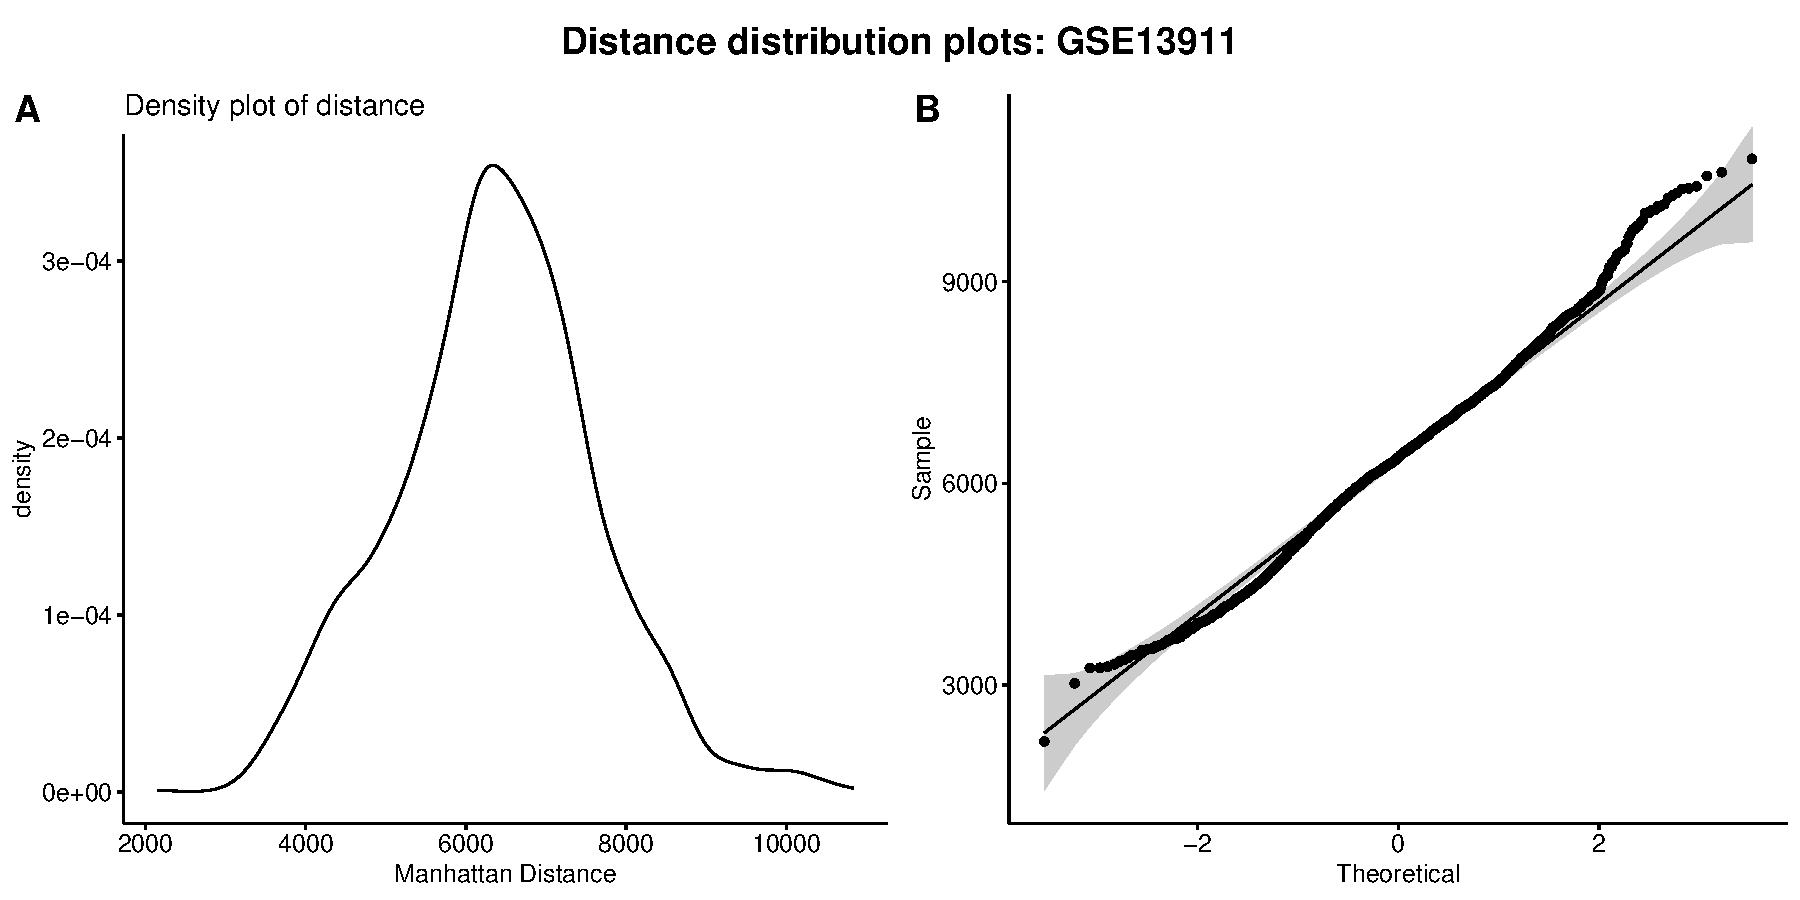
\includegraphics[width=\textwidth]{manhattan-distance_hist_GSE13911.pdf}
	\caption{Density and quantile-quantile plots for distances between samples in GSE13911. \textbf{A} Estimated density curve for distances. \textbf{B} Quantile-quantile plot between theoretical (standard normal) quantiles and sample distance quantiles.}
\end{figure}

\begin{figure}[H]
	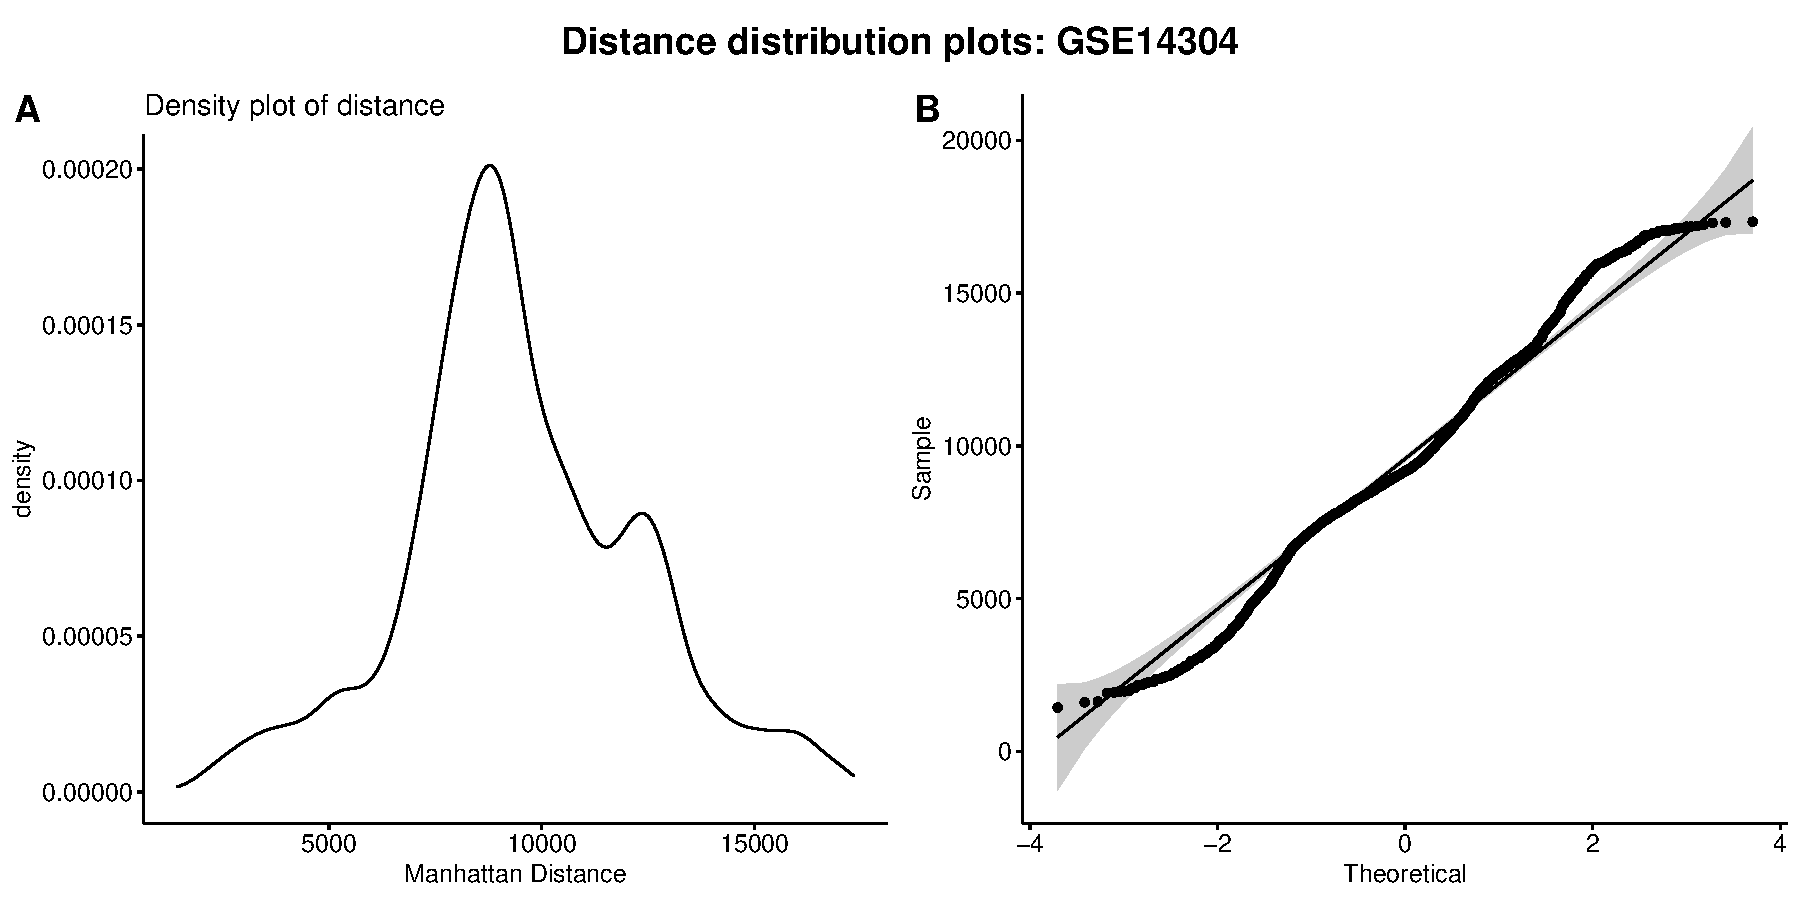
\includegraphics[width=\textwidth]{manhattan-distance_hist_GSE14304.pdf}
	\caption{Density and quantile-quantile plots for distances between samples in GSE14304. \textbf{A} Estimated density curve for distances. \textbf{B} Quantile-quantile plot between theoretical (standard normal) quantiles and sample distance quantiles.}
\end{figure}

\begin{figure}[H]
	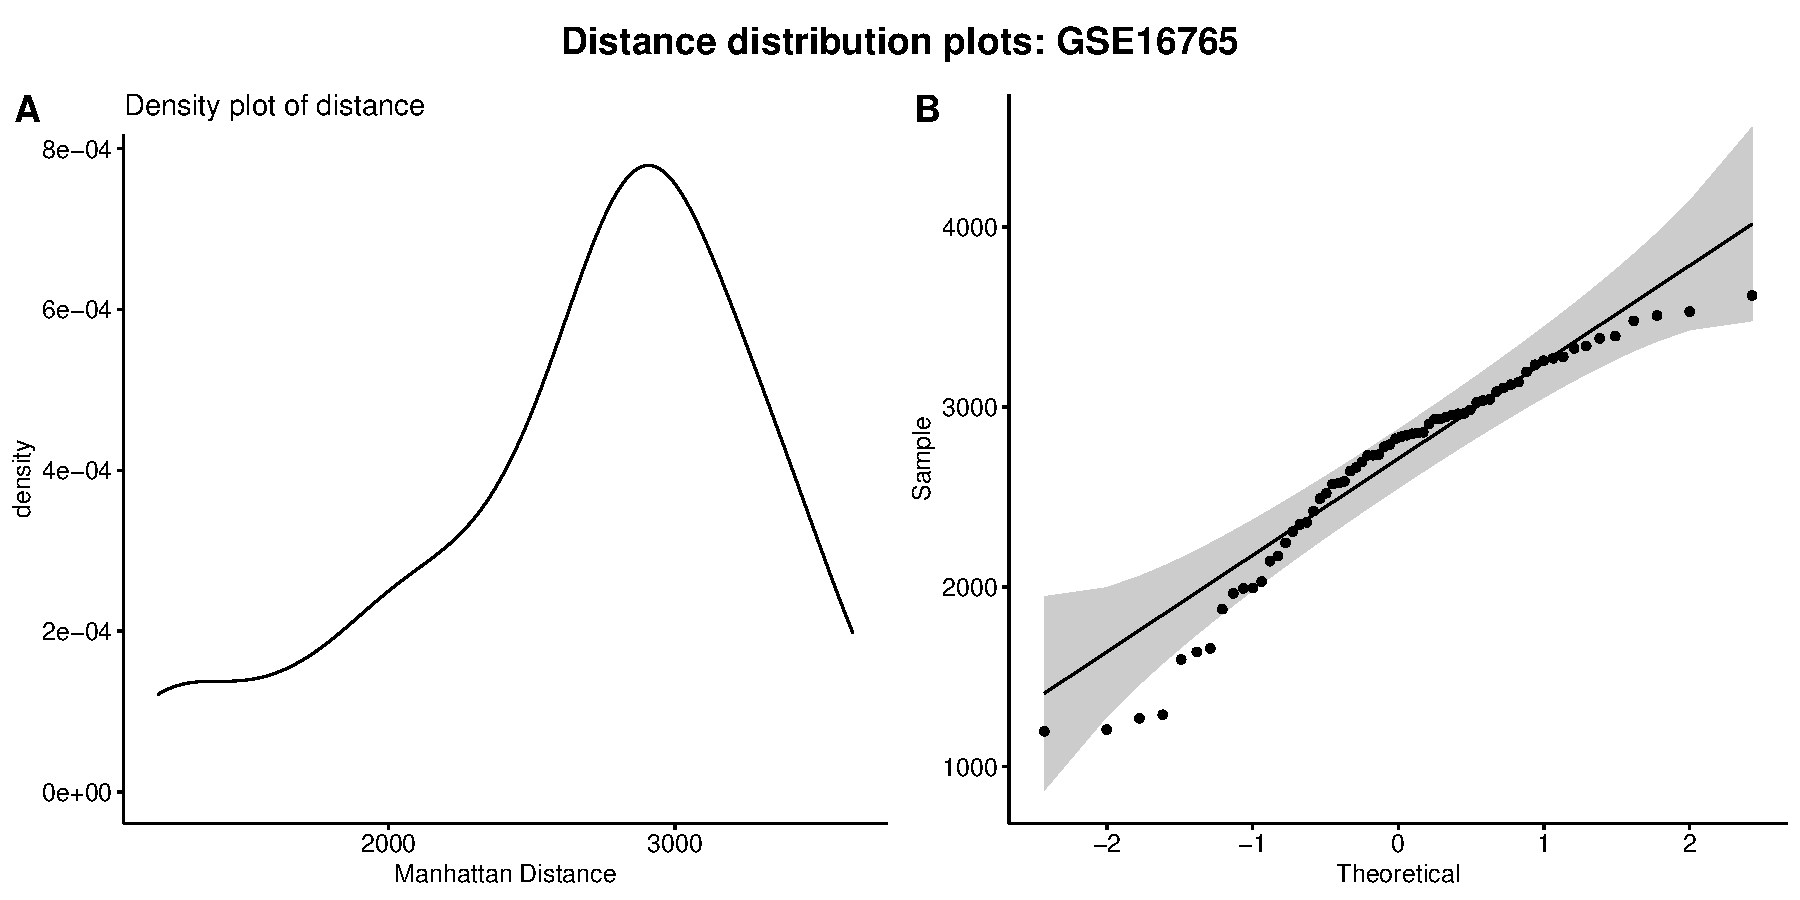
\includegraphics[width=\textwidth]{manhattan-distance_hist_GSE16765.pdf}
	\caption{Density and quantile-quantile plots for distances between samples in GSE16765. \textbf{A} Estimated density curve for distances. \textbf{B} Quantile-quantile plot between theoretical (standard normal) quantiles and sample distance quantiles.}
\end{figure}

\begin{figure}[H]
	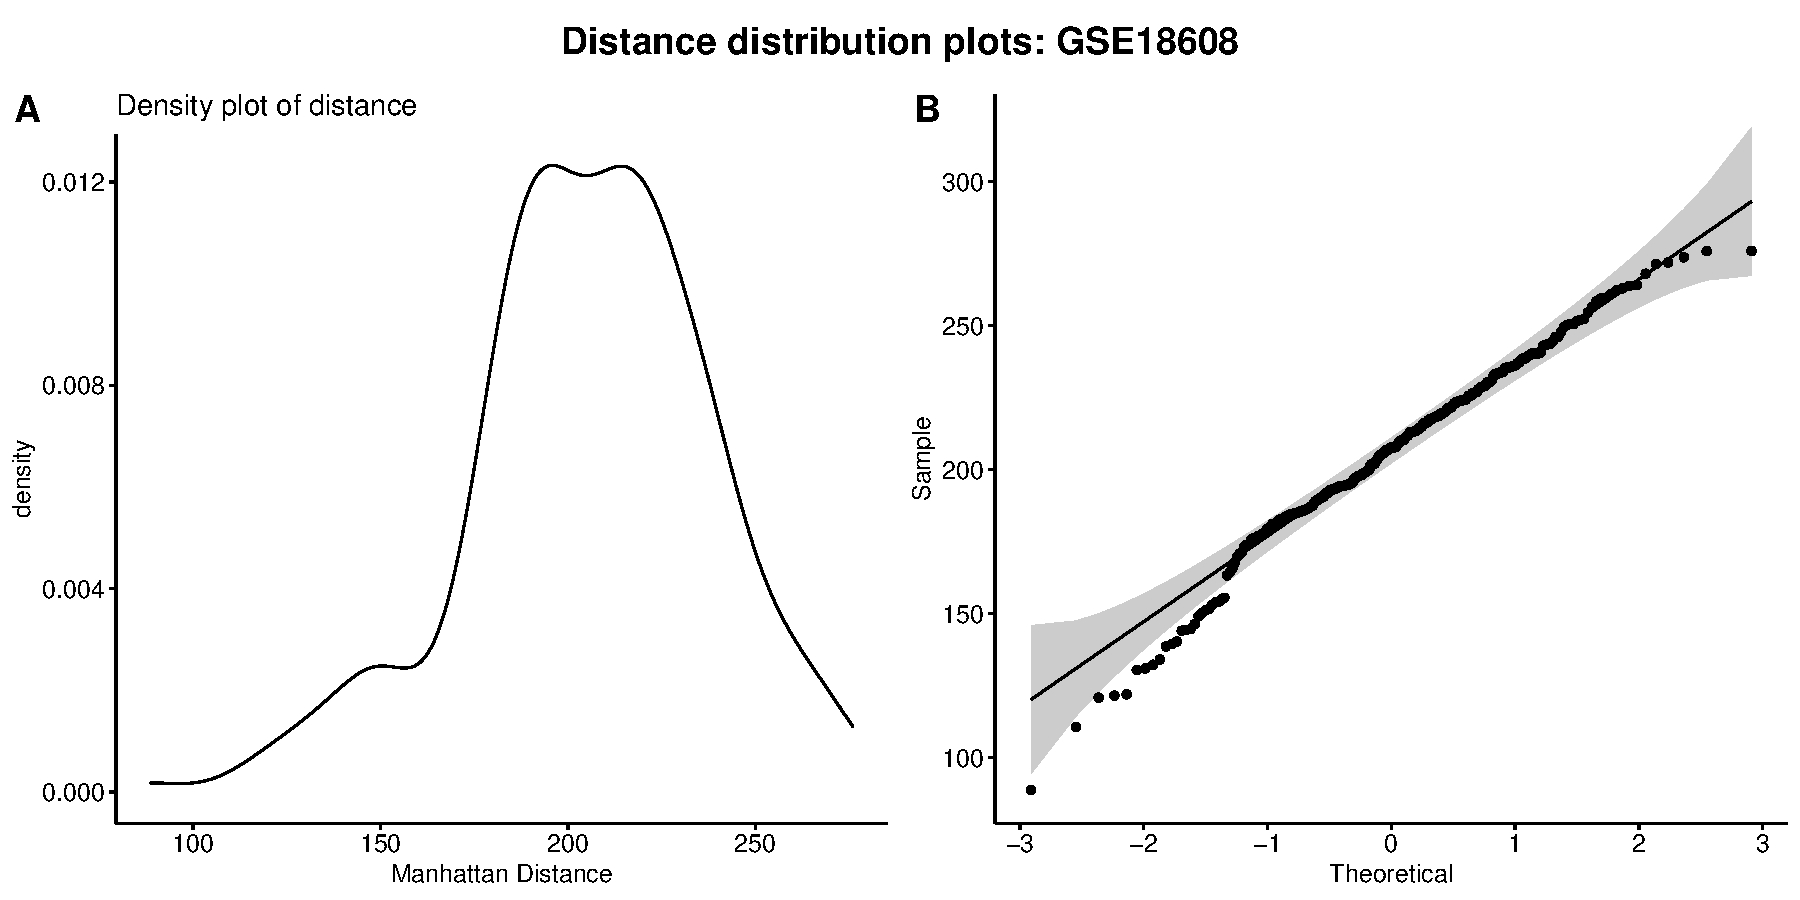
\includegraphics[width=\textwidth]{manhattan-distance_hist_GSE18608.pdf}
	\caption{Density and quantile-quantile plots for distances between samples in GSE18608. \textbf{A} Estimated density curve for distances. \textbf{B} Quantile-quantile plot between theoretical (standard normal) quantiles and sample distance quantiles.}
\end{figure}

\begin{figure}[H]
	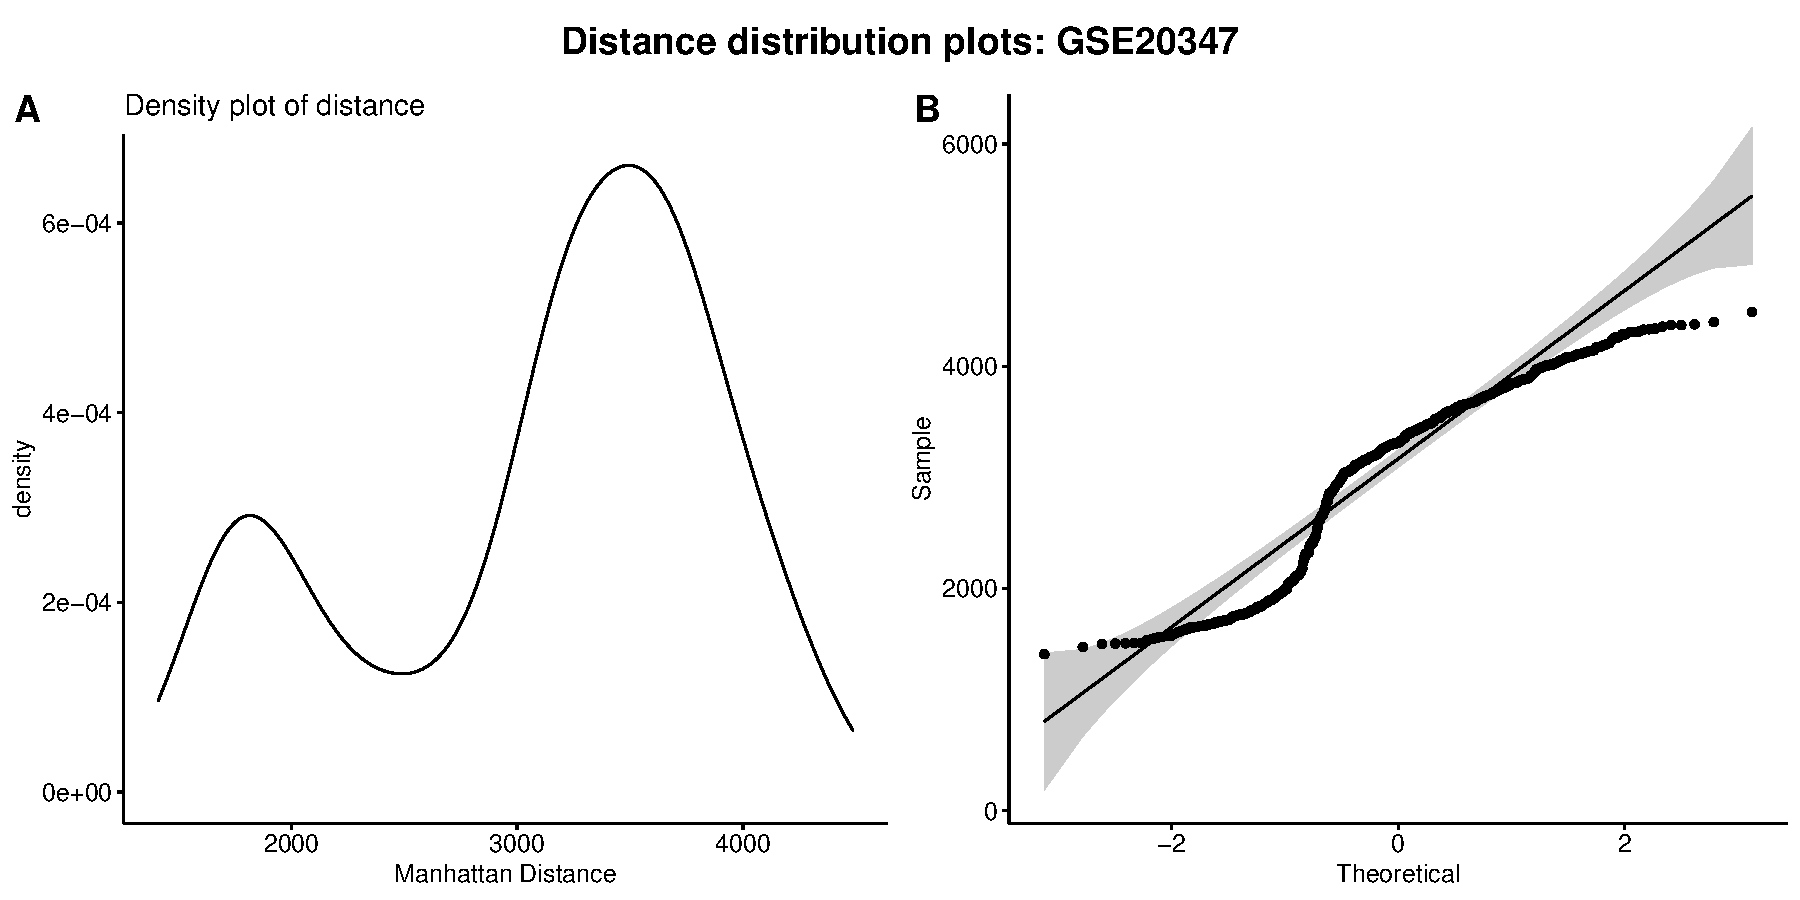
\includegraphics[width=\textwidth]{manhattan-distance_hist_GSE20347.pdf}
	\caption{Density and quantile-quantile plots for distances between samples in GSE20347. \textbf{A} Estimated density curve for distances. \textbf{B} Quantile-quantile plot between theoretical (standard normal) quantiles and sample distance quantiles.}
\end{figure}

\begin{figure}[H]
	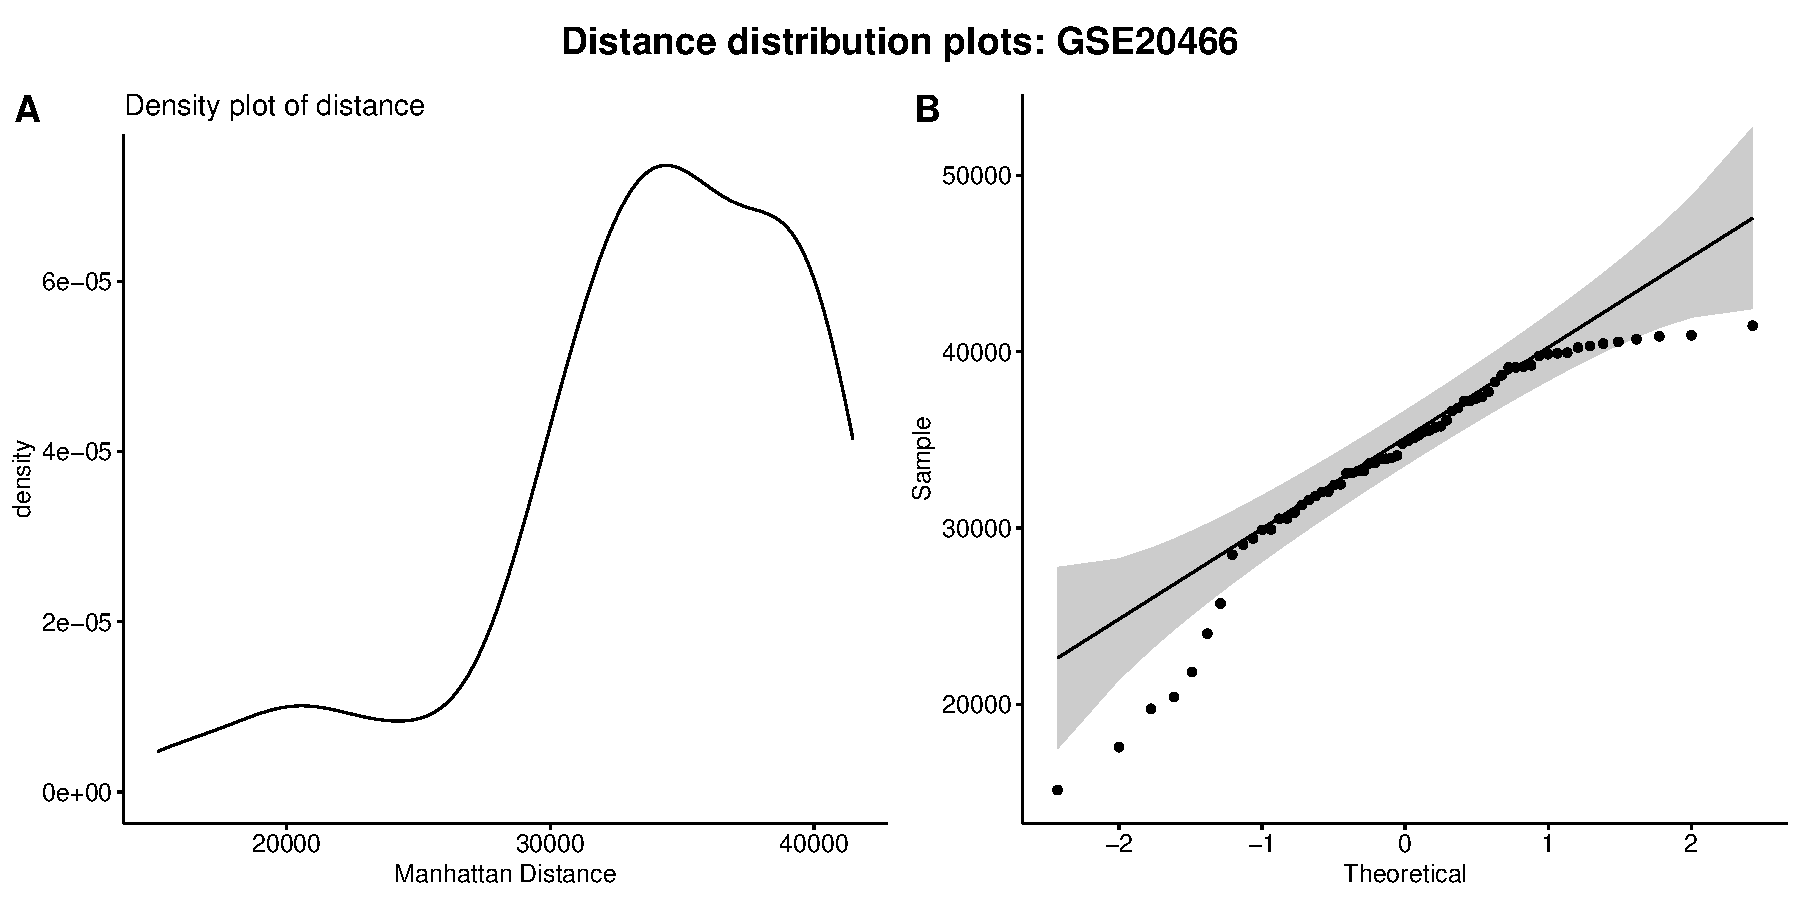
\includegraphics[width=\textwidth]{manhattan-distance_hist_GSE20466.pdf}
	\caption{Density and quantile-quantile plots for distances between samples in GSE20466. \textbf{A} Estimated density curve for distances. \textbf{B} Quantile-quantile plot between theoretical (standard normal) quantiles and sample distance quantiles.}
\end{figure}

\begin{figure}[H]
	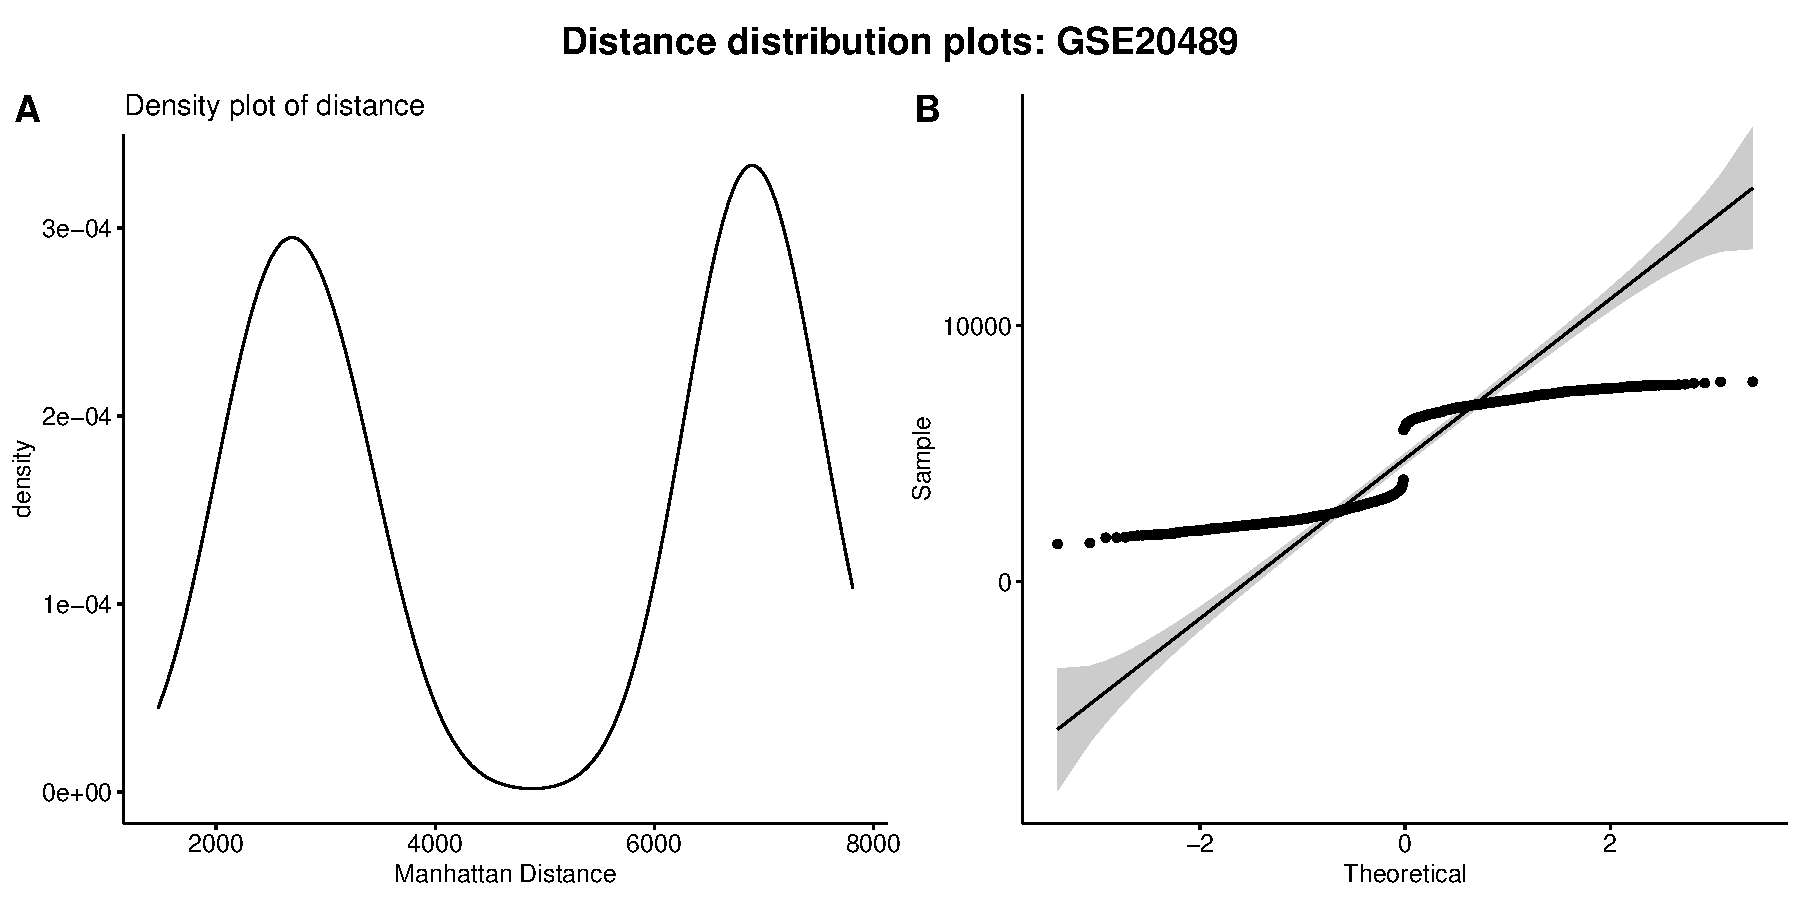
\includegraphics[width=\textwidth]{manhattan-distance_hist_GSE20489.pdf}
	\caption{Density and quantile-quantile plots for distances between samples in GSE20489. \textbf{A} Estimated density curve for distances. \textbf{B} Quantile-quantile plot between theoretical (standard normal) quantiles and sample distance quantiles.}
\end{figure}

\begin{figure}[H]
	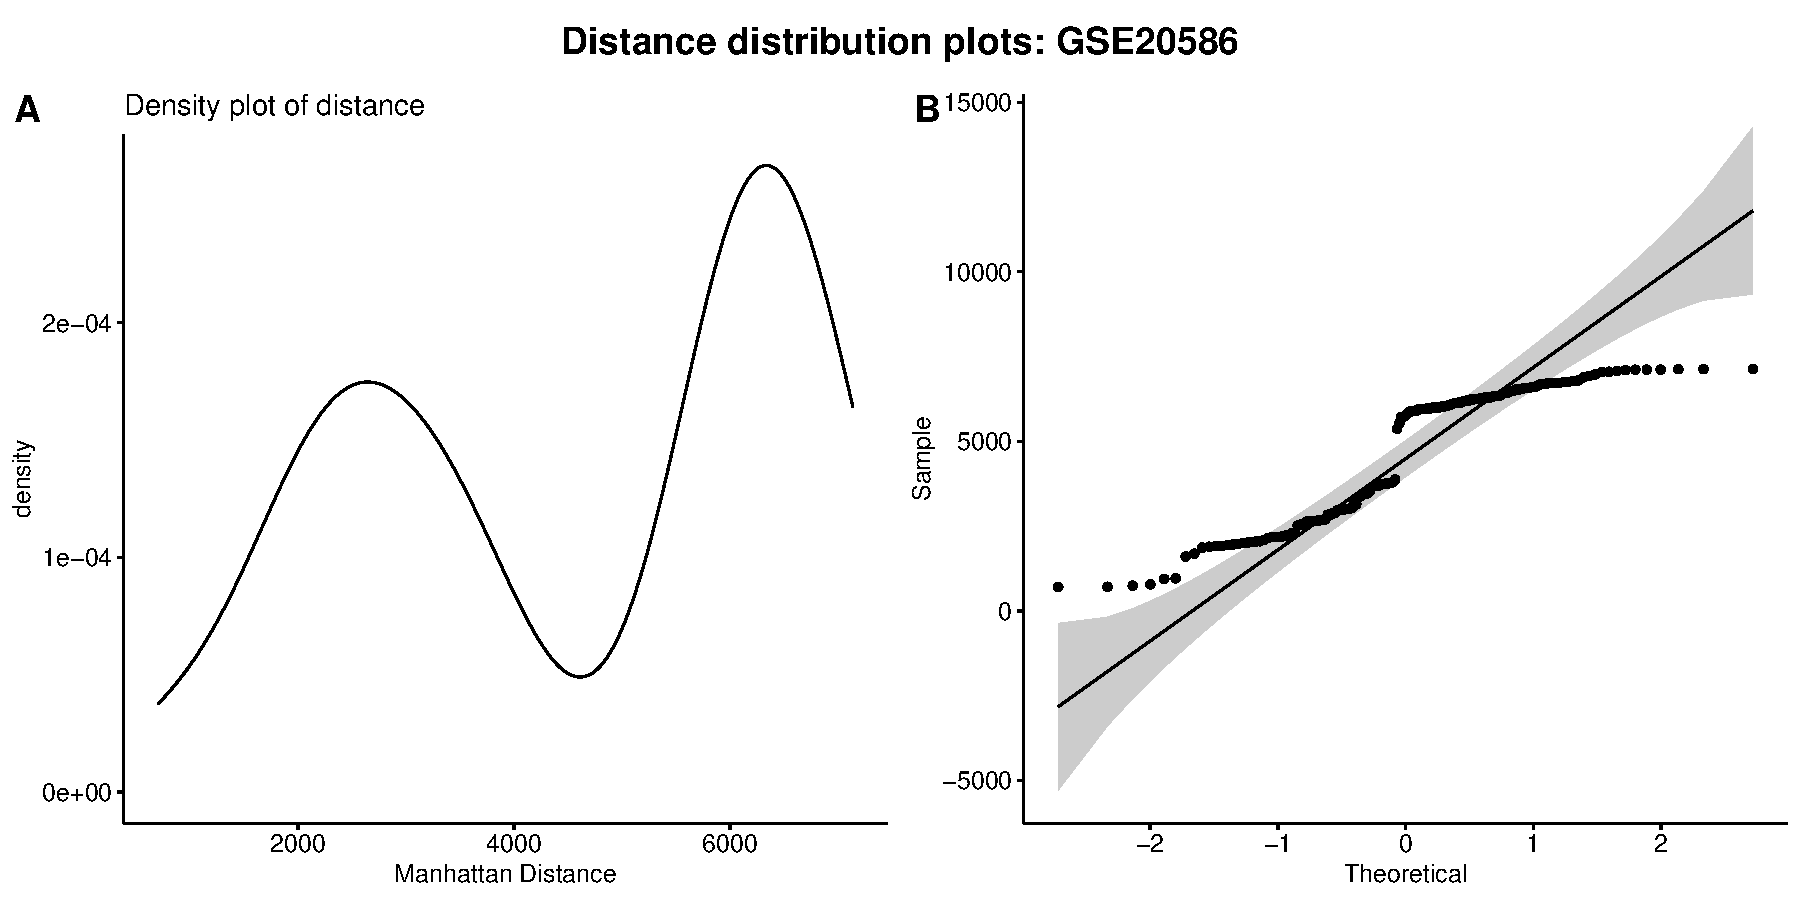
\includegraphics[width=\textwidth]{manhattan-distance_hist_GSE20586.pdf}
	\caption{Density and quantile-quantile plots for distances between samples in GSE20586. \textbf{A} Estimated density curve for distances. \textbf{B} Quantile-quantile plot between theoretical (standard normal) quantiles and sample distance quantiles.}
\end{figure}

\begin{figure}[H]
	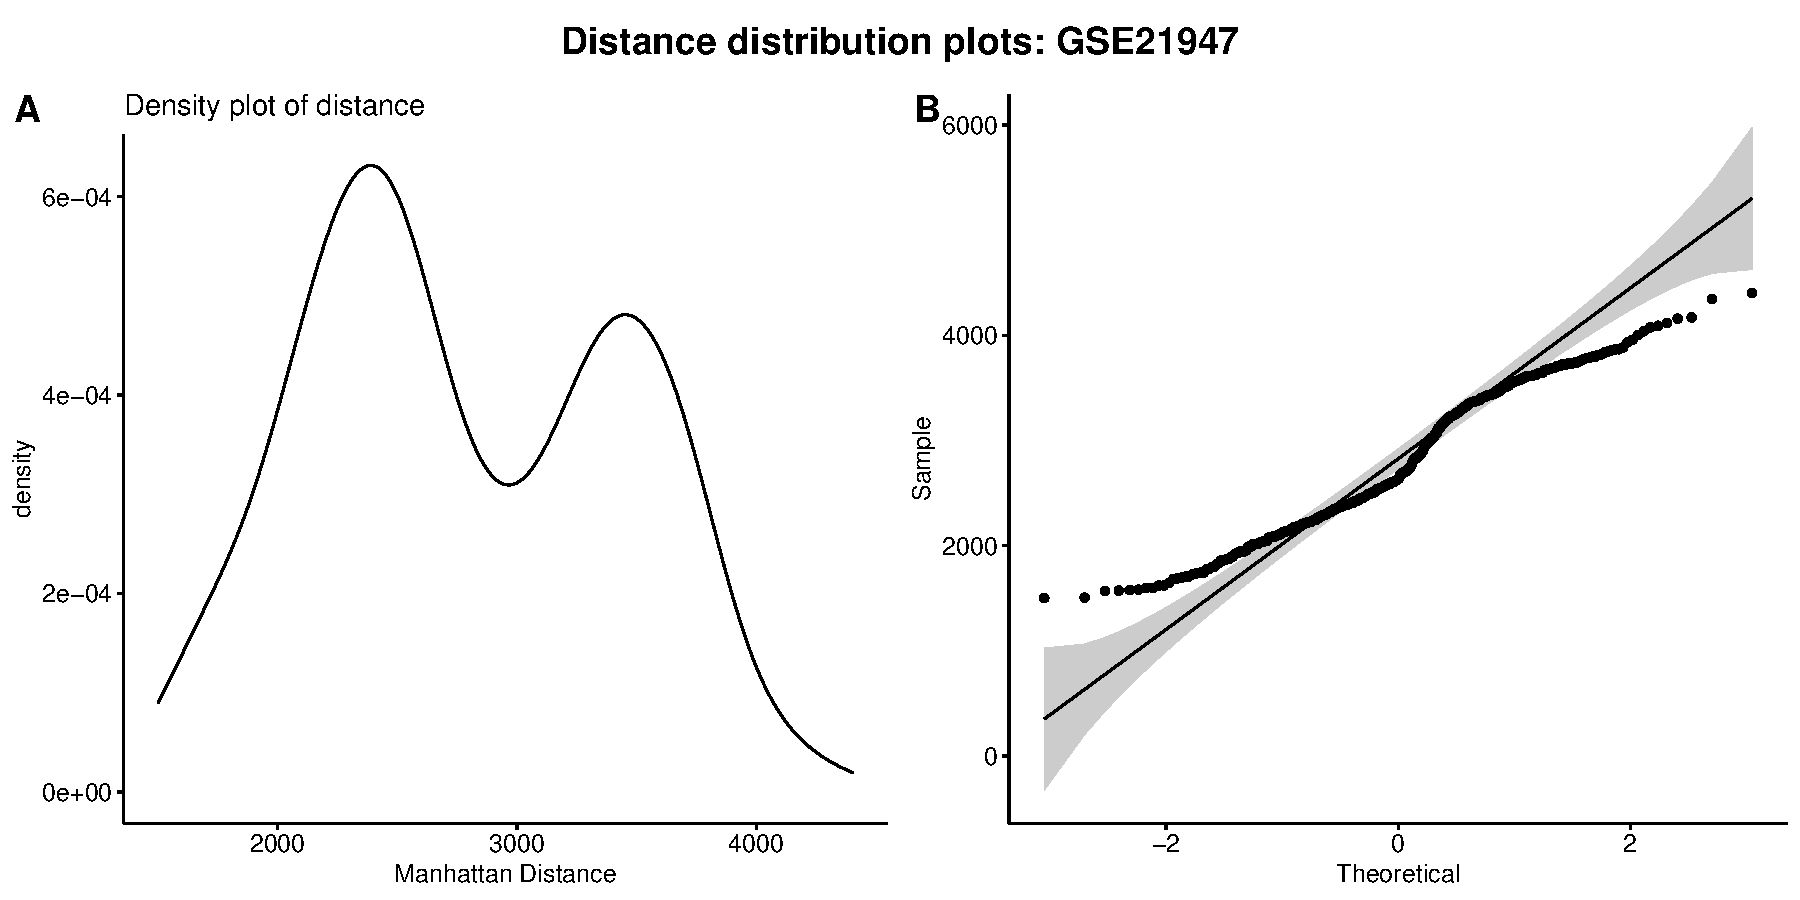
\includegraphics[width=\textwidth]{manhattan-distance_hist_GSE21947.pdf}
	\caption{Density and quantile-quantile plots for distances between samples in GSE21947. \textbf{A} Estimated density curve for distances. \textbf{B} Quantile-quantile plot between theoretical (standard normal) quantiles and sample distance quantiles.}
\end{figure}

\begin{figure}[H]
	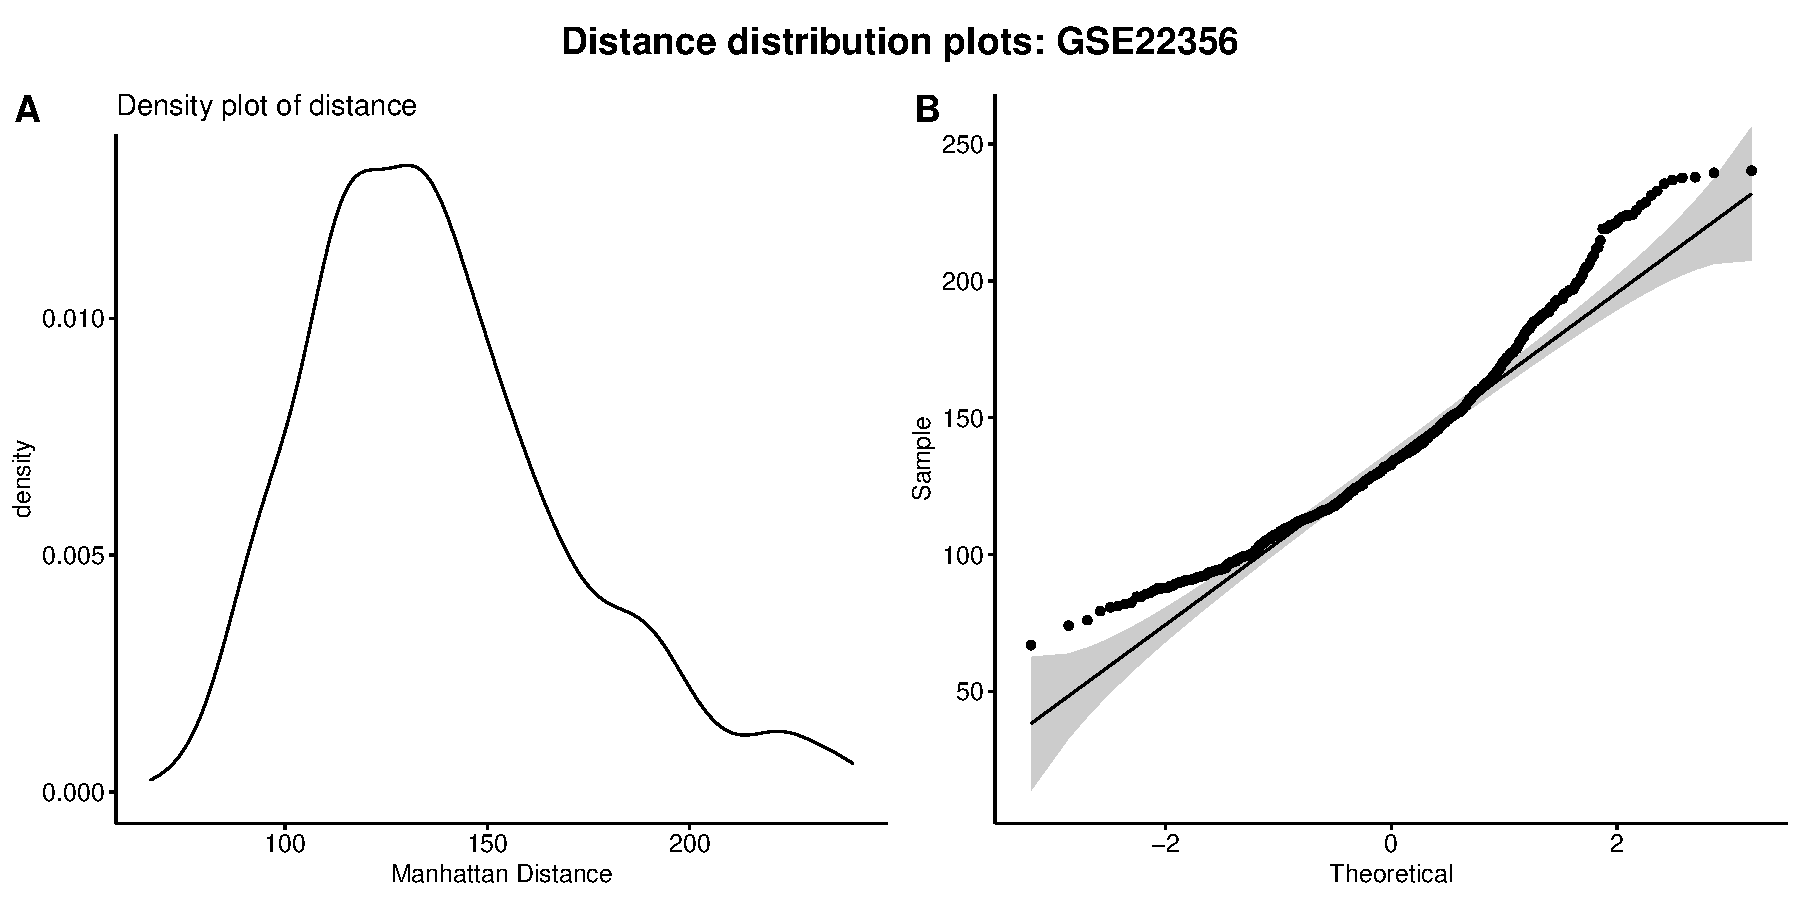
\includegraphics[width=\textwidth]{manhattan-distance_hist_GSE22356.pdf}
	\caption{Density and quantile-quantile plots for distances between samples in GSE22356. \textbf{A} Estimated density curve for distances. \textbf{B} Quantile-quantile plot between theoretical (standard normal) quantiles and sample distance quantiles.}
\end{figure}

\begin{figure}[H]
	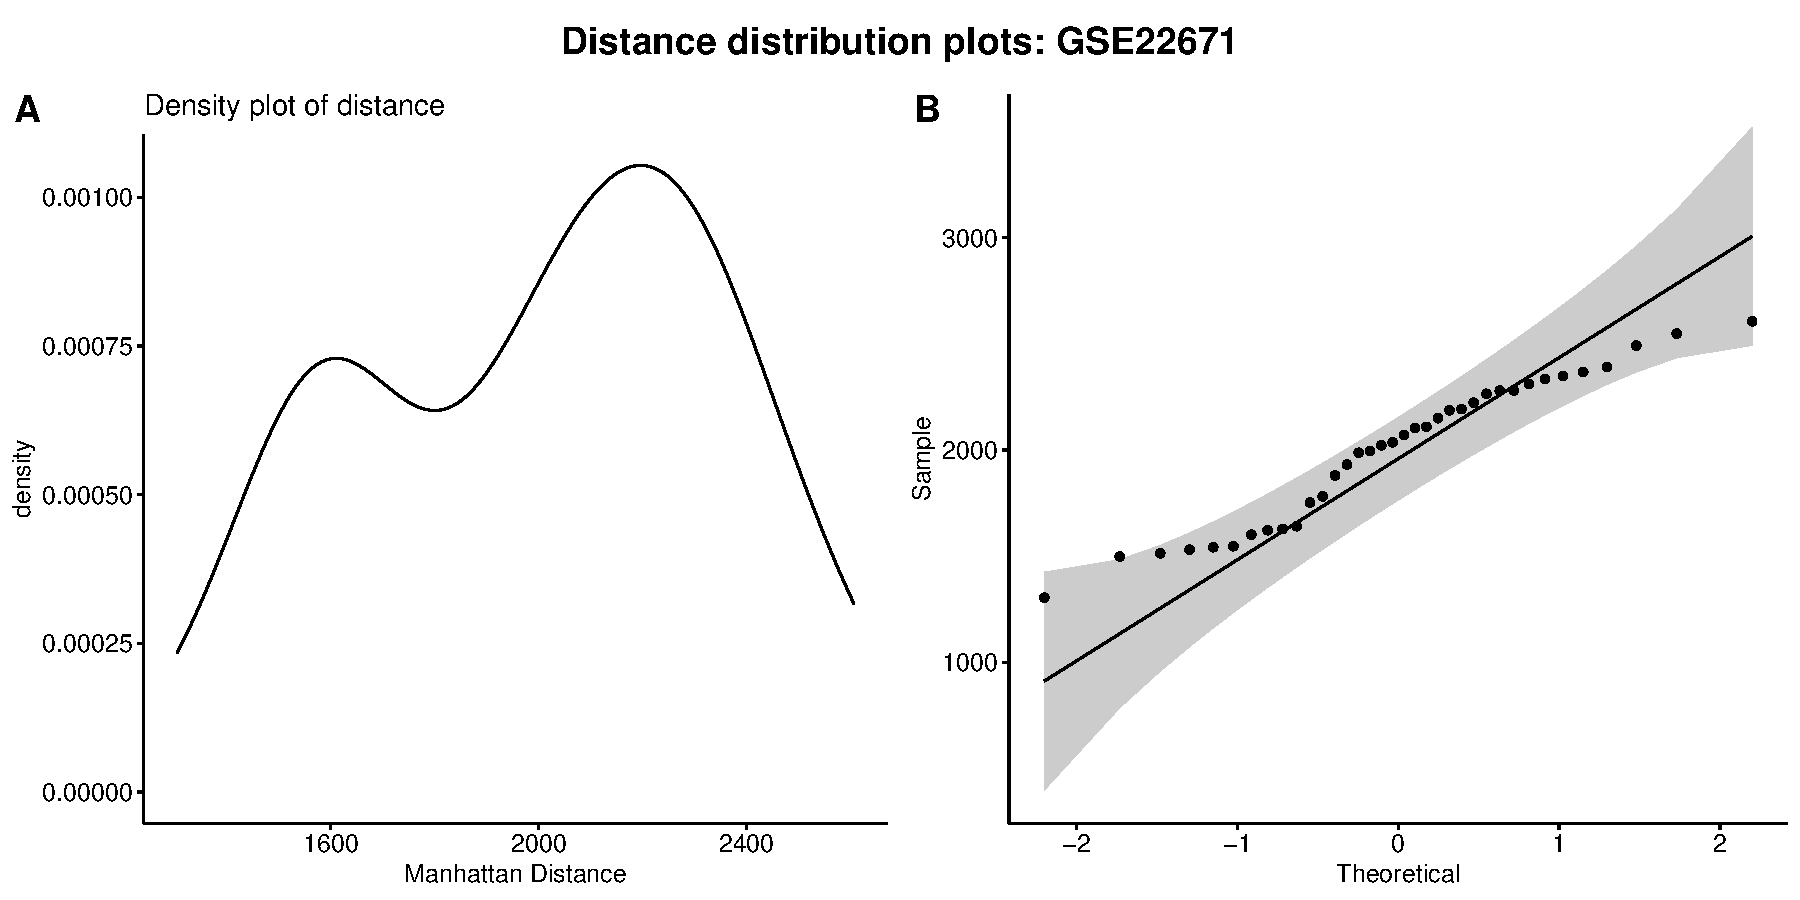
\includegraphics[width=\textwidth]{manhattan-distance_hist_GSE22671.pdf}
	\caption{Density and quantile-quantile plots for distances between samples in GSE22671. \textbf{A} Estimated density curve for distances. \textbf{B} Quantile-quantile plot between theoretical (standard normal) quantiles and sample distance quantiles.}
\end{figure}

\begin{figure}[H]
	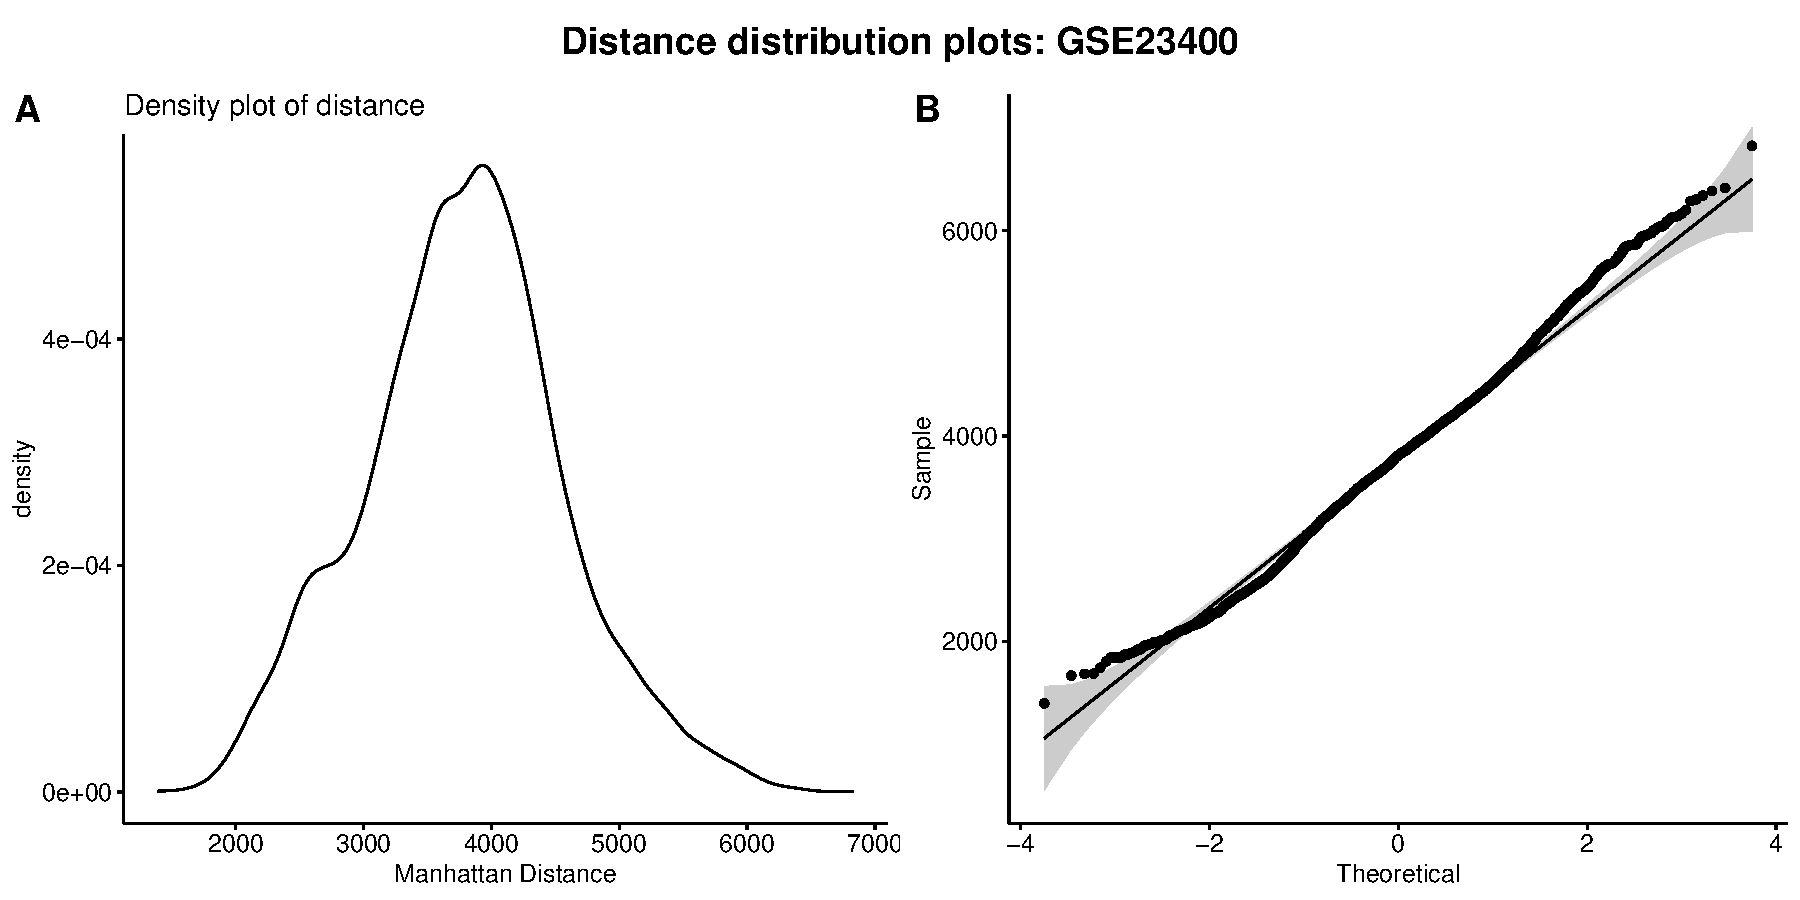
\includegraphics[width=\textwidth]{manhattan-distance_hist_GSE23400.pdf}
	\caption{Density and quantile-quantile plots for distances between samples in GSE23400. \textbf{A} Estimated density curve for distances. \textbf{B} Quantile-quantile plot between theoretical (standard normal) quantiles and sample distance quantiles.}
\end{figure}

\begin{figure}[H]
	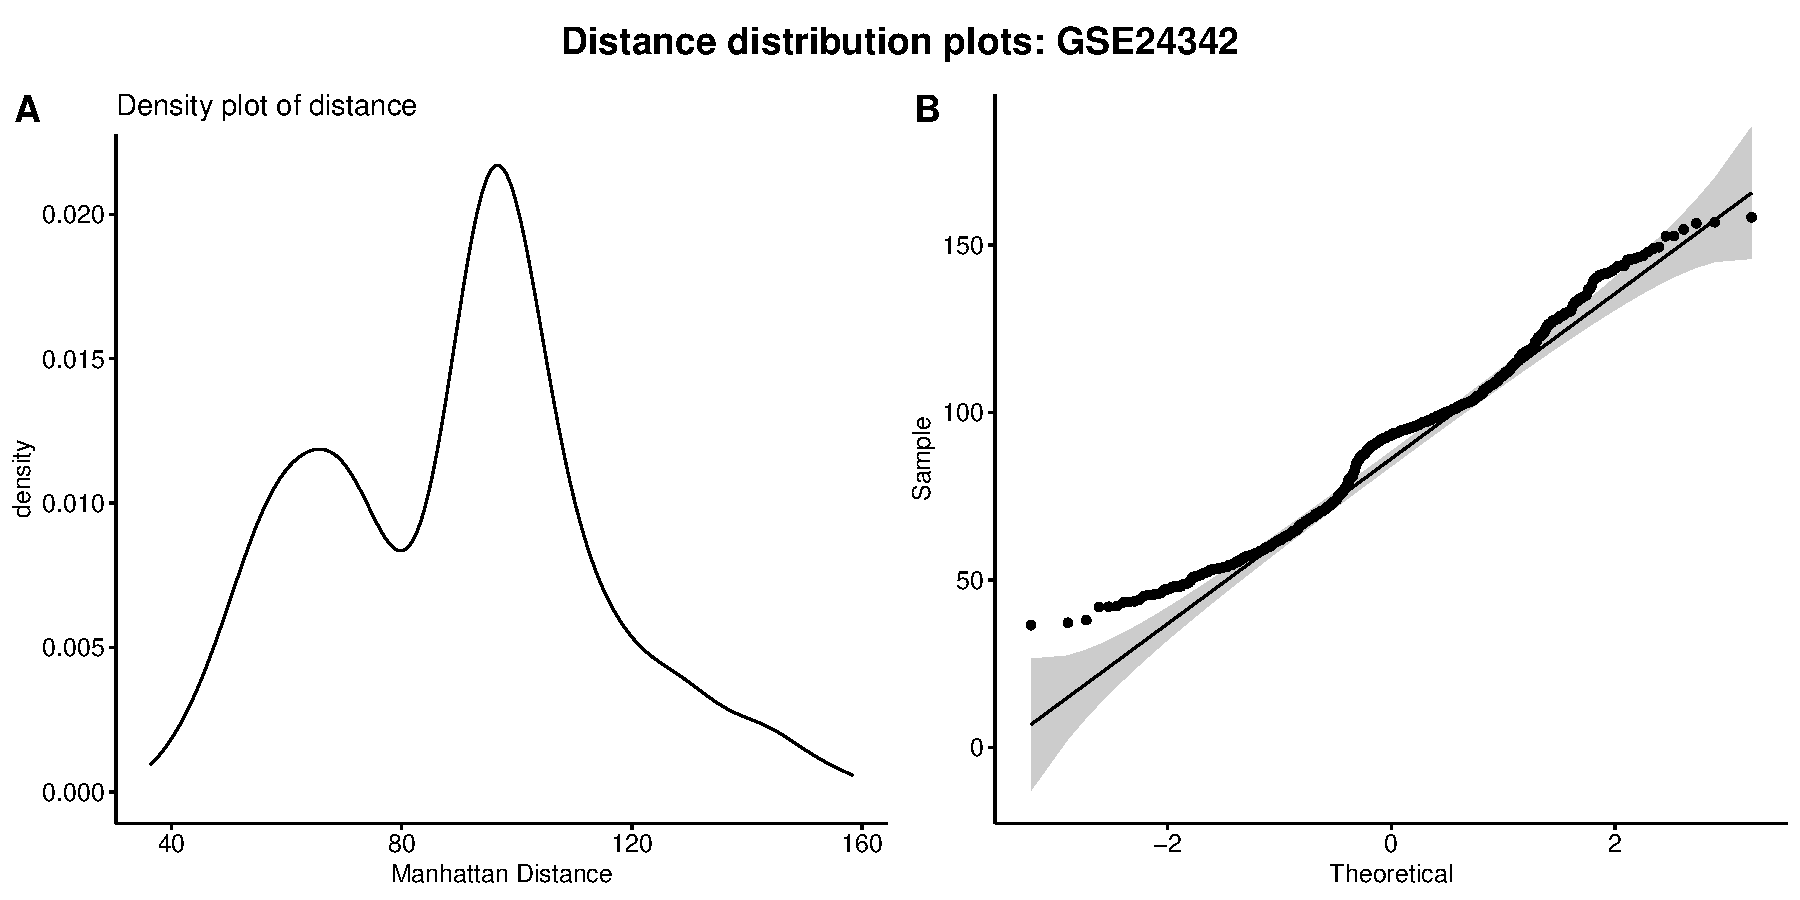
\includegraphics[width=\textwidth]{manhattan-distance_hist_GSE24342.pdf}
	\caption{Density and quantile-quantile plots for distances between samples in GSE24342. \textbf{A} Estimated density curve for distances. \textbf{B} Quantile-quantile plot between theoretical (standard normal) quantiles and sample distance quantiles.}
\end{figure}

\begin{figure}[H]
	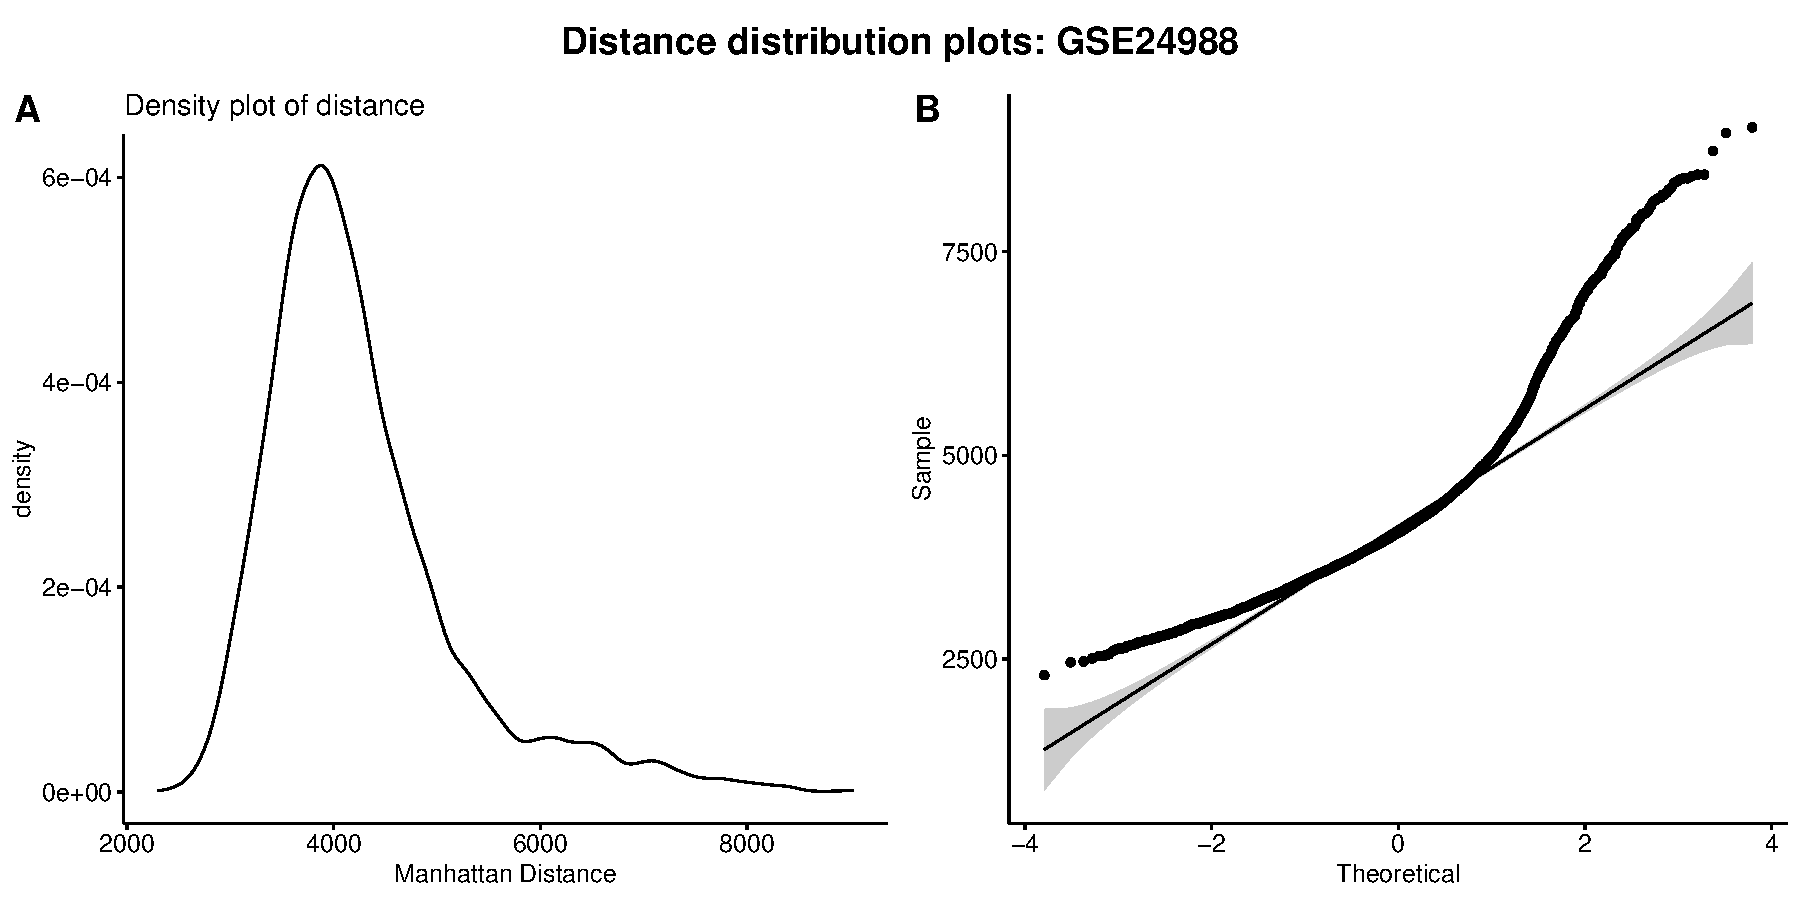
\includegraphics[width=\textwidth]{manhattan-distance_hist_GSE24988.pdf}
	\caption{Density and quantile-quantile plots for distances between samples in GSE24988. \textbf{A} Estimated density curve for distances. \textbf{B} Quantile-quantile plot between theoretical (standard normal) quantiles and sample distance quantiles.}
\end{figure}

\begin{figure}[H]
	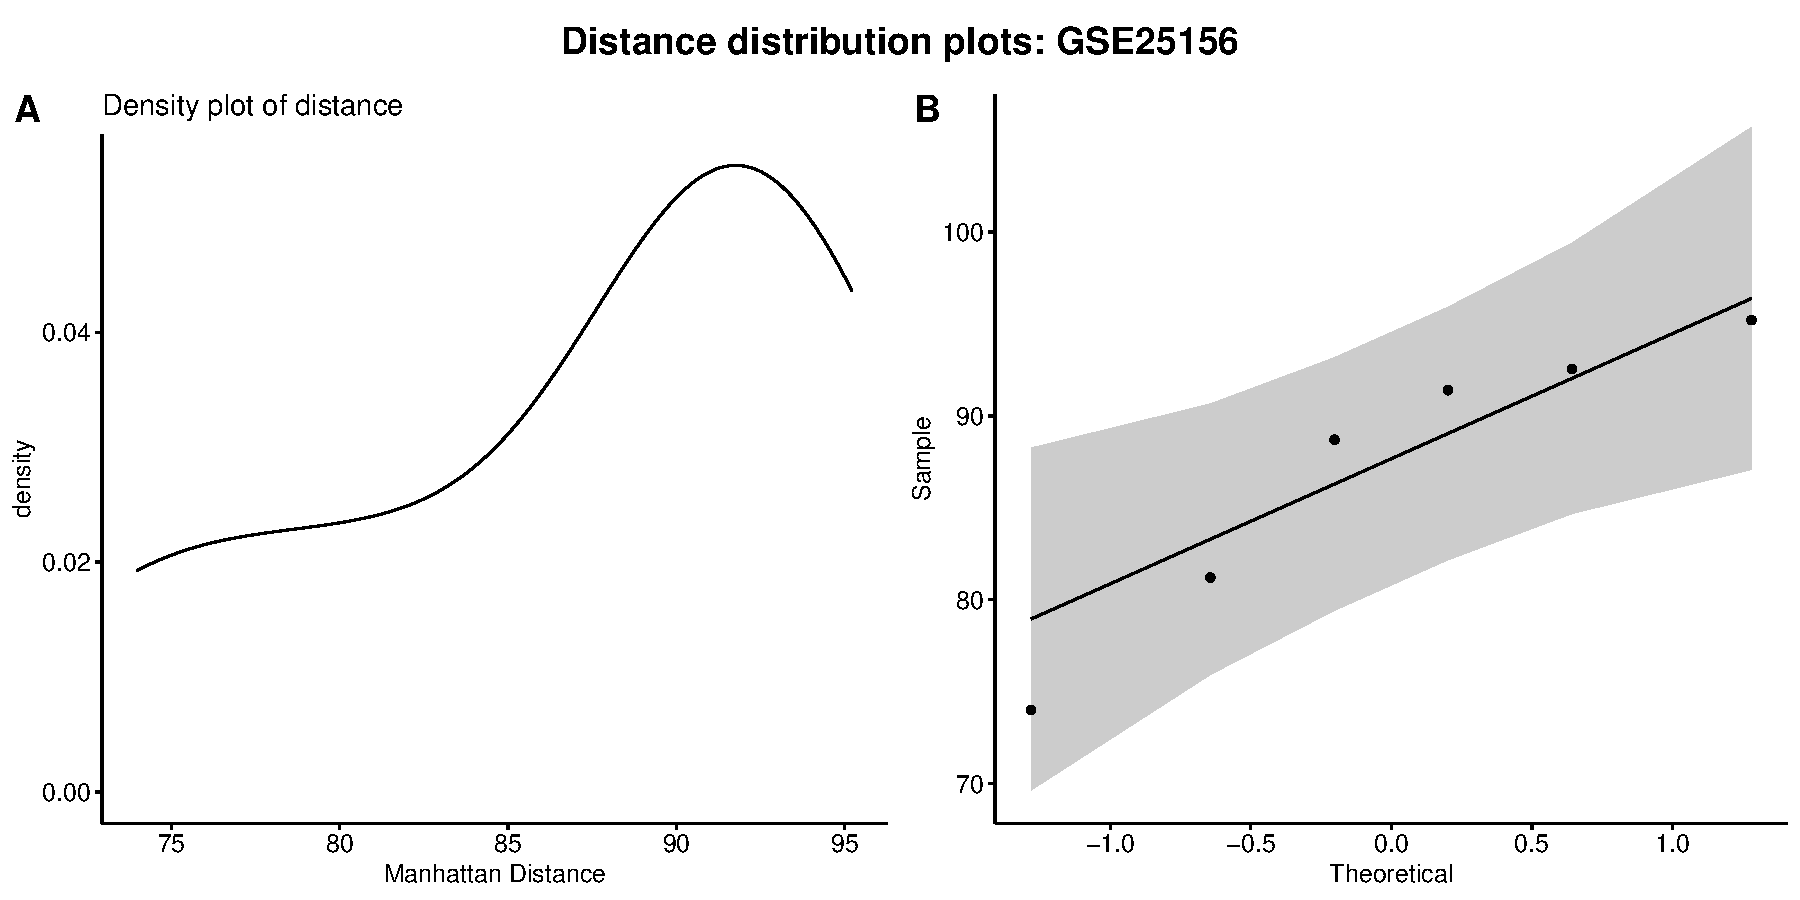
\includegraphics[width=\textwidth]{manhattan-distance_hist_GSE25156.pdf}
	\caption{Density and quantile-quantile plots for distances between samples in GSE25156. \textbf{A} Estimated density curve for distances. \textbf{B} Quantile-quantile plot between theoretical (standard normal) quantiles and sample distance quantiles.}
\end{figure}

\begin{figure}[H]
	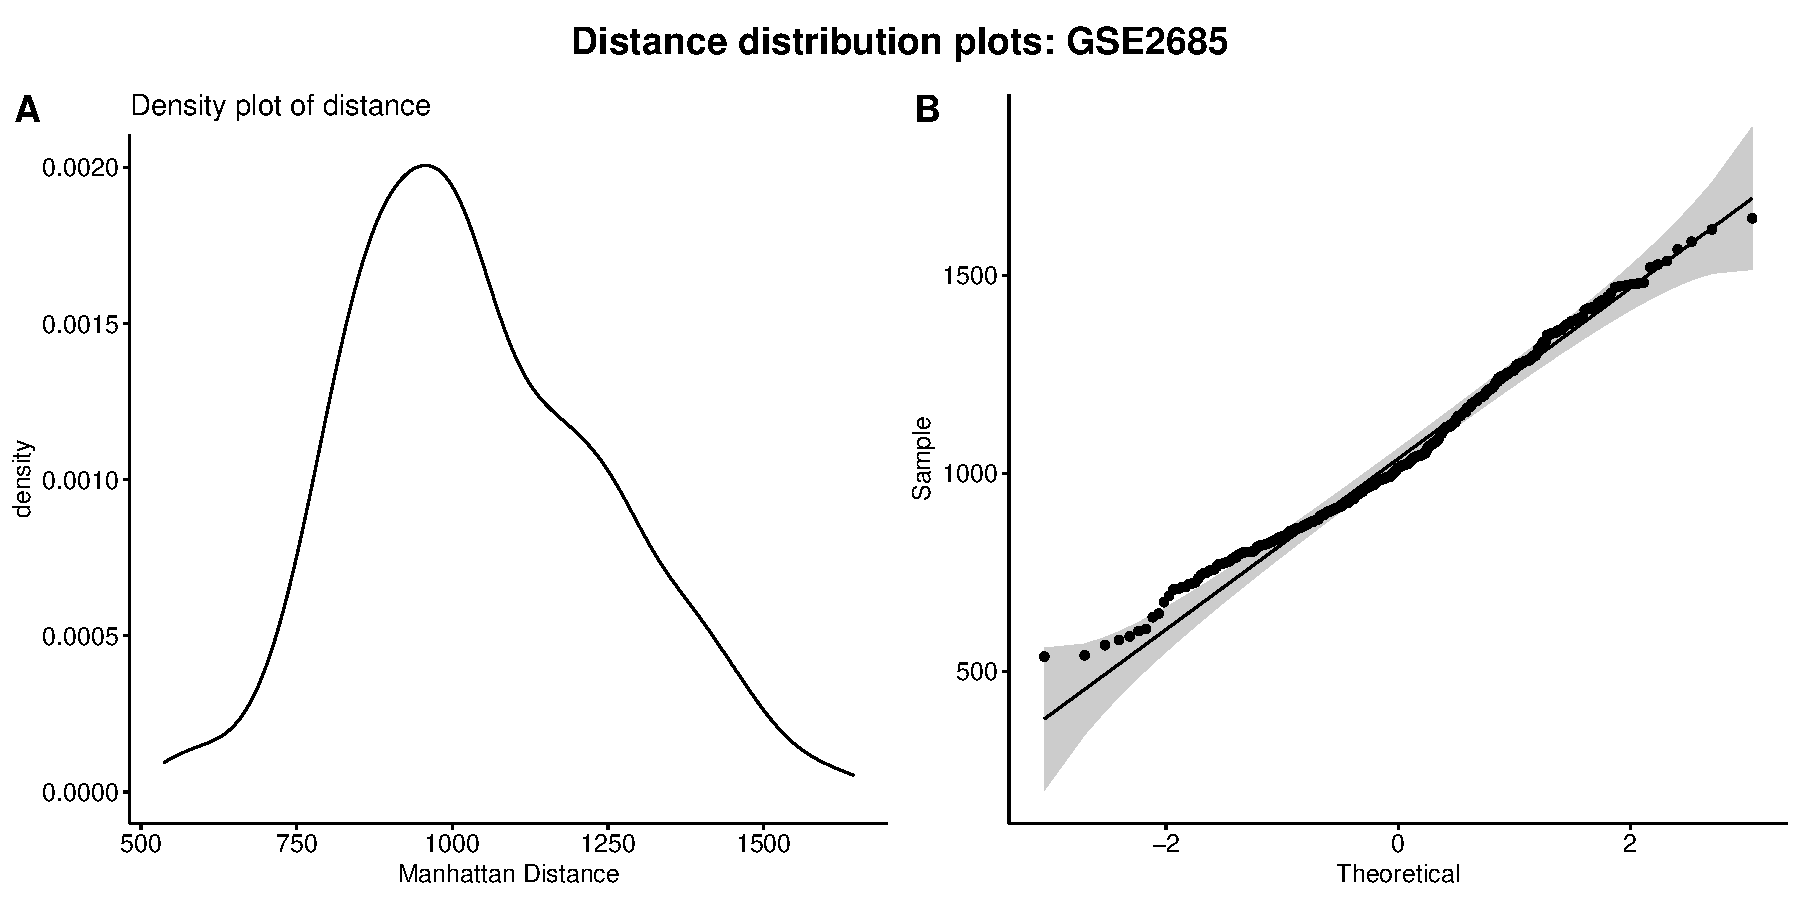
\includegraphics[width=\textwidth]{manhattan-distance_hist_GSE2685.pdf}
	\caption{Density and quantile-quantile plots for distances between samples in GSE2685. \textbf{A} Estimated density curve for distances. \textbf{B} Quantile-quantile plot between theoretical (standard normal) quantiles and sample distance quantiles.}
\end{figure}

\begin{figure}[H]
	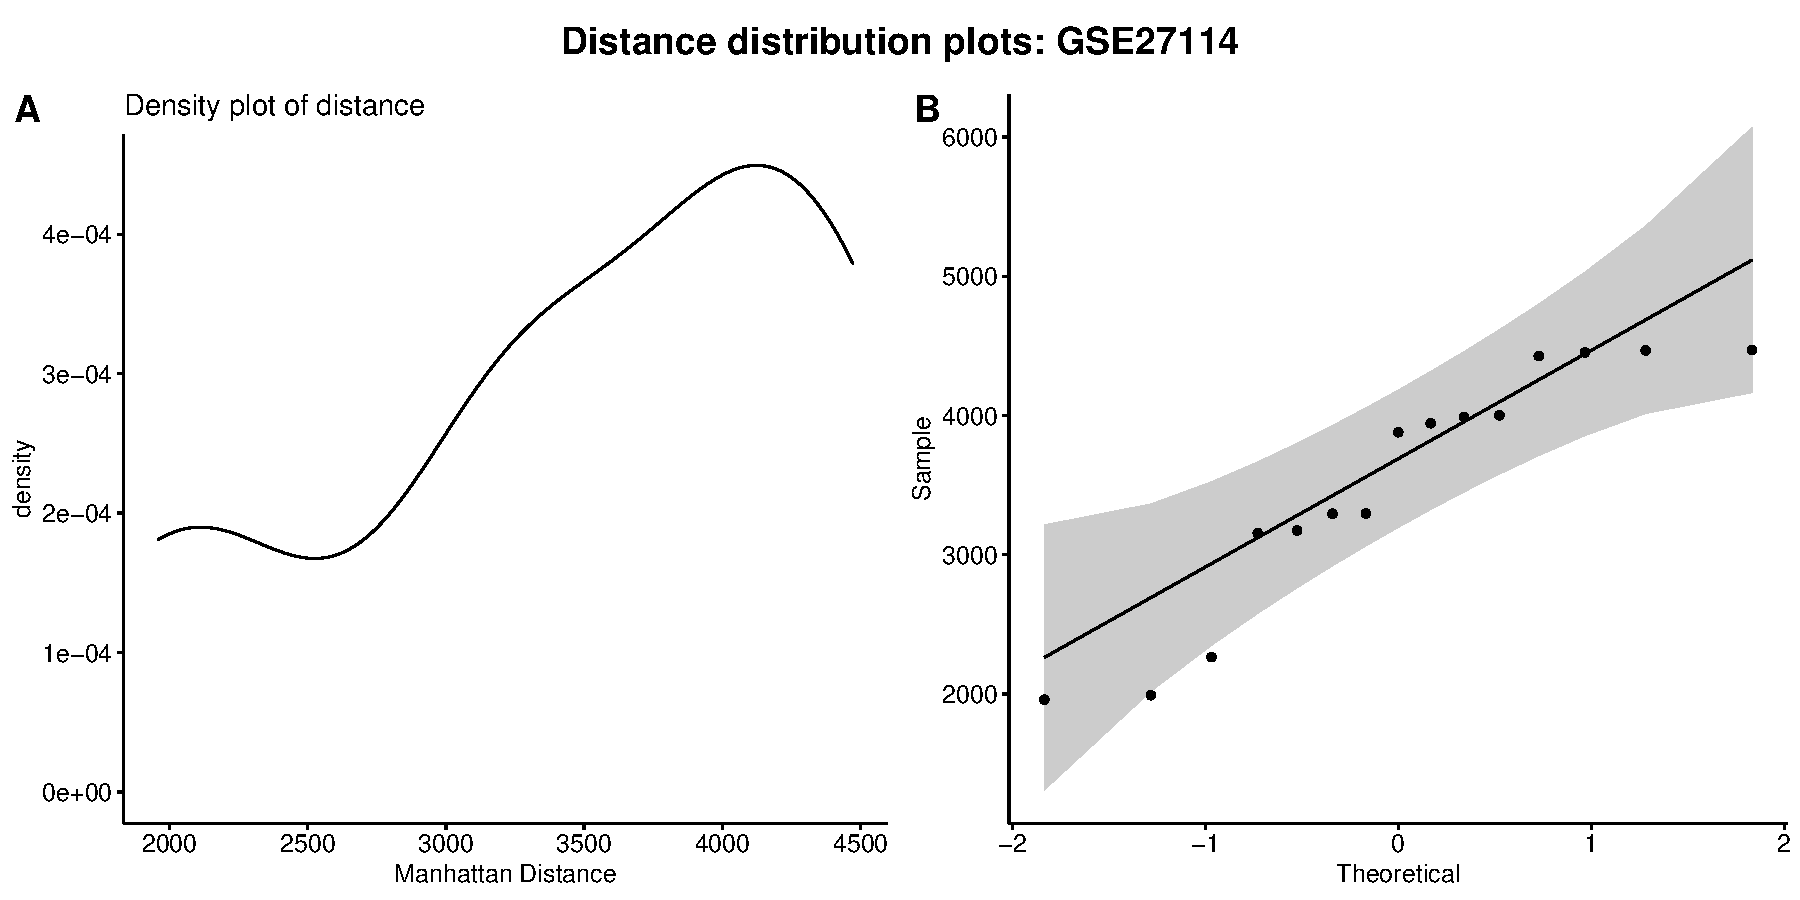
\includegraphics[width=\textwidth]{manhattan-distance_hist_GSE27114.pdf}
	\caption{Density and quantile-quantile plots for distances between samples in GSE27114. \textbf{A} Estimated density curve for distances. \textbf{B} Quantile-quantile plot between theoretical (standard normal) quantiles and sample distance quantiles.}
\end{figure}

\begin{figure}[H]
	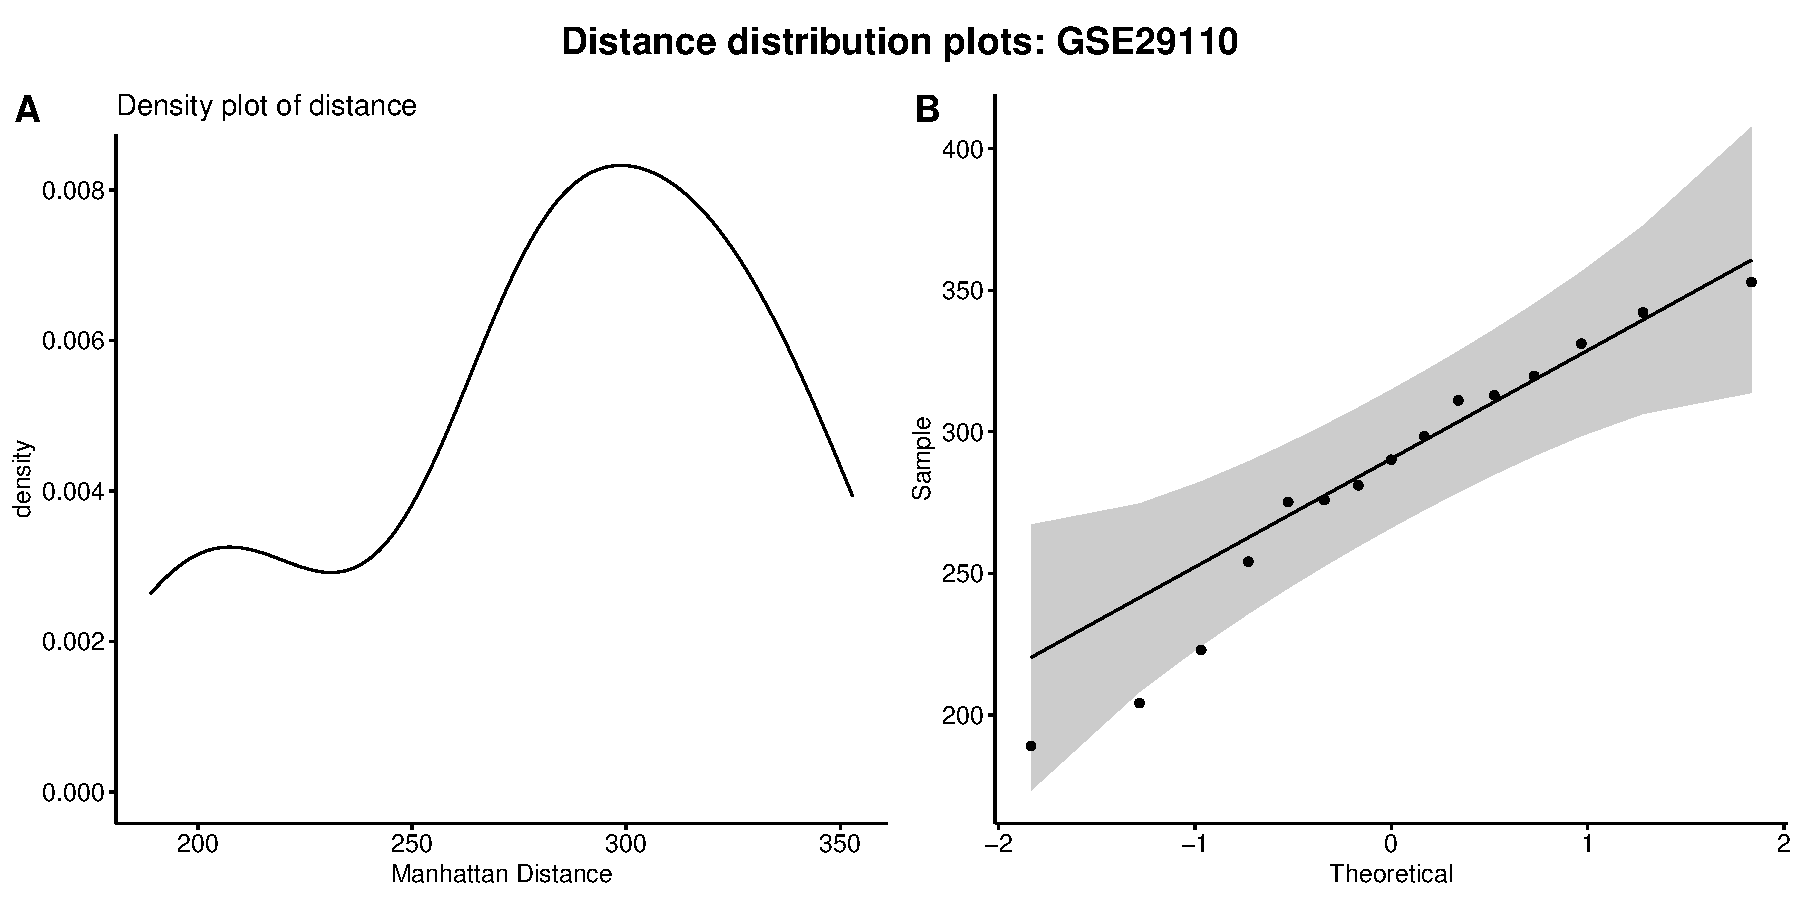
\includegraphics[width=\textwidth]{manhattan-distance_hist_GSE29110.pdf}
	\caption{Density and quantile-quantile plots for distances between samples in GSE29110. \textbf{A} Estimated density curve for distances. \textbf{B} Quantile-quantile plot between theoretical (standard normal) quantiles and sample distance quantiles.}
\end{figure}

\begin{figure}[H]
	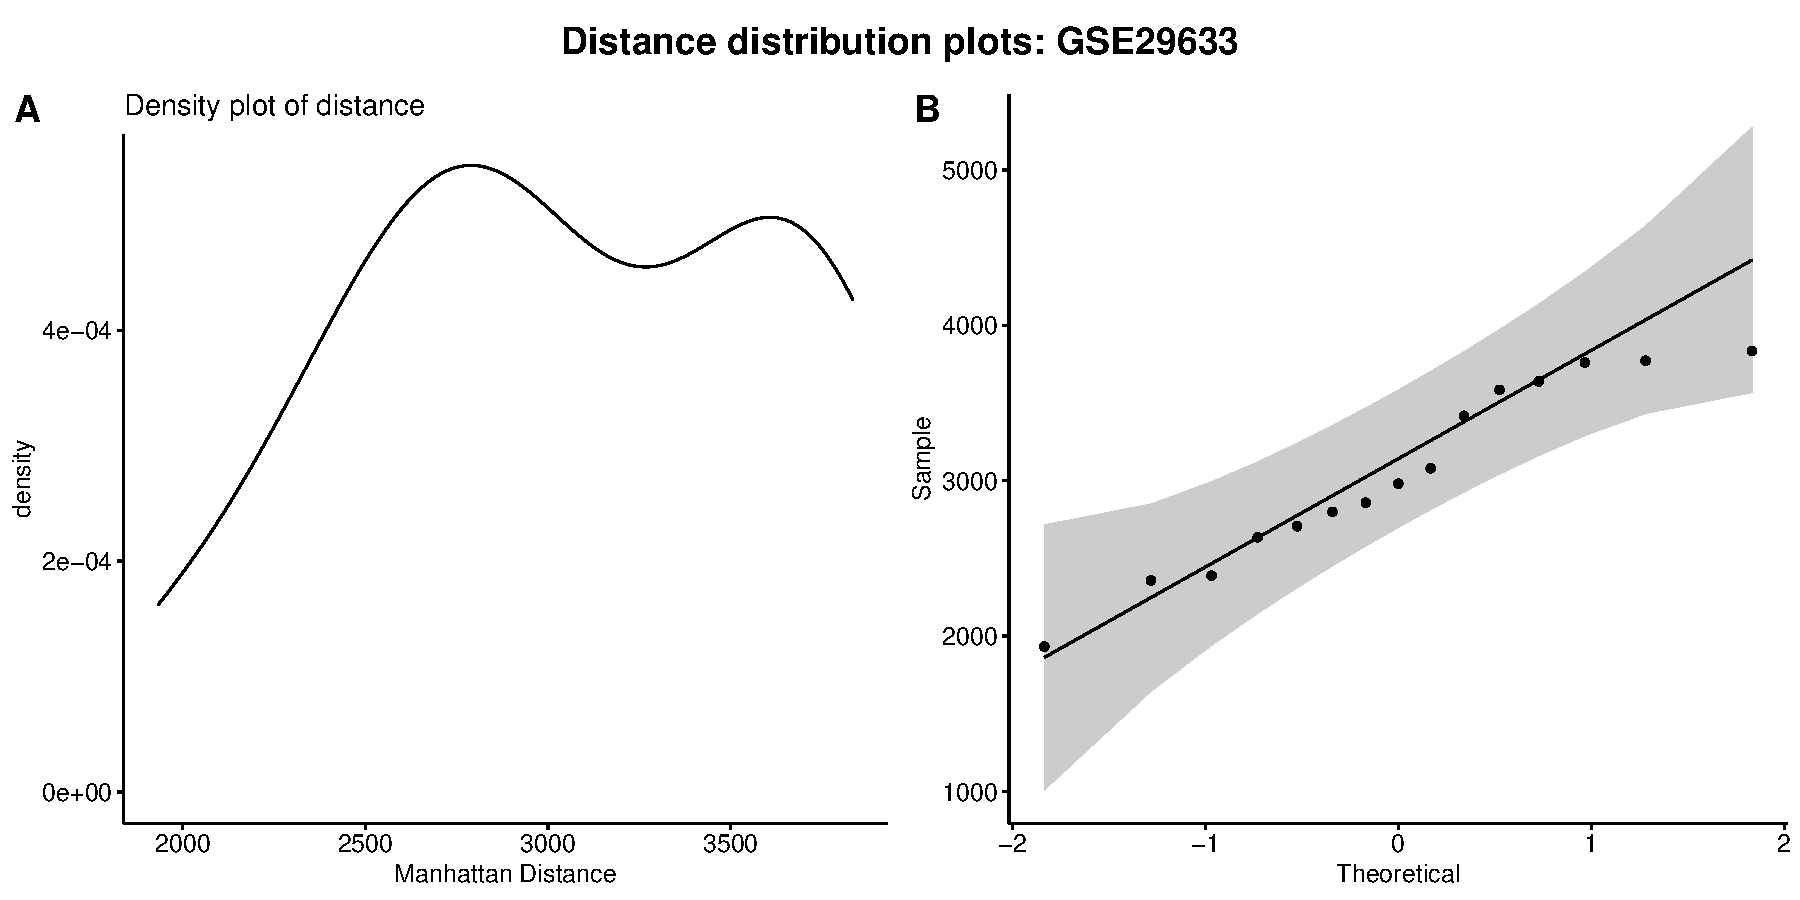
\includegraphics[width=\textwidth]{manhattan-distance_hist_GSE29633.pdf}
	\caption{Density and quantile-quantile plots for distances between samples in GSE29633. \textbf{A} Estimated density curve for distances. \textbf{B} Quantile-quantile plot between theoretical (standard normal) quantiles and sample distance quantiles.}
\end{figure}

\begin{figure}[H]
	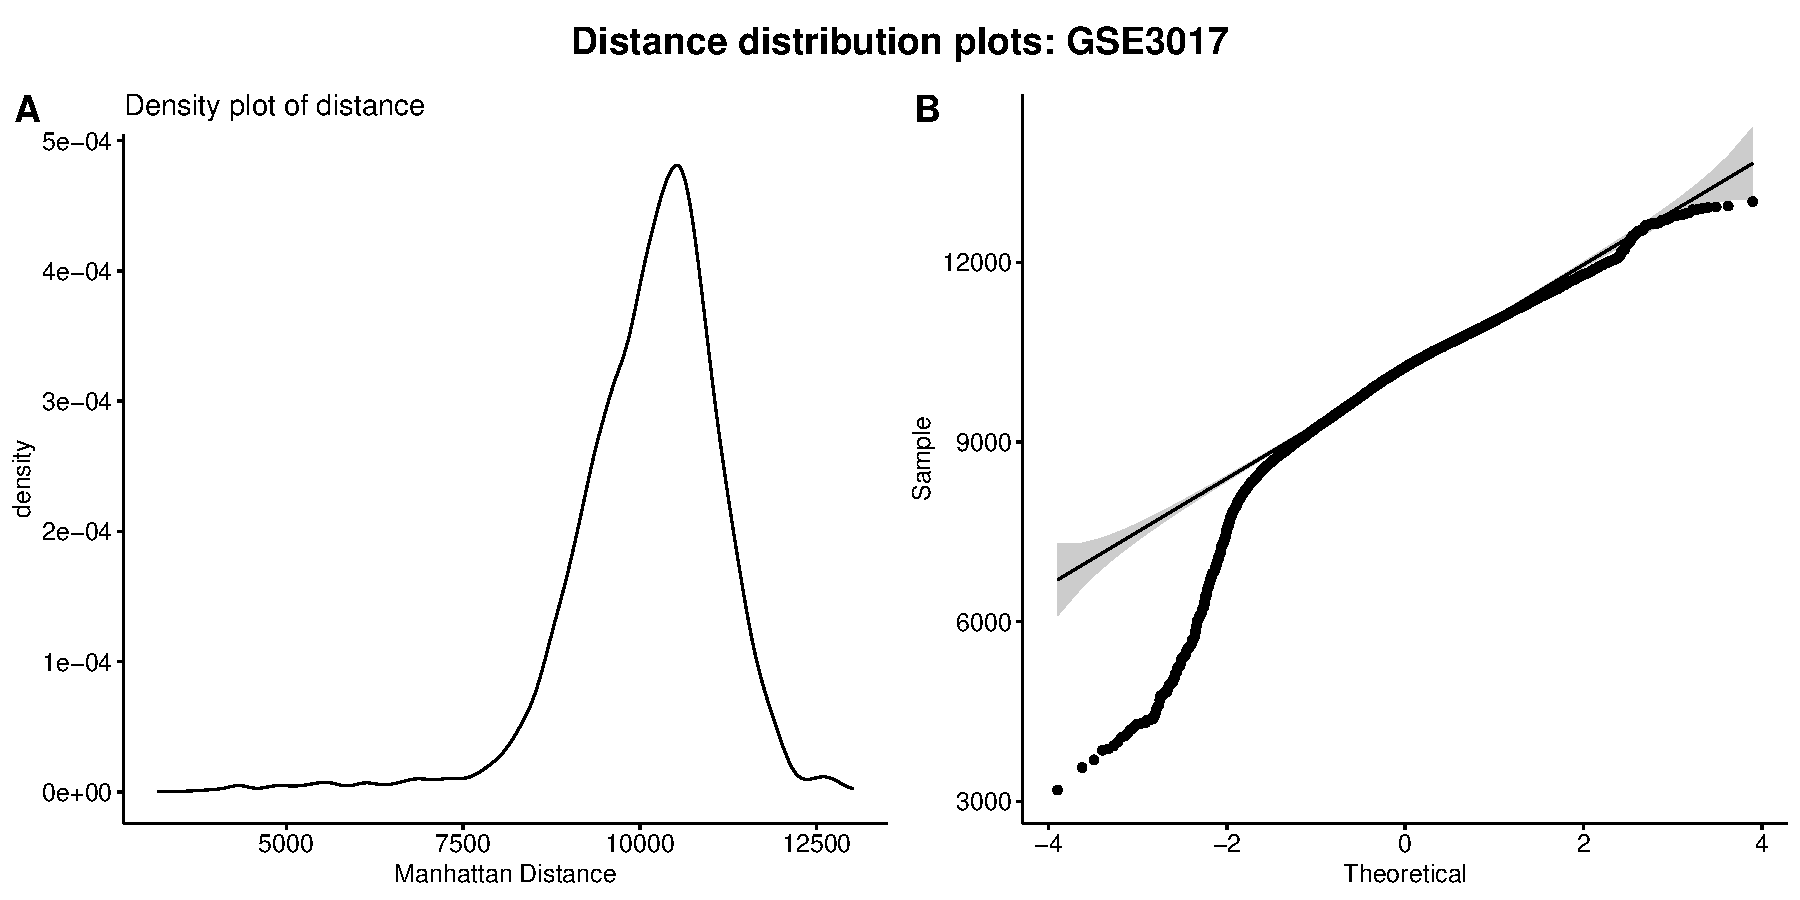
\includegraphics[width=\textwidth]{manhattan-distance_hist_GSE3017.pdf}
	\caption{Density and quantile-quantile plots for distances between samples in GSE3017. \textbf{A} Estimated density curve for distances. \textbf{B} Quantile-quantile plot between theoretical (standard normal) quantiles and sample distance quantiles.}
\end{figure}

\begin{figure}[H]
	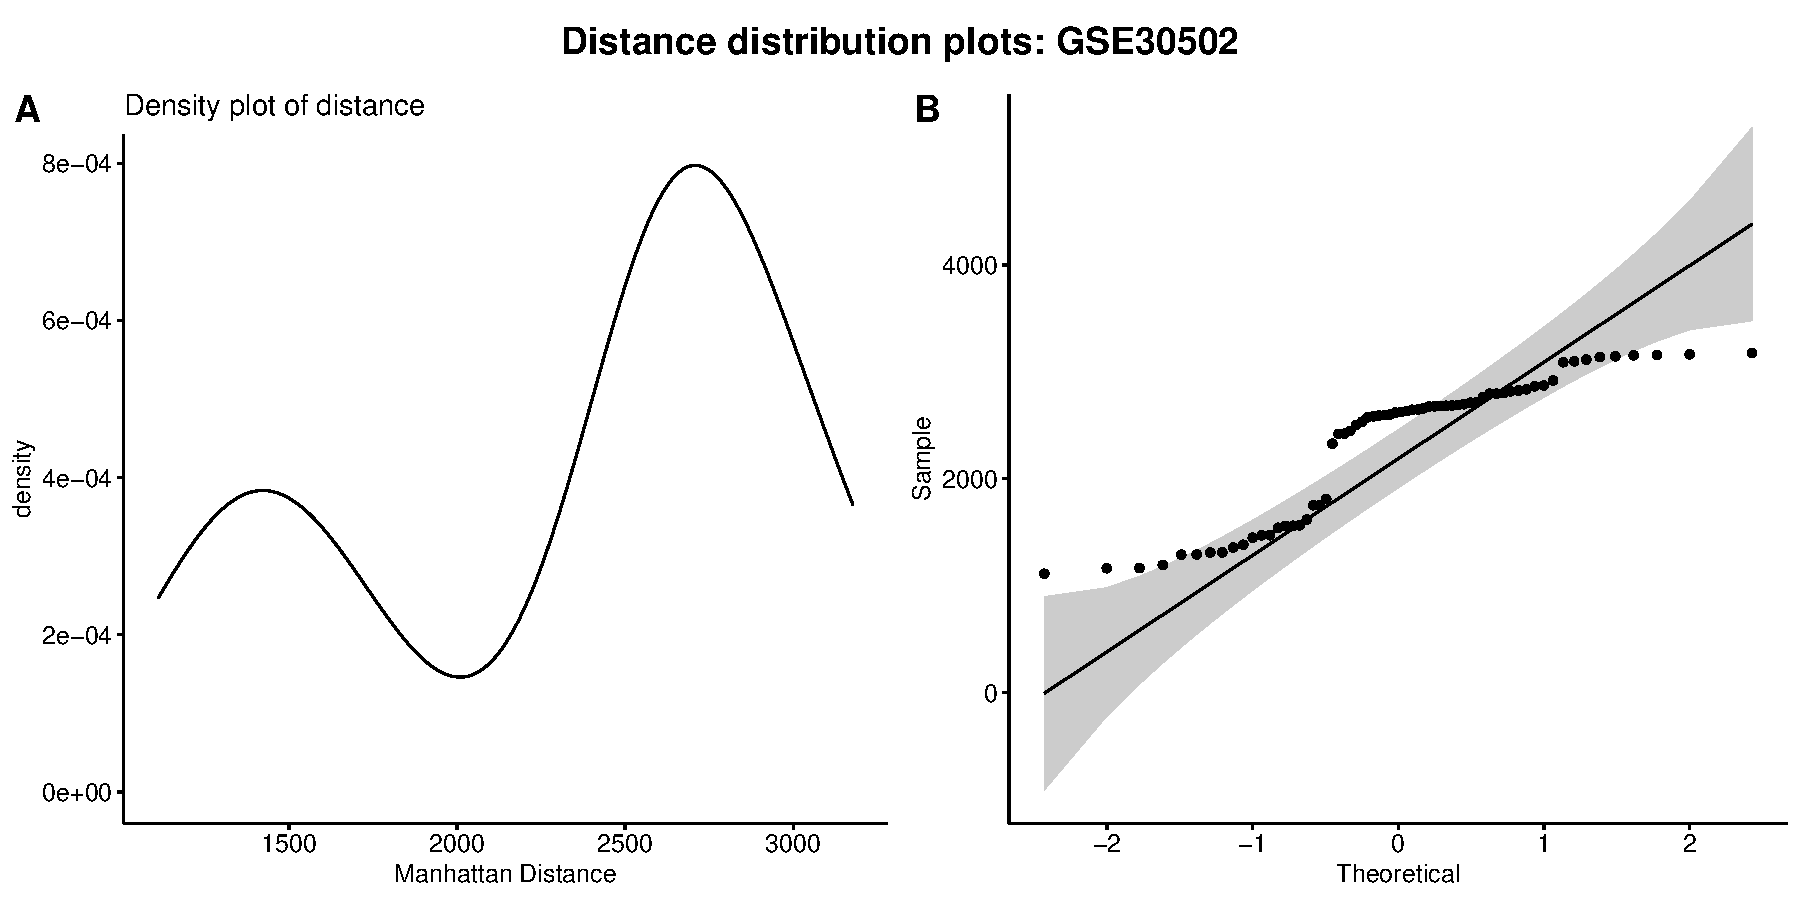
\includegraphics[width=\textwidth]{manhattan-distance_hist_GSE30502.pdf}
	\caption{Density and quantile-quantile plots for distances between samples in GSE30502. \textbf{A} Estimated density curve for distances. \textbf{B} Quantile-quantile plot between theoretical (standard normal) quantiles and sample distance quantiles.}
\end{figure}

\begin{figure}[H]
	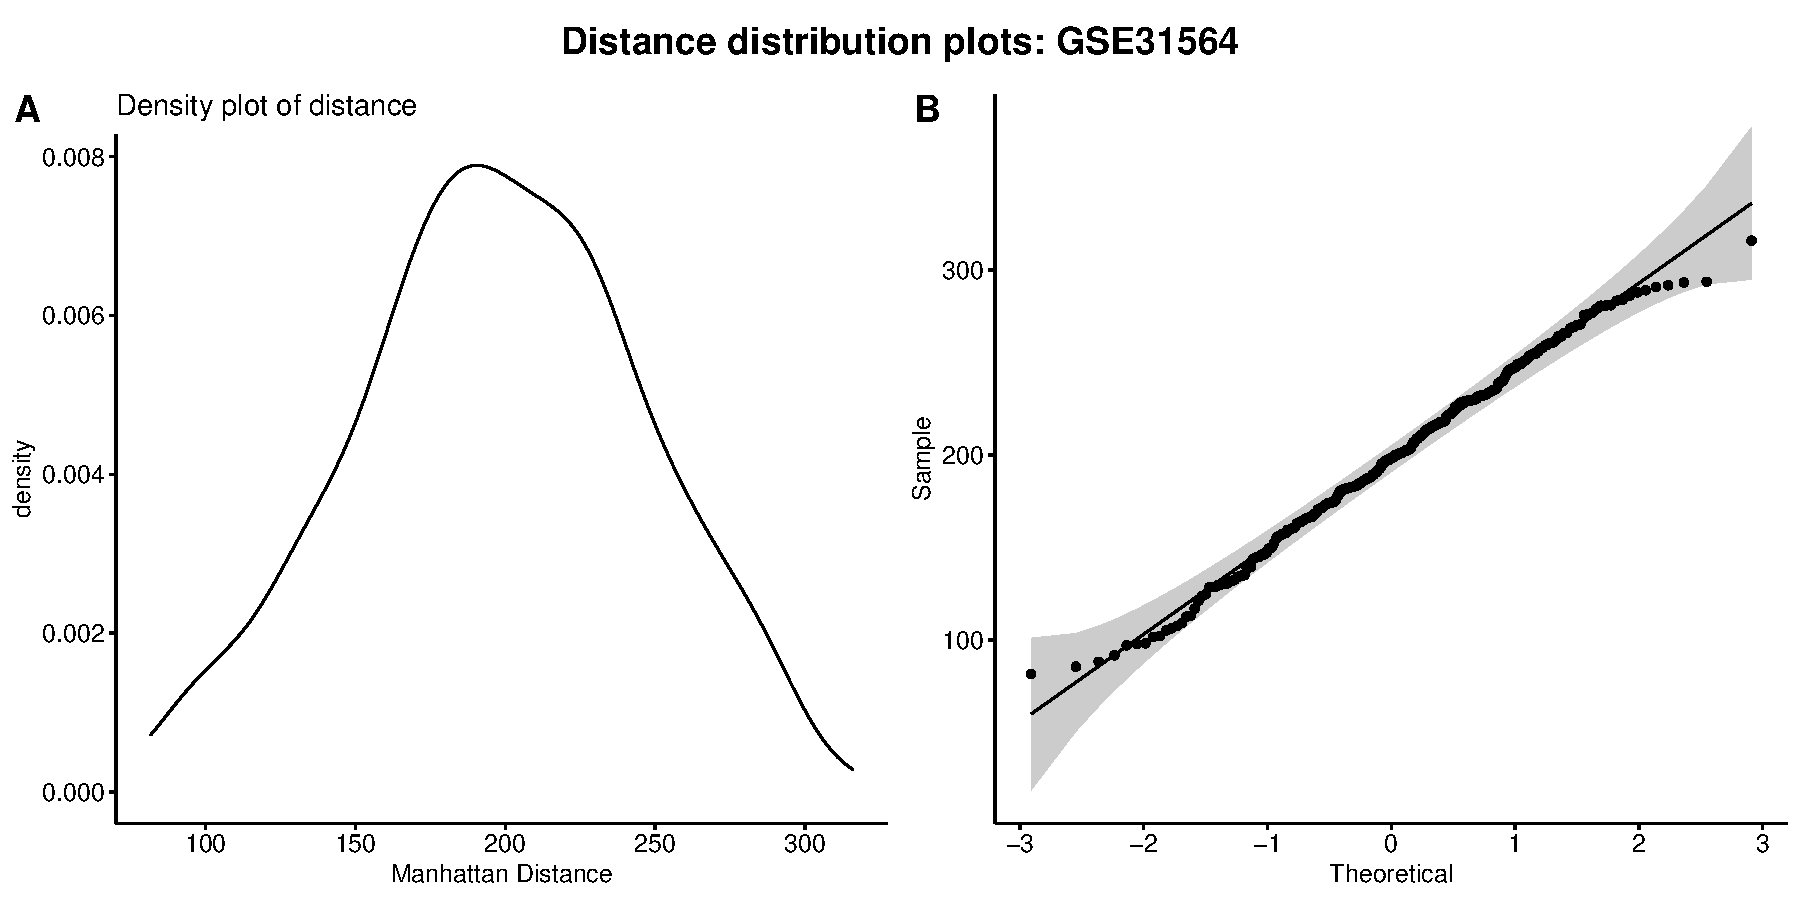
\includegraphics[width=\textwidth]{manhattan-distance_hist_GSE31564.pdf}
	\caption{Density and quantile-quantile plots for distances between samples in GSE31564. \textbf{A} Estimated density curve for distances. \textbf{B} Quantile-quantile plot between theoretical (standard normal) quantiles and sample distance quantiles.}
\end{figure}

\begin{figure}[H]
	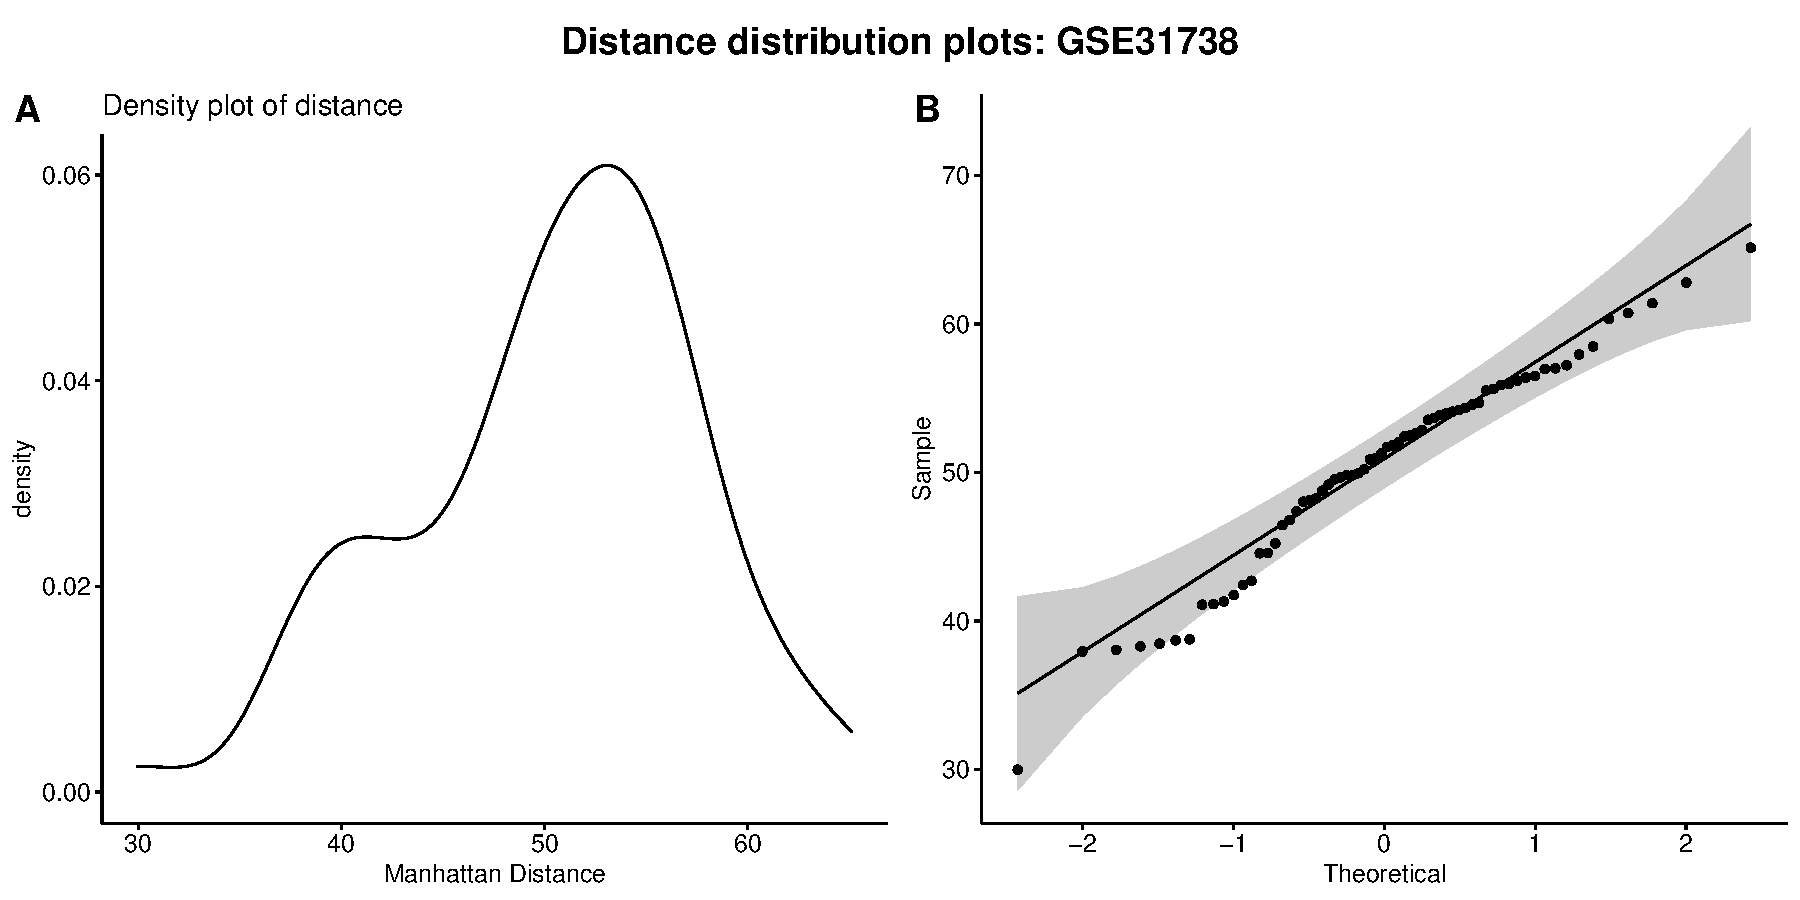
\includegraphics[width=\textwidth]{manhattan-distance_hist_GSE31738.pdf}
	\caption{Density and quantile-quantile plots for distances between samples in GSE31738. \textbf{A} Estimated density curve for distances. \textbf{B} Quantile-quantile plot between theoretical (standard normal) quantiles and sample distance quantiles.}
\end{figure}

\begin{figure}[H]
	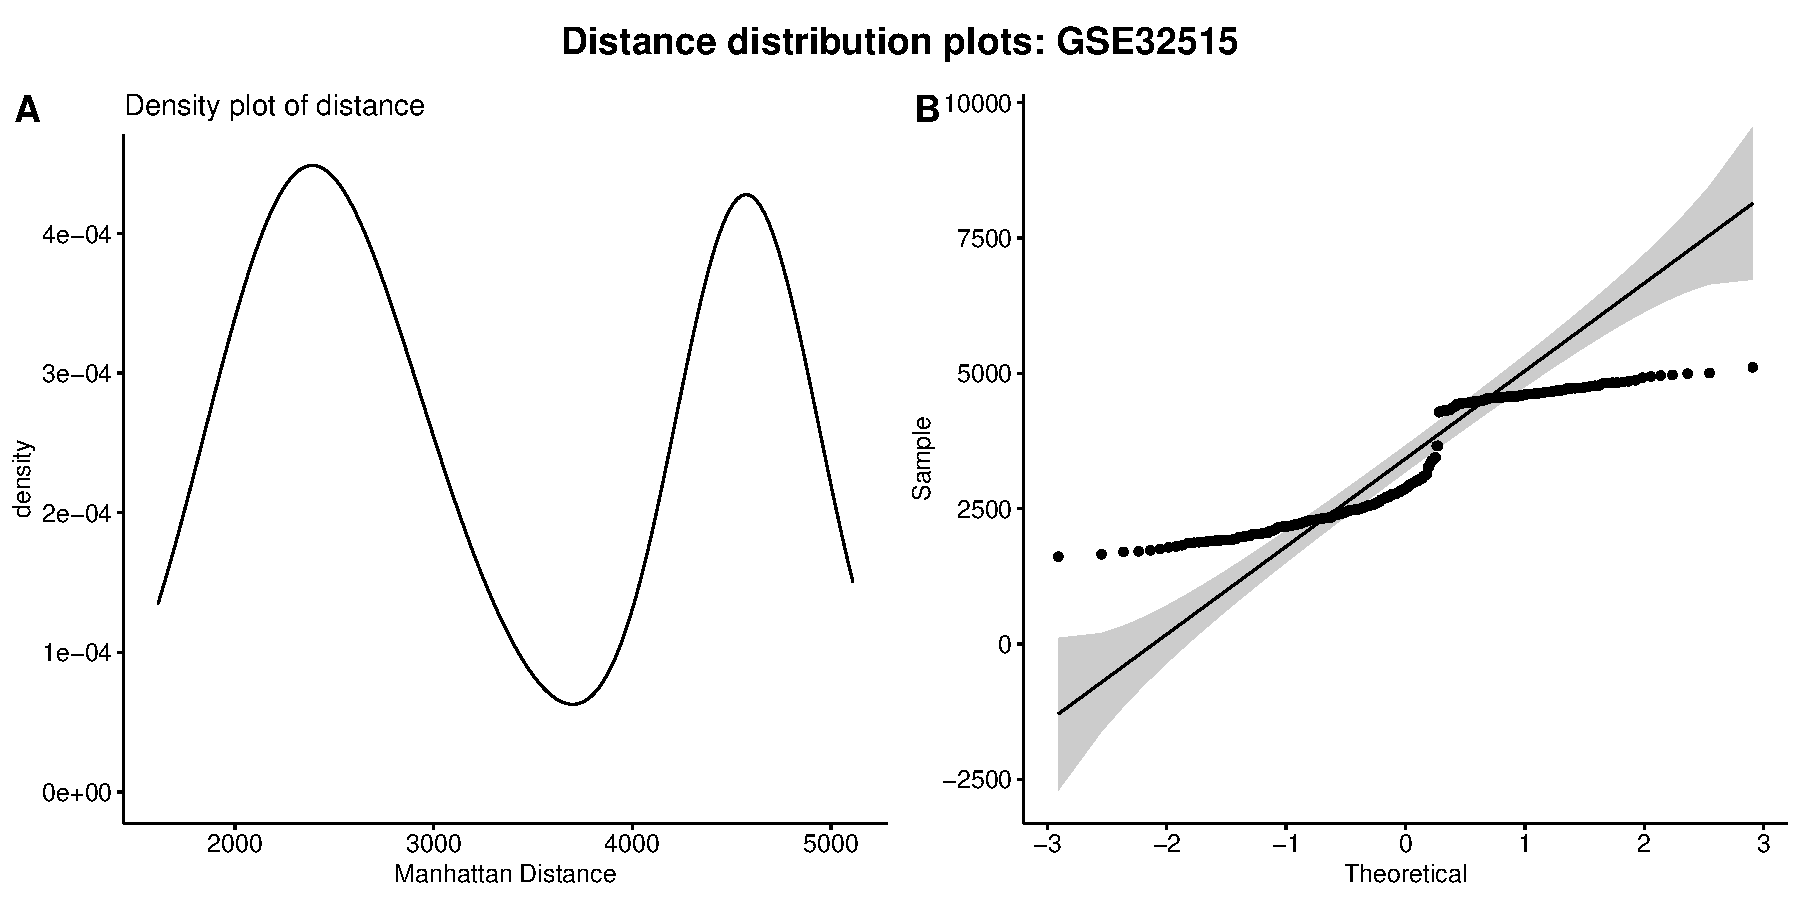
\includegraphics[width=\textwidth]{manhattan-distance_hist_GSE32515.pdf}
	\caption{Density and quantile-quantile plots for distances between samples in GSE32515. \textbf{A} Estimated density curve for distances. \textbf{B} Quantile-quantile plot between theoretical (standard normal) quantiles and sample distance quantiles.}
\end{figure}

\begin{figure}[H]
	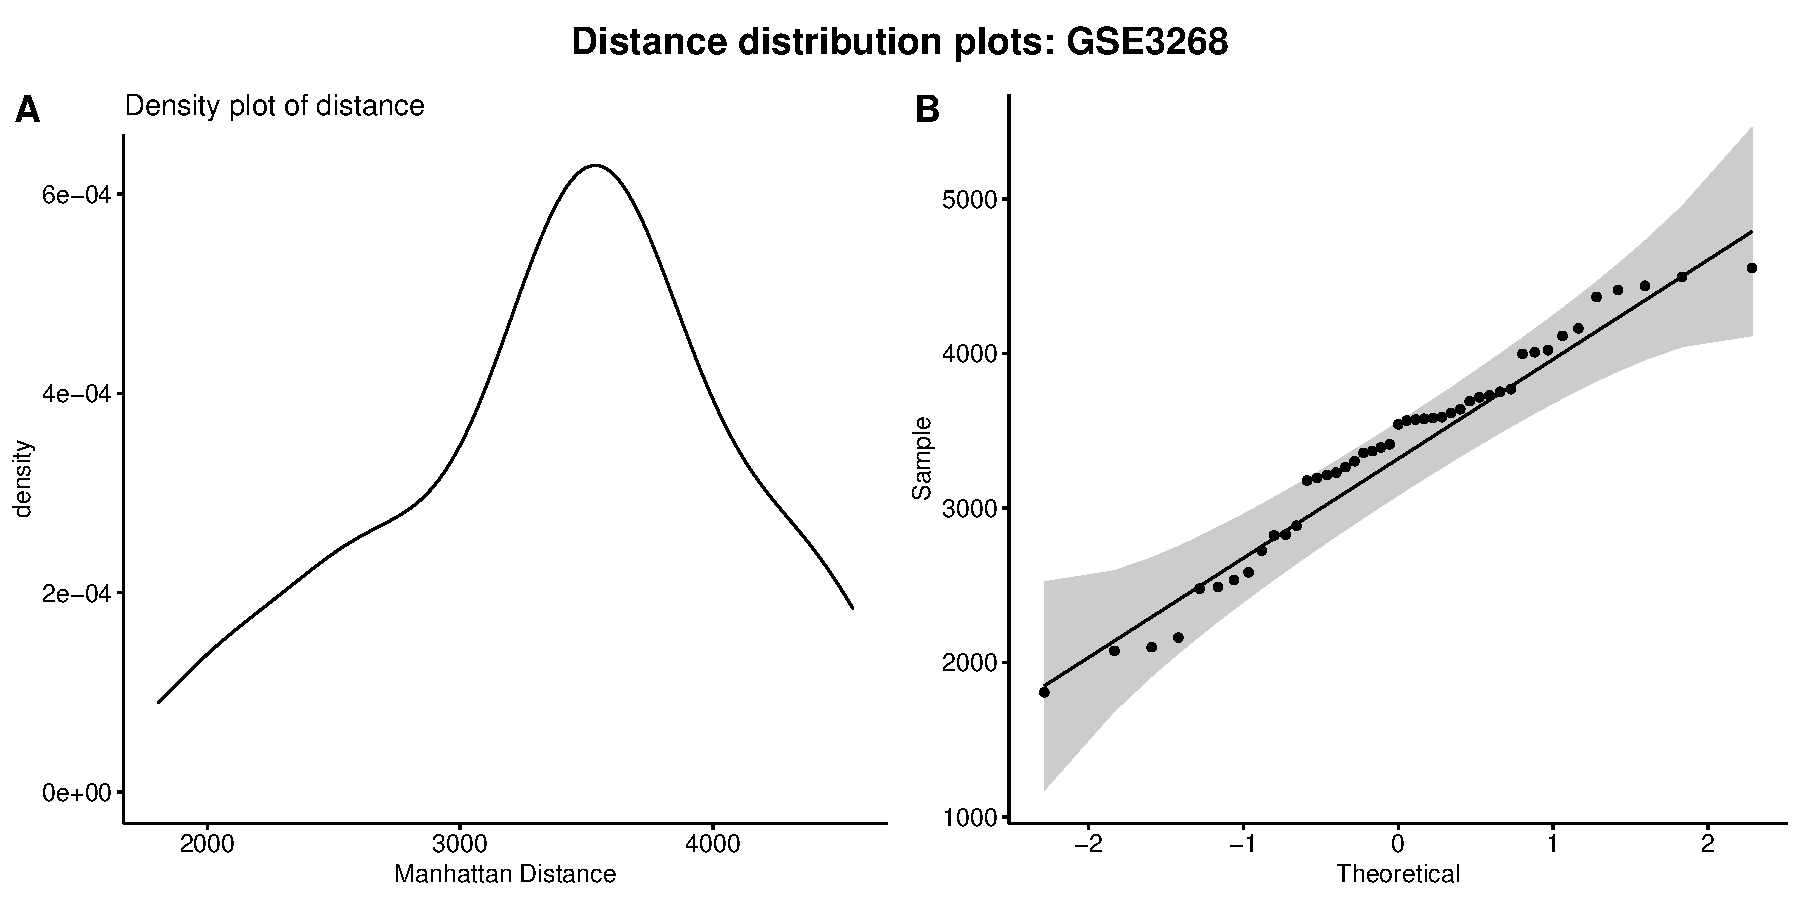
\includegraphics[width=\textwidth]{manhattan-distance_hist_GSE3268.pdf}
	\caption{Density and quantile-quantile plots for distances between samples in GSE3268. \textbf{A} Estimated density curve for distances. \textbf{B} Quantile-quantile plot between theoretical (standard normal) quantiles and sample distance quantiles.}
\end{figure}

\begin{figure}[H]
	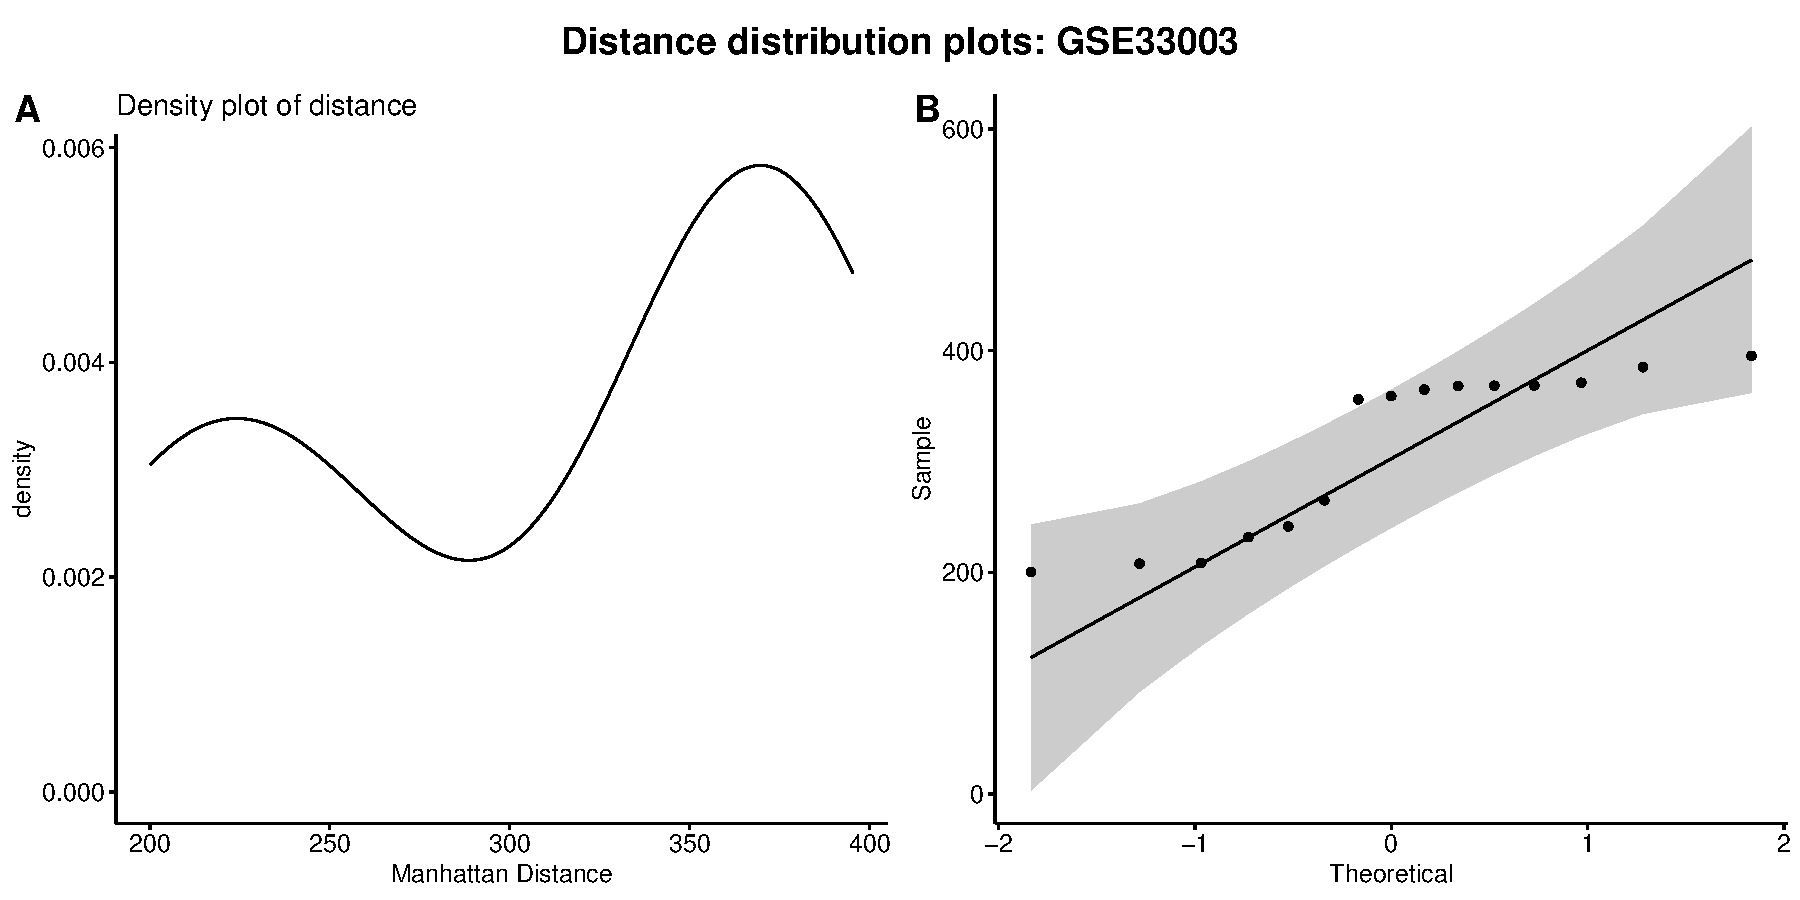
\includegraphics[width=\textwidth]{manhattan-distance_hist_GSE33003.pdf}
	\caption{Density and quantile-quantile plots for distances between samples in GSE33003. \textbf{A} Estimated density curve for distances. \textbf{B} Quantile-quantile plot between theoretical (standard normal) quantiles and sample distance quantiles.}
\end{figure}

\begin{figure}[H]
	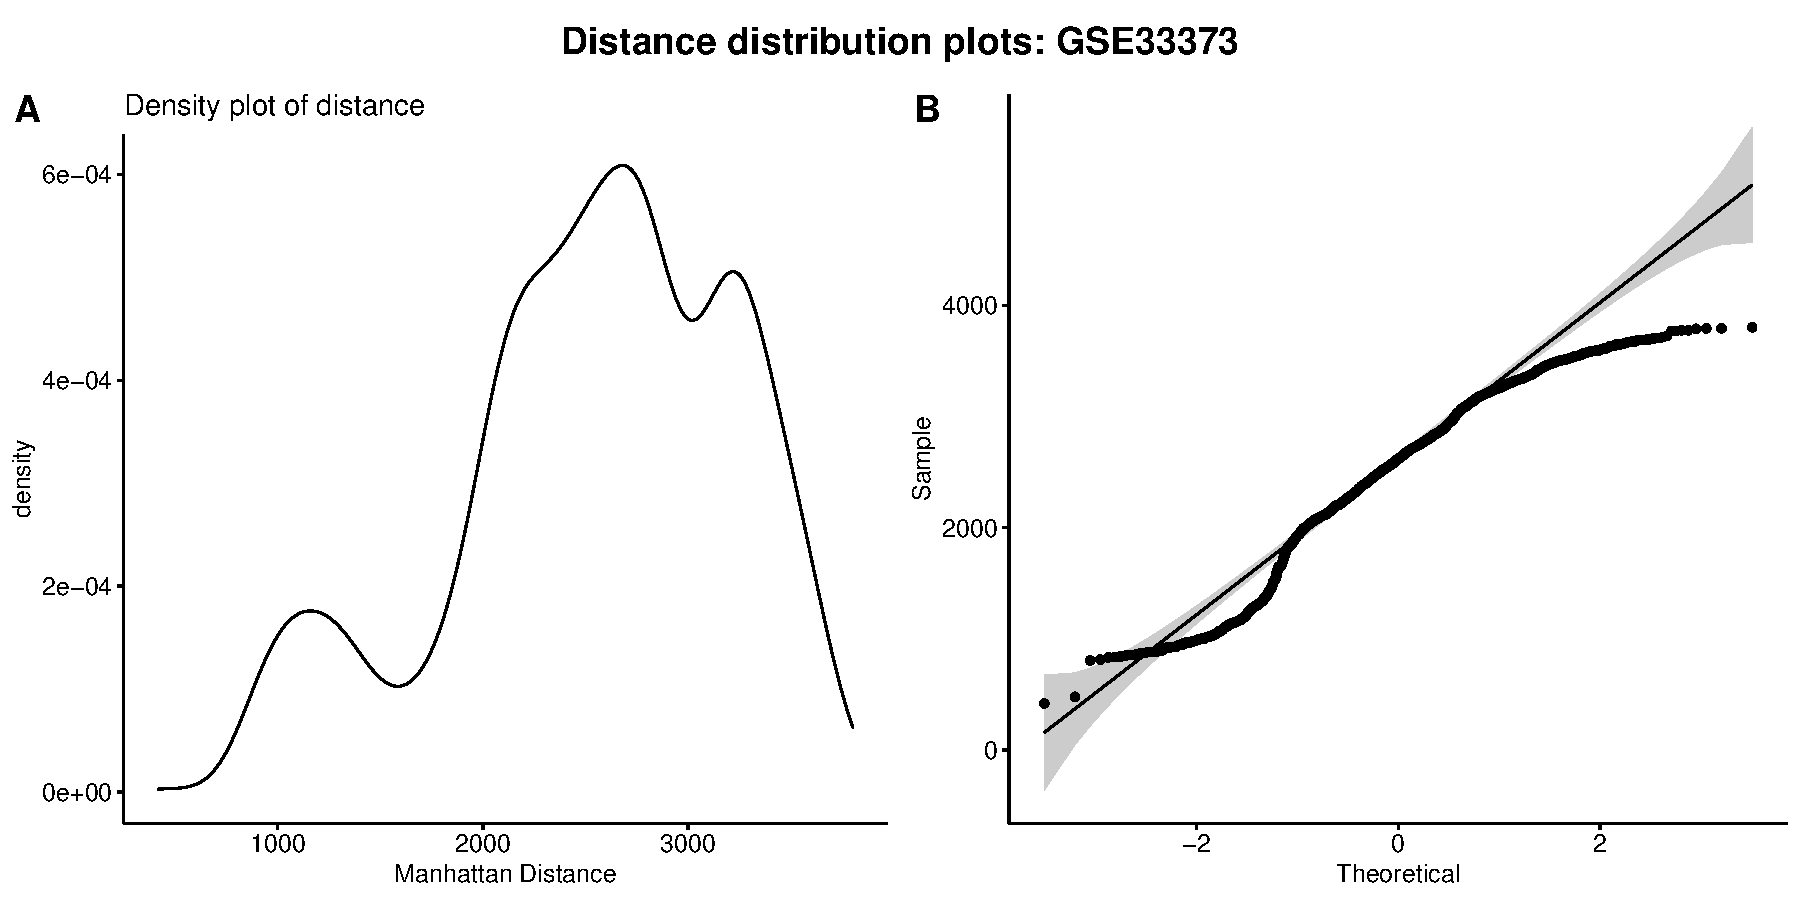
\includegraphics[width=\textwidth]{manhattan-distance_hist_GSE33373.pdf}
	\caption{Density and quantile-quantile plots for distances between samples in GSE33373. \textbf{A} Estimated density curve for distances. \textbf{B} Quantile-quantile plot between theoretical (standard normal) quantiles and sample distance quantiles.}
\end{figure}

\begin{figure}[H]
	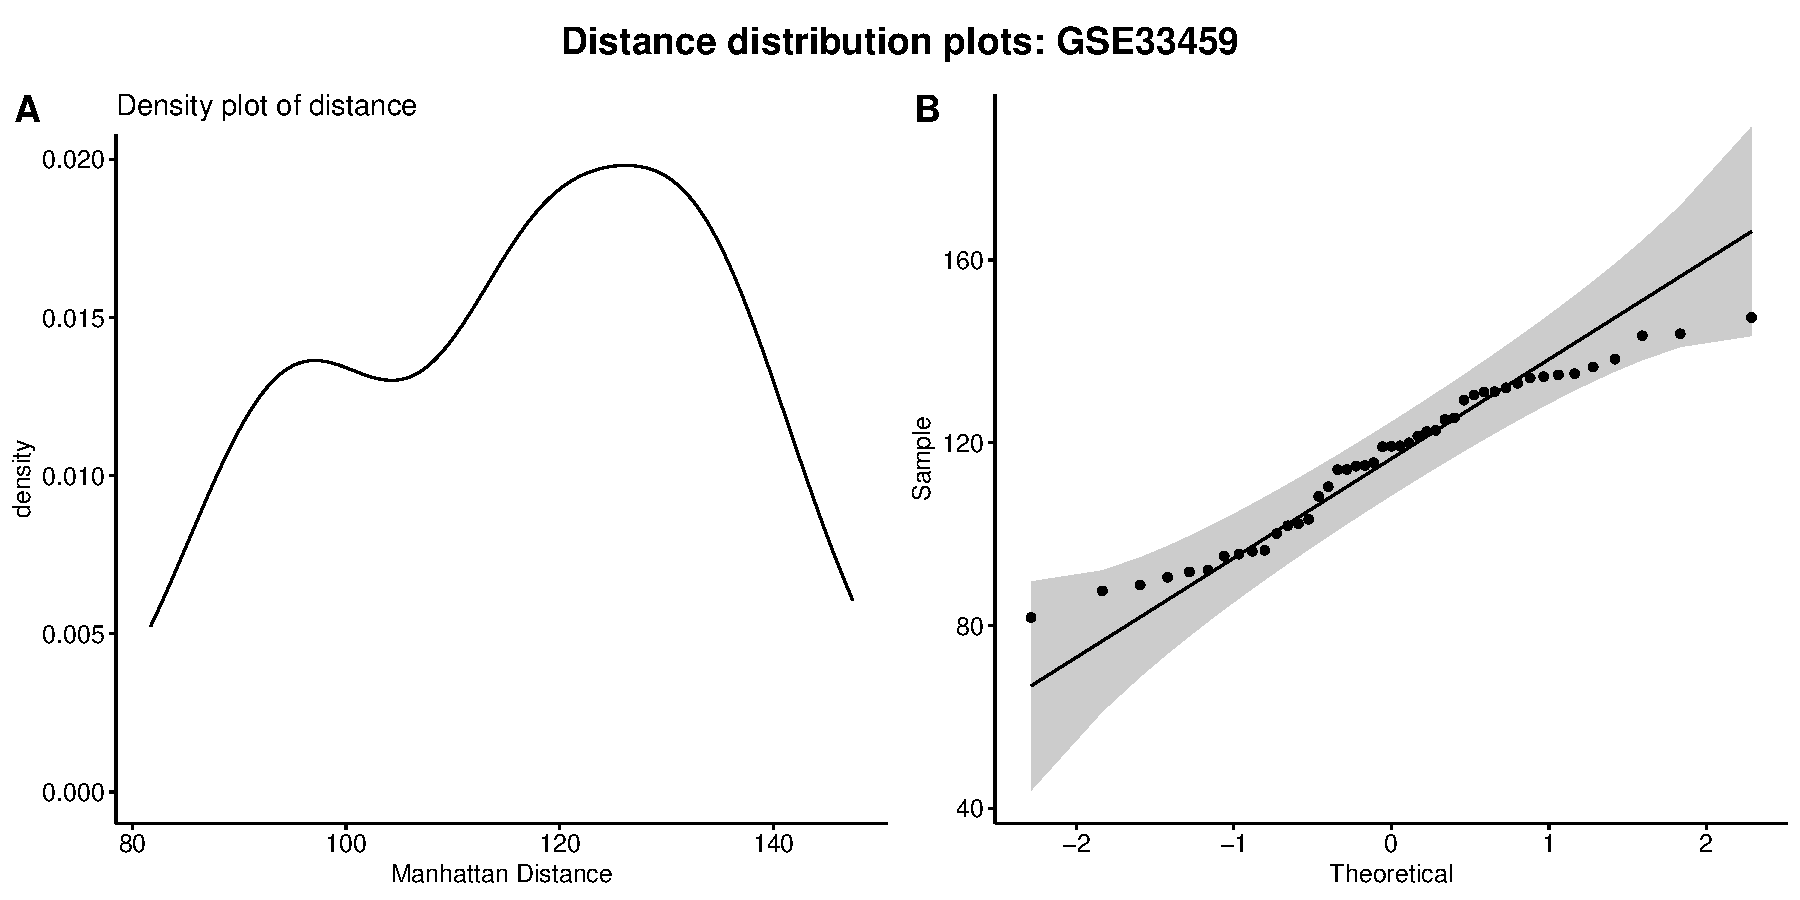
\includegraphics[width=\textwidth]{manhattan-distance_hist_GSE33459.pdf}
	\caption{Density and quantile-quantile plots for distances between samples in GSE33459. \textbf{A} Estimated density curve for distances. \textbf{B} Quantile-quantile plot between theoretical (standard normal) quantiles and sample distance quantiles.}
\end{figure}

\begin{figure}[H]
	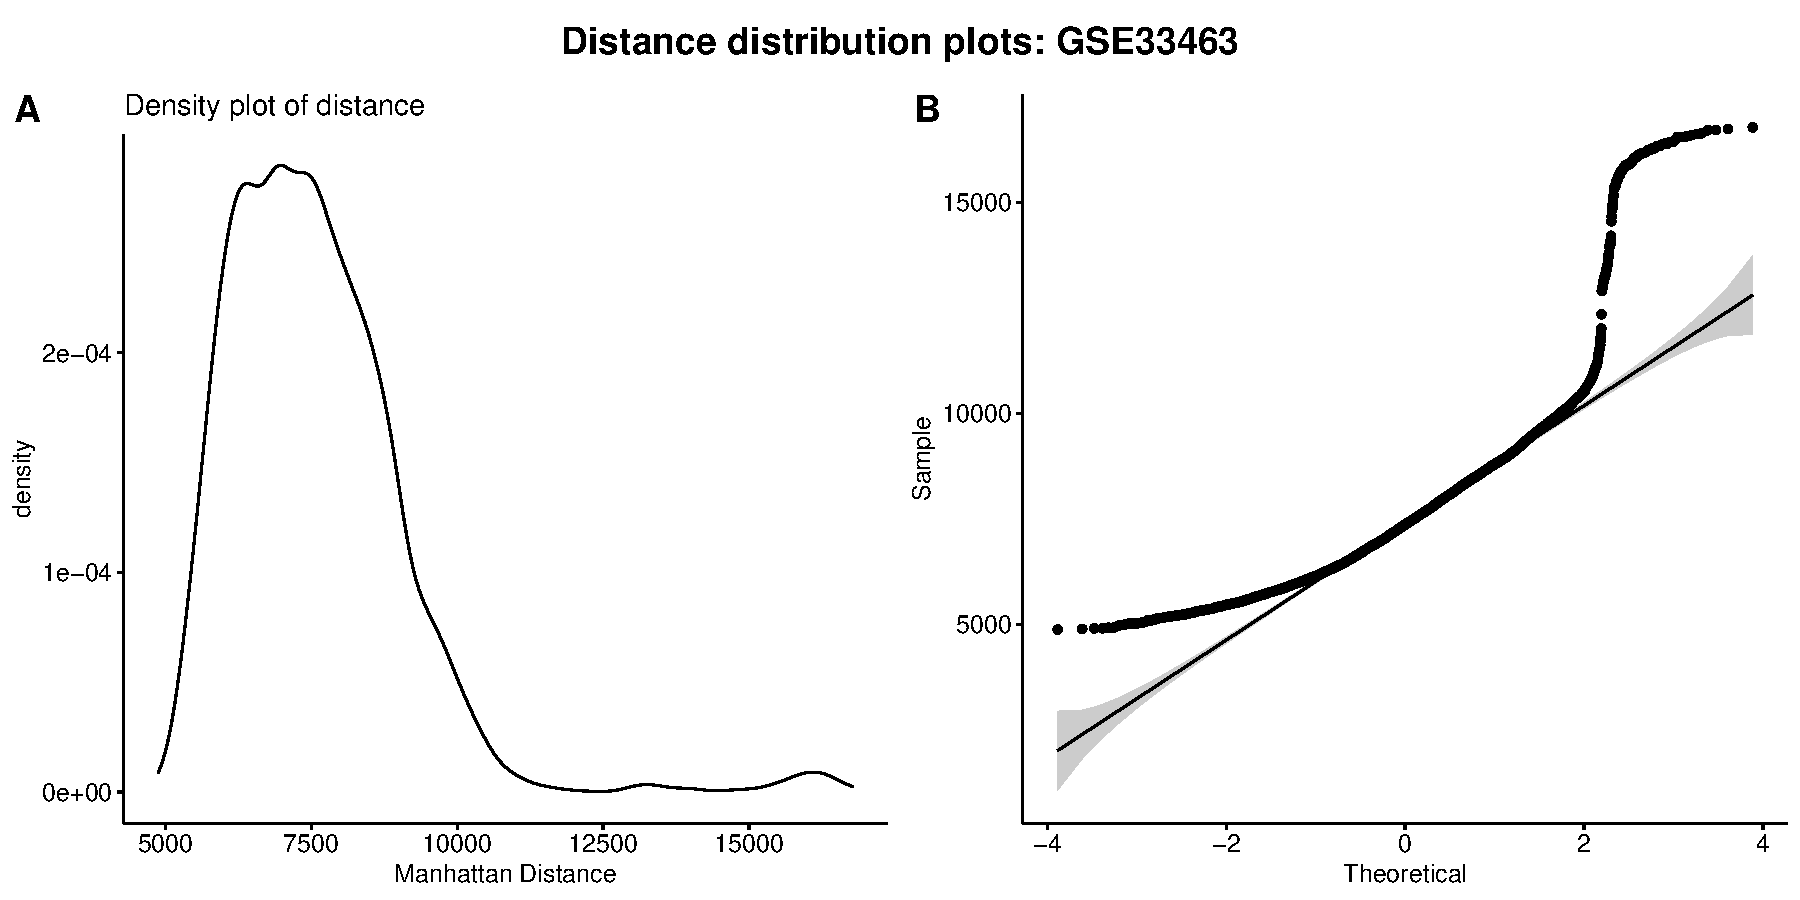
\includegraphics[width=\textwidth]{manhattan-distance_hist_GSE33463.pdf}
	\caption{Density and quantile-quantile plots for distances between samples in GSE33463. \textbf{A} Estimated density curve for distances. \textbf{B} Quantile-quantile plot between theoretical (standard normal) quantiles and sample distance quantiles.}
\end{figure}

\begin{figure}[H]
	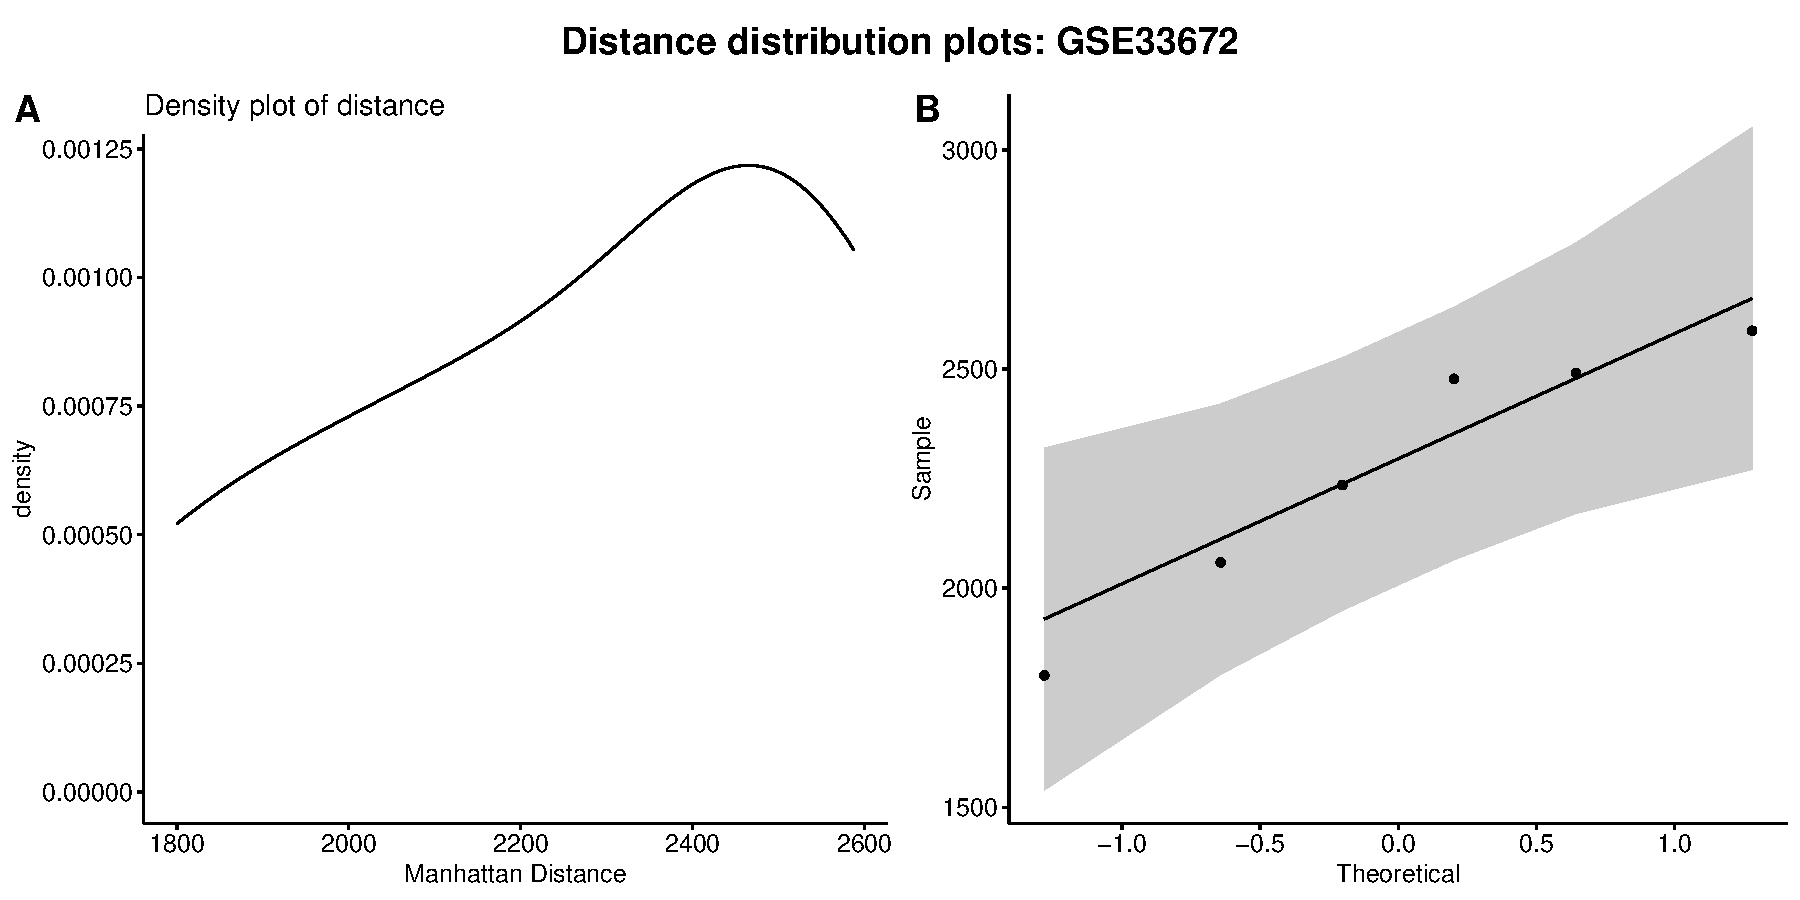
\includegraphics[width=\textwidth]{manhattan-distance_hist_GSE33672.pdf}
	\caption{Density and quantile-quantile plots for distances between samples in GSE33672. \textbf{A} Estimated density curve for distances. \textbf{B} Quantile-quantile plot between theoretical (standard normal) quantiles and sample distance quantiles.}
\end{figure}

\begin{figure}[H]
	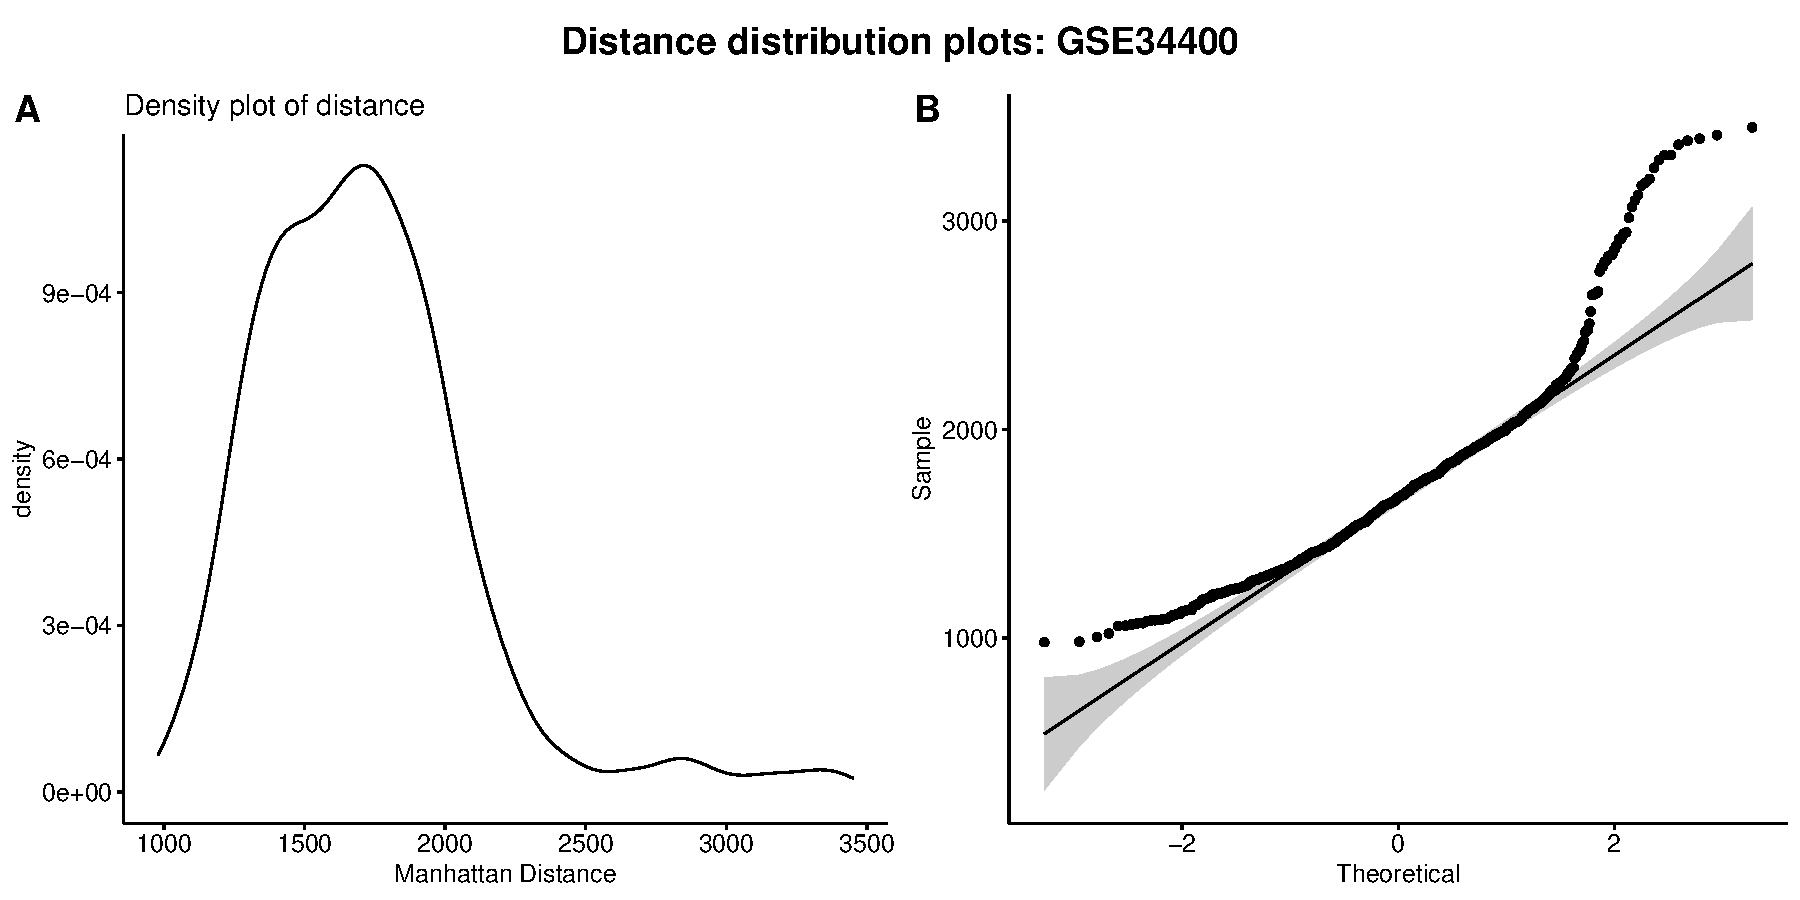
\includegraphics[width=\textwidth]{manhattan-distance_hist_GSE34400.pdf}
	\caption{Density and quantile-quantile plots for distances between samples in GSE34400. \textbf{A} Estimated density curve for distances. \textbf{B} Quantile-quantile plot between theoretical (standard normal) quantiles and sample distance quantiles.}
\end{figure}

\begin{figure}[H]
	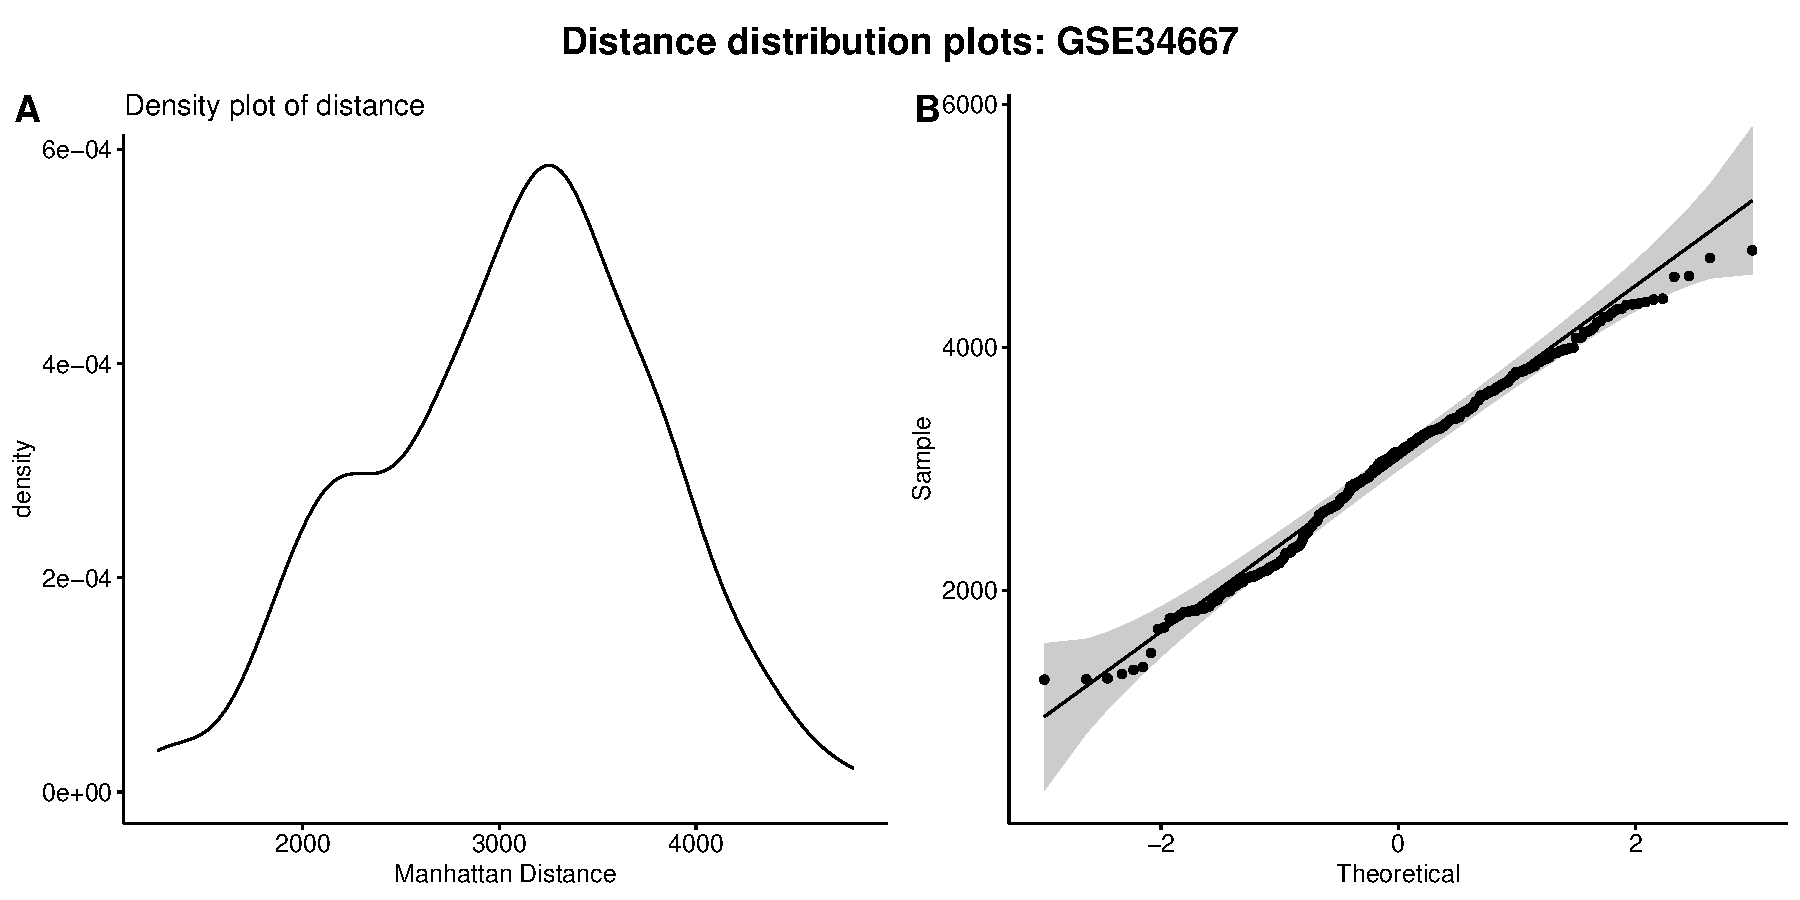
\includegraphics[width=\textwidth]{manhattan-distance_hist_GSE34667.pdf}
	\caption{Density and quantile-quantile plots for distances between samples in GSE34667. \textbf{A} Estimated density curve for distances. \textbf{B} Quantile-quantile plot between theoretical (standard normal) quantiles and sample distance quantiles.}
\end{figure}

\begin{figure}[H]
	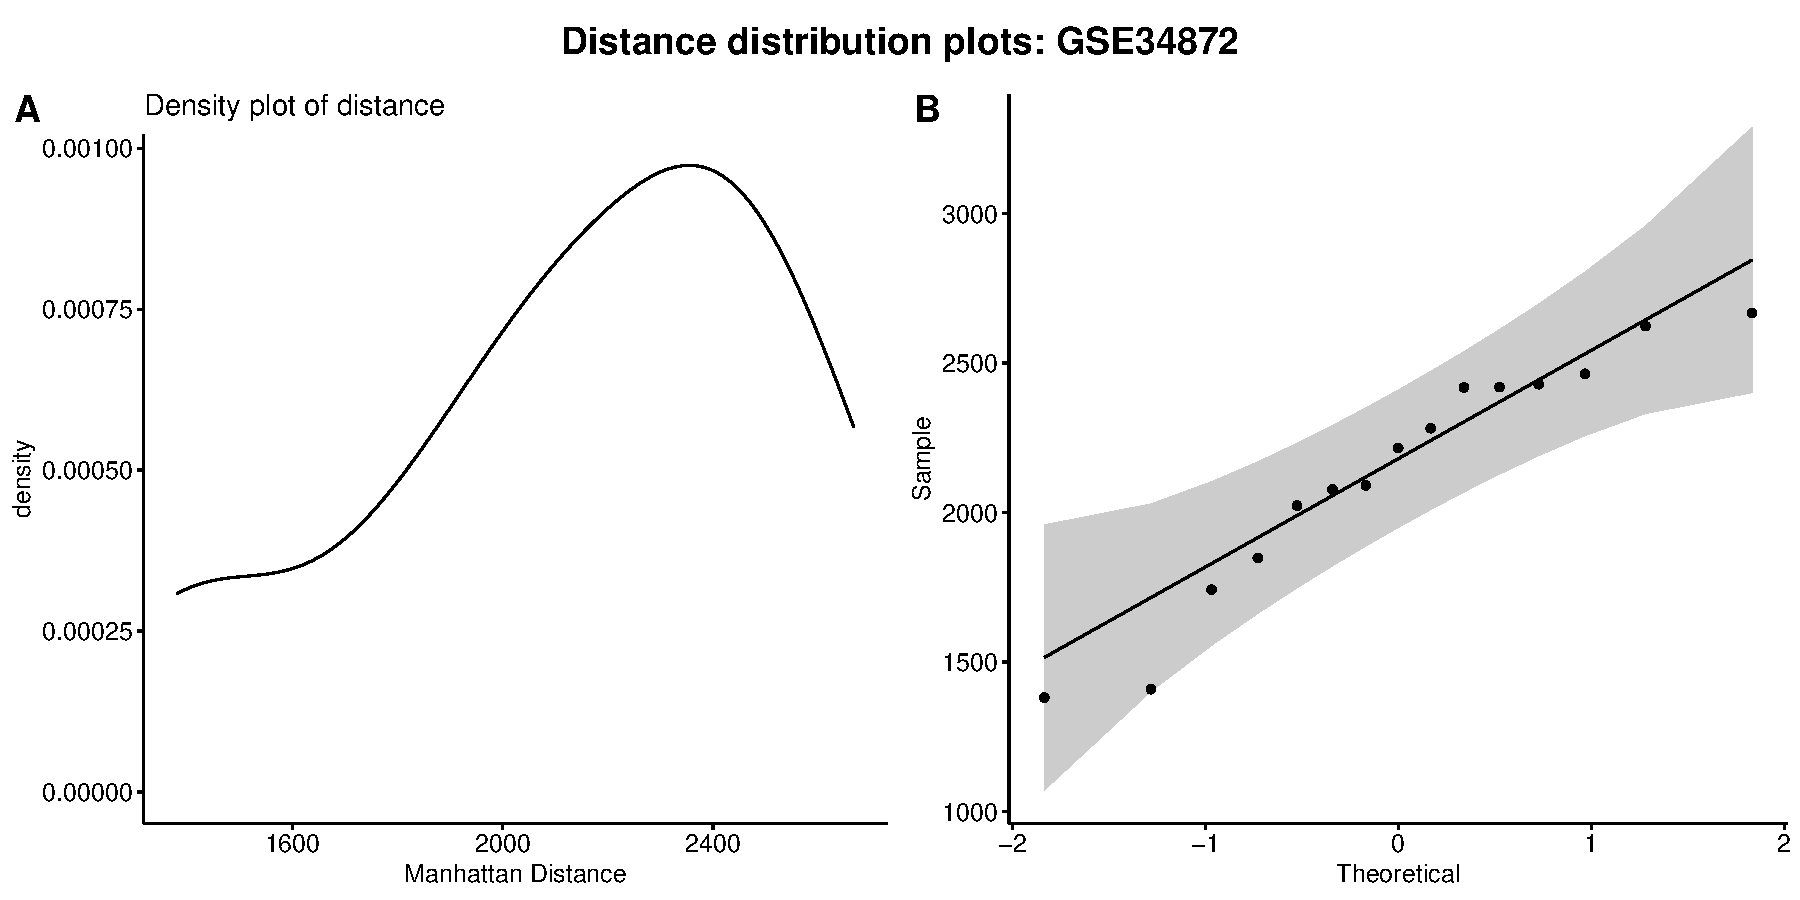
\includegraphics[width=\textwidth]{manhattan-distance_hist_GSE34872.pdf}
	\caption{Density and quantile-quantile plots for distances between samples in GSE34872. \textbf{A} Estimated density curve for distances. \textbf{B} Quantile-quantile plot between theoretical (standard normal) quantiles and sample distance quantiles.}
\end{figure}

\begin{figure}[H]
	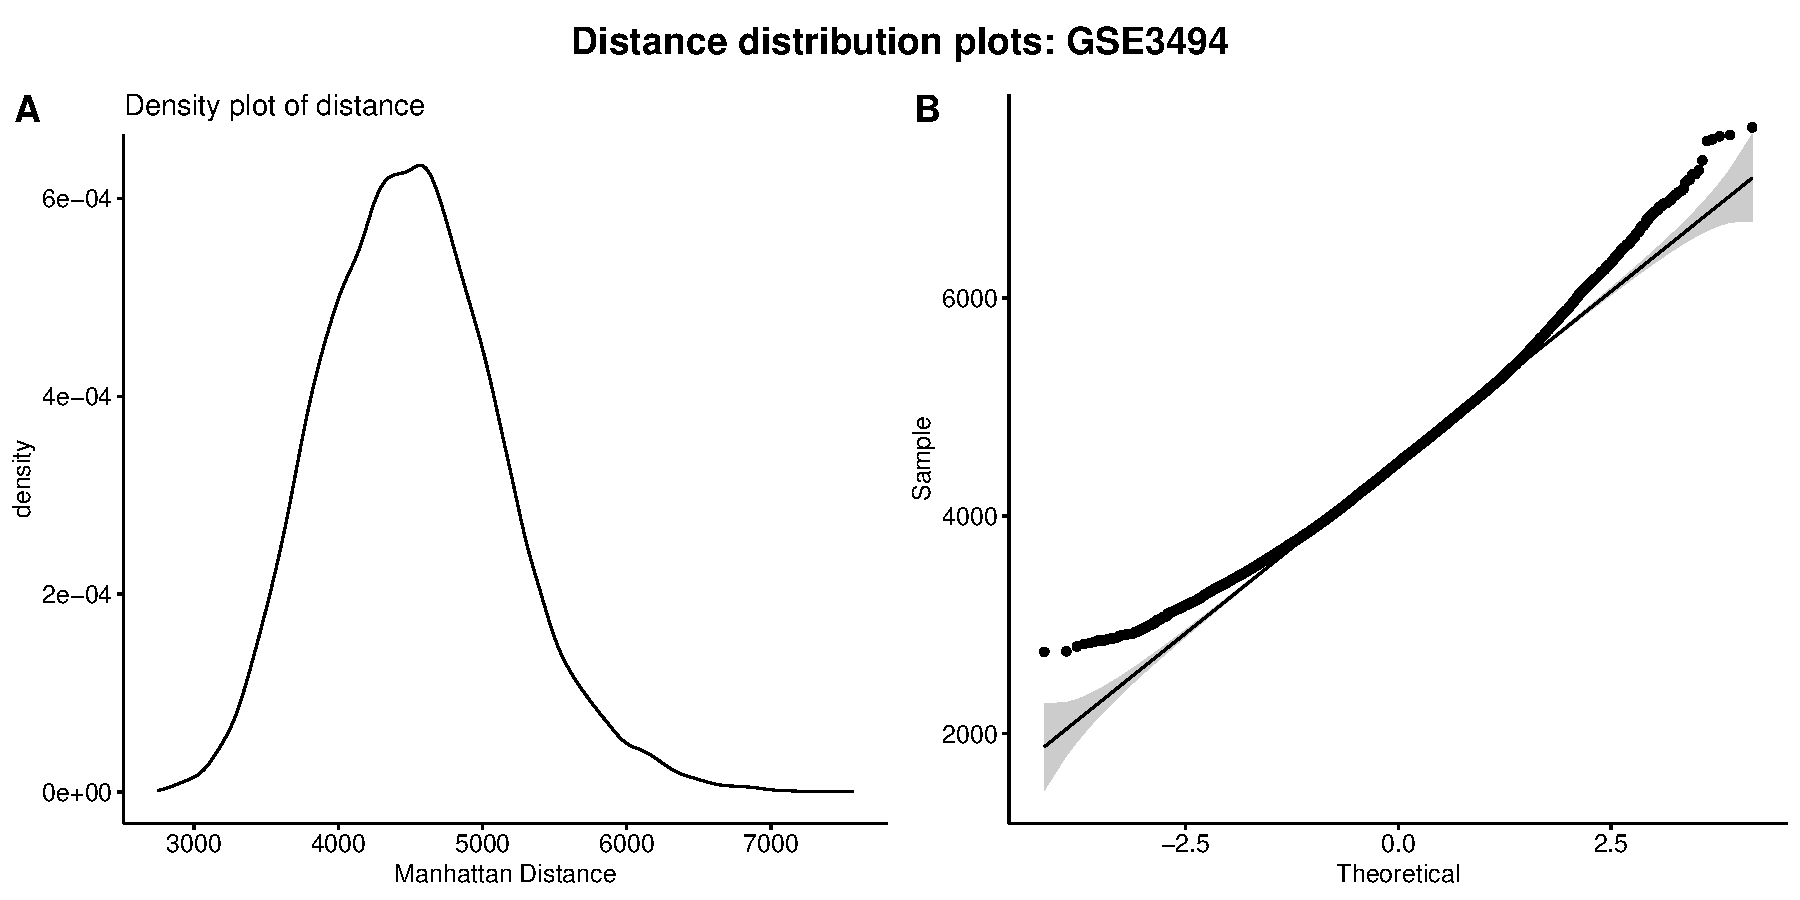
\includegraphics[width=\textwidth]{manhattan-distance_hist_GSE3494.pdf}
	\caption{Density and quantile-quantile plots for distances between samples in GSE3494. \textbf{A} Estimated density curve for distances. \textbf{B} Quantile-quantile plot between theoretical (standard normal) quantiles and sample distance quantiles.}
\end{figure}

\begin{figure}[H]
	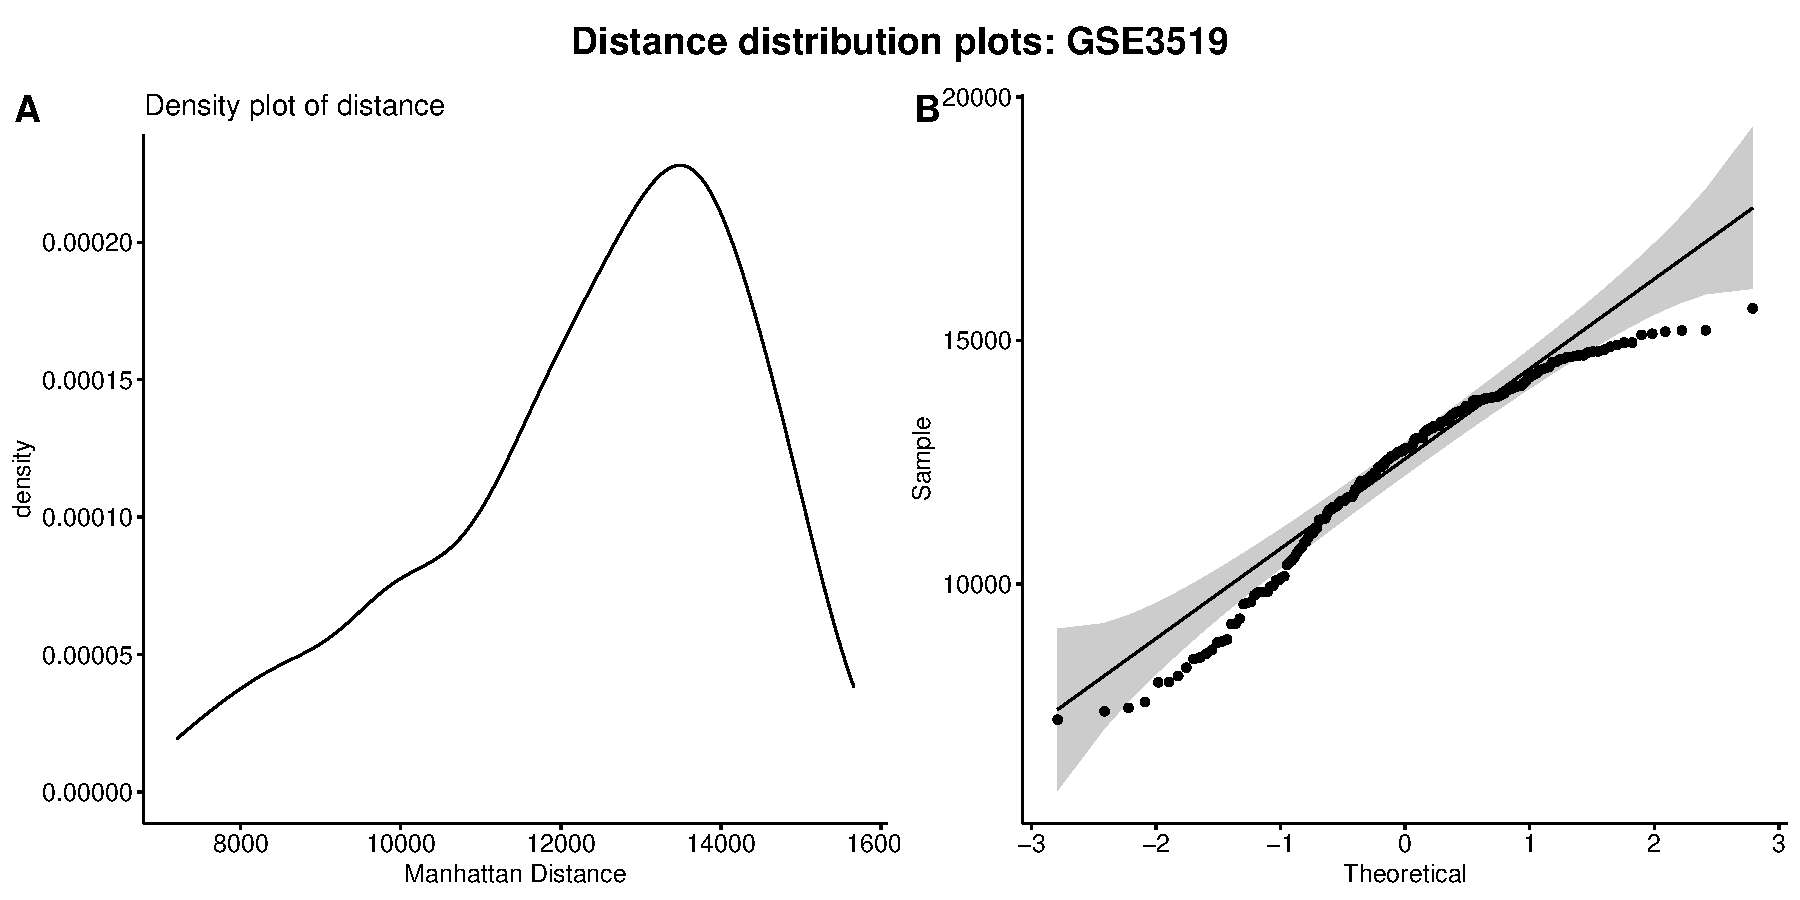
\includegraphics[width=\textwidth]{manhattan-distance_hist_GSE3519.pdf}
	\caption{Density and quantile-quantile plots for distances between samples in GSE3519. \textbf{A} Estimated density curve for distances. \textbf{B} Quantile-quantile plot between theoretical (standard normal) quantiles and sample distance quantiles.}
\end{figure}

\begin{figure}[H]
	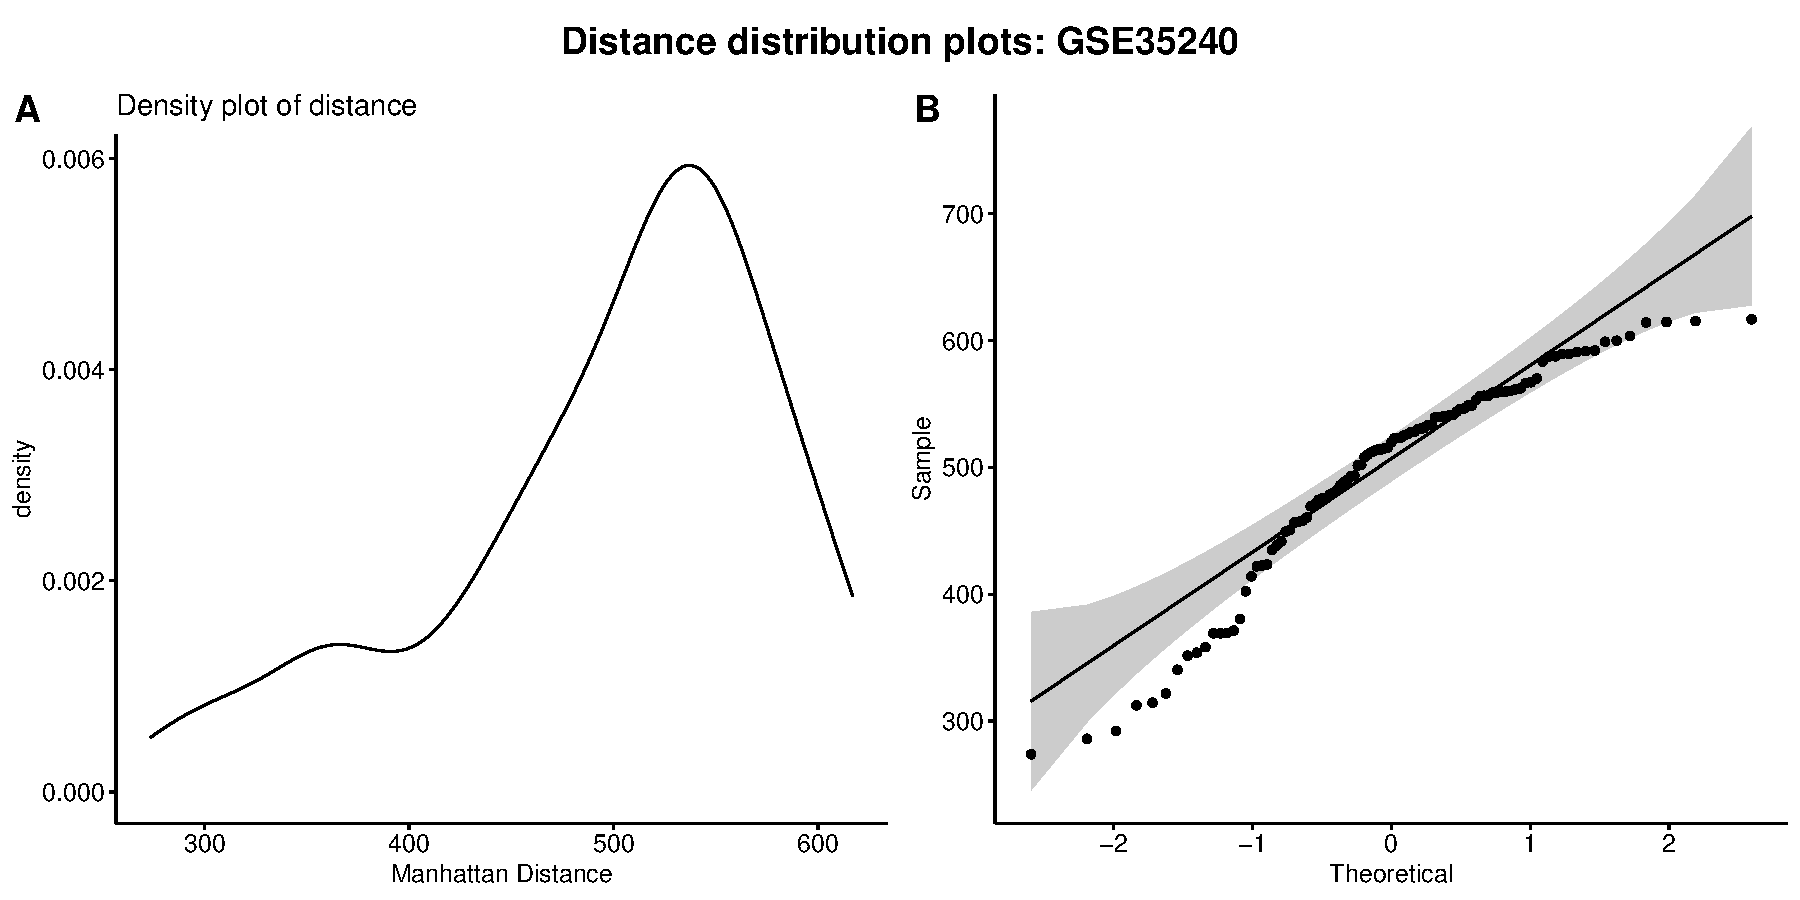
\includegraphics[width=\textwidth]{manhattan-distance_hist_GSE35240.pdf}
	\caption{Density and quantile-quantile plots for distances between samples in GSE35240. \textbf{A} Estimated density curve for distances. \textbf{B} Quantile-quantile plot between theoretical (standard normal) quantiles and sample distance quantiles.}
\end{figure}

\begin{figure}[H]
	\includegraphics[width=\textwidth]{manhattan-distance_hist_GSE37404.pdf}
	\caption{Density and quantile-quantile plots for distances between samples in GSE37404. \textbf{A} Estimated density curve for distances. \textbf{B} Quantile-quantile plot between theoretical (standard normal) quantiles and sample distance quantiles.}
\end{figure}

\begin{figure}[H]
	\includegraphics[width=\textwidth]{manhattan-distance_hist_GSE37902.pdf}
	\caption{Density and quantile-quantile plots for distances between samples in GSE37902. \textbf{A} Estimated density curve for distances. \textbf{B} Quantile-quantile plot between theoretical (standard normal) quantiles and sample distance quantiles.}
\end{figure}

\begin{figure}[H]
	\includegraphics[width=\textwidth]{manhattan-distance_hist_GSE38531.pdf}
	\caption{Density and quantile-quantile plots for distances between samples in GSE38531. \textbf{A} Estimated density curve for distances. \textbf{B} Quantile-quantile plot between theoretical (standard normal) quantiles and sample distance quantiles.}
\end{figure}

\begin{figure}[H]
	\includegraphics[width=\textwidth]{manhattan-distance_hist_GSE38783.pdf}
	\caption{Density and quantile-quantile plots for distances between samples in GSE38783. \textbf{A} Estimated density curve for distances. \textbf{B} Quantile-quantile plot between theoretical (standard normal) quantiles and sample distance quantiles.}
\end{figure}

\begin{figure}[H]
	\includegraphics[width=\textwidth]{manhattan-distance_hist_GSE39549.pdf}
	\caption{Density and quantile-quantile plots for distances between samples in GSE39549. \textbf{A} Estimated density curve for distances. \textbf{B} Quantile-quantile plot between theoretical (standard normal) quantiles and sample distance quantiles.}
\end{figure}

\begin{figure}[H]
	\includegraphics[width=\textwidth]{manhattan-distance_hist_GSE41221.pdf}
	\caption{Density and quantile-quantile plots for distances between samples in GSE41221. \textbf{A} Estimated density curve for distances. \textbf{B} Quantile-quantile plot between theoretical (standard normal) quantiles and sample distance quantiles.}
\end{figure}

\begin{figure}[H]
	\includegraphics[width=\textwidth]{manhattan-distance_hist_GSE46727.pdf}
	\caption{Density and quantile-quantile plots for distances between samples in GSE46727. \textbf{A} Estimated density curve for distances. \textbf{B} Quantile-quantile plot between theoretical (standard normal) quantiles and sample distance quantiles.}
\end{figure}

\begin{figure}[H]
	\includegraphics[width=\textwidth]{manhattan-distance_hist_GSE46728.pdf}
	\caption{Density and quantile-quantile plots for distances between samples in GSE46728. \textbf{A} Estimated density curve for distances. \textbf{B} Quantile-quantile plot between theoretical (standard normal) quantiles and sample distance quantiles.}
\end{figure}

\begin{figure}[H]
	\includegraphics[width=\textwidth]{manhattan-distance_hist_GSE47406.pdf}
	\caption{Density and quantile-quantile plots for distances between samples in GSE47406. \textbf{A} Estimated density curve for distances. \textbf{B} Quantile-quantile plot between theoretical (standard normal) quantiles and sample distance quantiles.}
\end{figure}

\begin{figure}[H]
	\includegraphics[width=\textwidth]{manhattan-distance_hist_GSE48964.pdf}
	\caption{Density and quantile-quantile plots for distances between samples in GSE48964. \textbf{A} Estimated density curve for distances. \textbf{B} Quantile-quantile plot between theoretical (standard normal) quantiles and sample distance quantiles.}
\end{figure}

\begin{figure}[H]
	\includegraphics[width=\textwidth]{manhattan-distance_hist_GSE49382.pdf}
	\caption{Density and quantile-quantile plots for distances between samples in GSE49382. \textbf{A} Estimated density curve for distances. \textbf{B} Quantile-quantile plot between theoretical (standard normal) quantiles and sample distance quantiles.}
\end{figure}

\begin{figure}[H]
	\includegraphics[width=\textwidth]{manhattan-distance_hist_GSE49486.pdf}
	\caption{Density and quantile-quantile plots for distances between samples in GSE49486. \textbf{A} Estimated density curve for distances. \textbf{B} Quantile-quantile plot between theoretical (standard normal) quantiles and sample distance quantiles.}
\end{figure}

\begin{figure}[H]
	\includegraphics[width=\textwidth]{manhattan-distance_hist_GSE50604.pdf}
	\caption{Density and quantile-quantile plots for distances between samples in GSE50604. \textbf{A} Estimated density curve for distances. \textbf{B} Quantile-quantile plot between theoretical (standard normal) quantiles and sample distance quantiles.}
\end{figure}

\begin{figure}[H]
	\includegraphics[width=\textwidth]{manhattan-distance_hist_GSE5281.pdf}
	\caption{Density and quantile-quantile plots for distances between samples in GSE5281. \textbf{A} Estimated density curve for distances. \textbf{B} Quantile-quantile plot between theoretical (standard normal) quantiles and sample distance quantiles.}
\end{figure}

\begin{figure}[H]
	\includegraphics[width=\textwidth]{manhattan-distance_hist_GSE53122.pdf}
	\caption{Density and quantile-quantile plots for distances between samples in GSE53122. \textbf{A} Estimated density curve for distances. \textbf{B} Quantile-quantile plot between theoretical (standard normal) quantiles and sample distance quantiles.}
\end{figure}

\begin{figure}[H]
	\includegraphics[width=\textwidth]{manhattan-distance_hist_GSE54129.pdf}
	\caption{Density and quantile-quantile plots for distances between samples in GSE54129. \textbf{A} Estimated density curve for distances. \textbf{B} Quantile-quantile plot between theoretical (standard normal) quantiles and sample distance quantiles.}
\end{figure}

\begin{figure}[H]
	\includegraphics[width=\textwidth]{manhattan-distance_hist_GSE54216.pdf}
	\caption{Density and quantile-quantile plots for distances between samples in GSE54216. \textbf{A} Estimated density curve for distances. \textbf{B} Quantile-quantile plot between theoretical (standard normal) quantiles and sample distance quantiles.}
\end{figure}

\begin{figure}[H]
	\includegraphics[width=\textwidth]{manhattan-distance_hist_GSE54350.pdf}
	\caption{Density and quantile-quantile plots for distances between samples in GSE54350. \textbf{A} Estimated density curve for distances. \textbf{B} Quantile-quantile plot between theoretical (standard normal) quantiles and sample distance quantiles.}
\end{figure}

\begin{figure}[H]
	\includegraphics[width=\textwidth]{manhattan-distance_hist_GSE54917.pdf}
	\caption{Density and quantile-quantile plots for distances between samples in GSE54917. \textbf{A} Estimated density curve for distances. \textbf{B} Quantile-quantile plot between theoretical (standard normal) quantiles and sample distance quantiles.}
\end{figure}

\begin{figure}[H]
	\includegraphics[width=\textwidth]{manhattan-distance_hist_GSE55503.pdf}
	\caption{Density and quantile-quantile plots for distances between samples in GSE55503. \textbf{A} Estimated density curve for distances. \textbf{B} Quantile-quantile plot between theoretical (standard normal) quantiles and sample distance quantiles.}
\end{figure}

\begin{figure}[H]
	\includegraphics[width=\textwidth]{manhattan-distance_hist_GSE57002.pdf}
	\caption{Density and quantile-quantile plots for distances between samples in GSE57002. \textbf{A} Estimated density curve for distances. \textbf{B} Quantile-quantile plot between theoretical (standard normal) quantiles and sample distance quantiles.}
\end{figure}

\begin{figure}[H]
	\includegraphics[width=\textwidth]{manhattan-distance_hist_GSE5859.pdf}
	\caption{Density and quantile-quantile plots for distances between samples in GSE5859. \textbf{A} Estimated density curve for distances. \textbf{B} Quantile-quantile plot between theoretical (standard normal) quantiles and sample distance quantiles.}
\end{figure}

\begin{figure}[H]
	\includegraphics[width=\textwidth]{manhattan-distance_hist_GSE61140.pdf}
	\caption{Density and quantile-quantile plots for distances between samples in GSE61140. \textbf{A} Estimated density curve for distances. \textbf{B} Quantile-quantile plot between theoretical (standard normal) quantiles and sample distance quantiles.}
\end{figure}

\begin{figure}[H]
	\includegraphics[width=\textwidth]{manhattan-distance_hist_GSE62598.pdf}
	\caption{Density and quantile-quantile plots for distances between samples in GSE62598. \textbf{A} Estimated density curve for distances. \textbf{B} Quantile-quantile plot between theoretical (standard normal) quantiles and sample distance quantiles.}
\end{figure}

\begin{figure}[H]
	\includegraphics[width=\textwidth]{manhattan-distance_hist_GSE6414.pdf}
	\caption{Density and quantile-quantile plots for distances between samples in GSE6414. \textbf{A} Estimated density curve for distances. \textbf{B} Quantile-quantile plot between theoretical (standard normal) quantiles and sample distance quantiles.}
\end{figure}

\begin{figure}[H]
	\includegraphics[width=\textwidth]{manhattan-distance_hist_GSE64670.pdf}
	\caption{Density and quantile-quantile plots for distances between samples in GSE64670. \textbf{A} Estimated density curve for distances. \textbf{B} Quantile-quantile plot between theoretical (standard normal) quantiles and sample distance quantiles.}
\end{figure}

\begin{figure}[H]
	\includegraphics[width=\textwidth]{manhattan-distance_hist_GSE64718.pdf}
	\caption{Density and quantile-quantile plots for distances between samples in GSE64718. \textbf{A} Estimated density curve for distances. \textbf{B} Quantile-quantile plot between theoretical (standard normal) quantiles and sample distance quantiles.}
\end{figure}

\begin{figure}[H]
	\includegraphics[width=\textwidth]{manhattan-distance_hist_GSE65517.pdf}
	\caption{Density and quantile-quantile plots for distances between samples in GSE65517. \textbf{A} Estimated density curve for distances. \textbf{B} Quantile-quantile plot between theoretical (standard normal) quantiles and sample distance quantiles.}
\end{figure}

\begin{figure}[H]
	\includegraphics[width=\textwidth]{manhattan-distance_hist_GSE6720.pdf}
	\caption{Density and quantile-quantile plots for distances between samples in GSE6720. \textbf{A} Estimated density curve for distances. \textbf{B} Quantile-quantile plot between theoretical (standard normal) quantiles and sample distance quantiles.}
\end{figure}

\begin{figure}[H]
	\includegraphics[width=\textwidth]{manhattan-distance_hist_GSE67376.pdf}
	\caption{Density and quantile-quantile plots for distances between samples in GSE67376. \textbf{A} Estimated density curve for distances. \textbf{B} Quantile-quantile plot between theoretical (standard normal) quantiles and sample distance quantiles.}
\end{figure}

\begin{figure}[H]
	\includegraphics[width=\textwidth]{manhattan-distance_hist_GSE67492.pdf}
	\caption{Density and quantile-quantile plots for distances between samples in GSE67492. \textbf{A} Estimated density curve for distances. \textbf{B} Quantile-quantile plot between theoretical (standard normal) quantiles and sample distance quantiles.}
\end{figure}

\begin{figure}[H]
	\includegraphics[width=\textwidth]{manhattan-distance_hist_GSE67865.pdf}
	\caption{Density and quantile-quantile plots for distances between samples in GSE67865. \textbf{A} Estimated density curve for distances. \textbf{B} Quantile-quantile plot between theoretical (standard normal) quantiles and sample distance quantiles.}
\end{figure}

\begin{figure}[H]
	\includegraphics[width=\textwidth]{manhattan-distance_hist_GSE68918.pdf}
	\caption{Density and quantile-quantile plots for distances between samples in GSE68918. \textbf{A} Estimated density curve for distances. \textbf{B} Quantile-quantile plot between theoretical (standard normal) quantiles and sample distance quantiles.}
\end{figure}

\begin{figure}[H]
	\includegraphics[width=\textwidth]{manhattan-distance_hist_GSE7124.pdf}
	\caption{Density and quantile-quantile plots for distances between samples in GSE7124. \textbf{A} Estimated density curve for distances. \textbf{B} Quantile-quantile plot between theoretical (standard normal) quantiles and sample distance quantiles.}
\end{figure}

\begin{figure}[H]
	\includegraphics[width=\textwidth]{manhattan-distance_hist_GSE71868.pdf}
	\caption{Density and quantile-quantile plots for distances between samples in GSE71868. \textbf{A} Estimated density curve for distances. \textbf{B} Quantile-quantile plot between theoretical (standard normal) quantiles and sample distance quantiles.}
\end{figure}

\begin{figure}[H]
	\includegraphics[width=\textwidth]{manhattan-distance_hist_GSE7197.pdf}
	\caption{Density and quantile-quantile plots for distances between samples in GSE7197. \textbf{A} Estimated density curve for distances. \textbf{B} Quantile-quantile plot between theoretical (standard normal) quantiles and sample distance quantiles.}
\end{figure}

\begin{figure}[H]
	\includegraphics[width=\textwidth]{manhattan-distance_hist_GSE75037.pdf}
	\caption{Density and quantile-quantile plots for distances between samples in GSE75037. \textbf{A} Estimated density curve for distances. \textbf{B} Quantile-quantile plot between theoretical (standard normal) quantiles and sample distance quantiles.}
\end{figure}

\begin{figure}[H]
	\includegraphics[width=\textwidth]{manhattan-distance_hist_GSE7511.pdf}
	\caption{Density and quantile-quantile plots for distances between samples in GSE7511. \textbf{A} Estimated density curve for distances. \textbf{B} Quantile-quantile plot between theoretical (standard normal) quantiles and sample distance quantiles.}
\end{figure}

\begin{figure}[H]
	\includegraphics[width=\textwidth]{manhattan-distance_hist_GSE7567.pdf}
	\caption{Density and quantile-quantile plots for distances between samples in GSE7567. \textbf{A} Estimated density curve for distances. \textbf{B} Quantile-quantile plot between theoretical (standard normal) quantiles and sample distance quantiles.}
\end{figure}

\begin{figure}[H]
	\includegraphics[width=\textwidth]{manhattan-distance_hist_GSE7592.pdf}
	\caption{Density and quantile-quantile plots for distances between samples in GSE7592. \textbf{A} Estimated density curve for distances. \textbf{B} Quantile-quantile plot between theoretical (standard normal) quantiles and sample distance quantiles.}
\end{figure}

\begin{figure}[H]
	\includegraphics[width=\textwidth]{manhattan-distance_hist_GSE7670.pdf}
	\caption{Density and quantile-quantile plots for distances between samples in GSE7670. \textbf{A} Estimated density curve for distances. \textbf{B} Quantile-quantile plot between theoretical (standard normal) quantiles and sample distance quantiles.}
\end{figure}

\begin{figure}[H]
	\includegraphics[width=\textwidth]{manhattan-distance_hist_GSE7881.pdf}
	\caption{Density and quantile-quantile plots for distances between samples in GSE7881. \textbf{A} Estimated density curve for distances. \textbf{B} Quantile-quantile plot between theoretical (standard normal) quantiles and sample distance quantiles.}
\end{figure}

\begin{figure}[H]
	\includegraphics[width=\textwidth]{manhattan-distance_hist_GSE79973.pdf}
	\caption{Density and quantile-quantile plots for distances between samples in GSE79973. \textbf{A} Estimated density curve for distances. \textbf{B} Quantile-quantile plot between theoretical (standard normal) quantiles and sample distance quantiles.}
\end{figure}

\begin{figure}[H]
	\includegraphics[width=\textwidth]{manhattan-distance_hist_GSE83077.pdf}
	\caption{Density and quantile-quantile plots for distances between samples in GSE83077. \textbf{A} Estimated density curve for distances. \textbf{B} Quantile-quantile plot between theoretical (standard normal) quantiles and sample distance quantiles.}
\end{figure}

\begin{figure}[H]
	\includegraphics[width=\textwidth]{manhattan-distance_hist_GSE8498.pdf}
	\caption{Density and quantile-quantile plots for distances between samples in GSE8498. \textbf{A} Estimated density curve for distances. \textbf{B} Quantile-quantile plot between theoretical (standard normal) quantiles and sample distance quantiles.}
\end{figure}

\begin{figure}[H]
	\includegraphics[width=\textwidth]{manhattan-distance_hist_GSE9687.pdf}
	\caption{Density and quantile-quantile plots for distances between samples in GSE9687. \textbf{A} Estimated density curve for distances. \textbf{B} Quantile-quantile plot between theoretical (standard normal) quantiles and sample distance quantiles.}
\end{figure}

\begin{figure}[H]
	\includegraphics[width=\textwidth]{manhattan-distance_hist_GSE9820.pdf}
	\caption{Density and quantile-quantile plots for distances between samples in GSE9820. \textbf{A} Estimated density curve for distances. \textbf{B} Quantile-quantile plot between theoretical (standard normal) quantiles and sample distance quantiles.}
\end{figure}

\begin{figure}[H]
	\includegraphics[width=\textwidth]{manhattan-distance_hist_GSE98634.pdf}
	\caption{Density and quantile-quantile plots for distances between samples in GSE98634. \textbf{A} Estimated density curve for distances. \textbf{B} Quantile-quantile plot between theoretical (standard normal) quantiles and sample distance quantiles.}
\end{figure}

\begin{figure}[H]
	\includegraphics[width=\textwidth]{manhattan-distance_hist_GSE99295.pdf}
	\caption{Density and quantile-quantile plots for distances between samples in GSE99295. \textbf{A} Estimated density curve for distances. \textbf{B} Quantile-quantile plot between theoretical (standard normal) quantiles and sample distance quantiles.}
\end{figure}

\begin{figure}[H]
	\includegraphics[width=\textwidth]{manhattan-distance_hist_GSE48200.pdf}
	\caption{Density and quantile-quantile plots for distances between samples in GSE48200. \textbf{A} Estimated density curve for distances. \textbf{B} Quantile-quantile plot between theoretical (standard normal) quantiles and sample distance quantiles.}
\end{figure}

%\bibliographystyle{unsrt}
%\bibliography{BoD}   % name of bib file
\end{document}
